%definira klasu dokumenta 
\documentclass[12pt]{report} 

%prostor izmedu naredbi \documentclass i \begin{document} se zove uvod. U njemu se nalaze naredbe koje se odnose na cijeli dokument

%osnovni LaTex ne može riješiti sve probleme, pa se koriste različiti paketi koji olakšavaju izradu željenog dokumenta
\usepackage[croatian]{babel} 
\usepackage{amssymb}
\usepackage{amsmath}
\usepackage{txfonts}
\usepackage{mathdots}
\usepackage{titlesec}
\usepackage{array}
\usepackage{lastpage}
\usepackage{etoolbox}
\usepackage{tabularray}
\usepackage{color, colortbl}
\usepackage{adjustbox}
\usepackage{geometry}
\usepackage[classicReIm]{kpfonts}
\usepackage{hyperref}
\usepackage{fancyhdr}

\usepackage{float}
\usepackage{setspace}
\restylefloat{table}


\patchcmd{\chapter}{\thispagestyle{plain}}{\thispagestyle{fancy}}{}{} %redefiniranje stila stranice u paketu fancyhdr

%oblik naslova poglavlja
\titleformat{\chapter}{\normalfont\huge\bfseries}{\thechapter.}{20pt}{\Huge}
\titlespacing{\chapter}{0pt}{0pt}{40pt}


\linespread{1.3} %razmak između redaka

\geometry{a4paper, left=1in, top=1in,}  %oblik stranice

\hypersetup{ colorlinks, citecolor=black, filecolor=black, linkcolor=black,	urlcolor=black }   %izgled poveznice


%prored smanjen između redaka u nabrajanjima i popisima
\newenvironment{packed_enum}{
	\begin{enumerate}
		\setlength{\itemsep}{0pt}
		\setlength{\parskip}{0pt}
		\setlength{\parsep}{0pt}
	}{\end{enumerate}}

\newenvironment{packed_item}{
	\begin{itemize}
		\setlength{\itemsep}{0pt}
		\setlength{\parskip}{0pt}
		\setlength{\parsep}{0pt}
	}{\end{itemize}}




%boja za privatni i udaljeni kljuc u tablicama
\definecolor{LightBlue}{rgb}{0.9,0.9,1}
\definecolor{LightGreen}{rgb}{0.9,1,0.9}

%Promjena teksta za dugačke tablice
\DefTblrTemplate{contfoot-text}{normal}{Nastavljeno na idućoj stranici}
\SetTblrTemplate{contfoot-text}{normal}
\DefTblrTemplate{conthead-text}{normal}{(Nastavljeno)}
\SetTblrTemplate{conthead-text}{normal}
\DefTblrTemplate{middlehead,lasthead}{normal}{Nastavljeno od prethodne stranice}
\SetTblrTemplate{middlehead,lasthead}{normal}

%podesavanje zaglavlja i podnožja

\pagestyle{fancy}
\lhead{Programsko inženjerstvo}
\rhead{KuhajIT}
\lfoot{30Bodova}
\cfoot{stranica \thepage/\pageref{LastPage}}
\rfoot{\today}
\renewcommand{\headrulewidth}{0.2pt}
\renewcommand{\footrulewidth}{0.2pt}


\begin{document} 
	
	
	
	\begin{titlepage}
		\begin{center}
			\vspace*{\stretch{1.0}} %u kombinaciji s ostalim \vspace naredbama definira razmak između redaka teksta
			\LARGE Programsko inženjerstvo\\
			\large Ak. god. 2023./2024.\\
			
			\vspace*{\stretch{3.0}}
			
			\huge KuhajIT\\
			\Large Dokumentacija, Rev. \textit{1}\\
			
			\vspace*{\stretch{12.0}}
			\normalsize
			Grupa: \textit{30Bodova}\\
			Voditelj: \textit{Hana Ivančić}\\
			
			
			\vspace*{\stretch{1.0}}
			Datum predaje: \textit{17. 11. 2023.}\\
	
			\vspace*{\stretch{4.0}}
			
			Nastavnik: \textit{mag. ing. Hrvoje Nuić}\\
		
		\end{center}

	
	\end{titlepage}

	
	\tableofcontents


	\chapter{Dnevnik promjena dokumentacije}
		
		\begin{longtblr}[
				label=none
			]{
				width = \textwidth, 
				colspec={|X[2]|X[10]|X[4]|X[3]|}, 
				rowhead = 1
			}
			\hline
			\textbf{Rev.}	& \textbf{Opis promjene/dodatka} & \textbf{Autori} & \textbf{Datum}\\[3pt] \hline
			0.1 & Napravljen predložak.	& Dunja Petrović & 21.10.2023. 		\\[3pt] \hline 
			0.2	& Dopisane upute za povijest dokumentacije.\newline Dodane reference. & Dunja Petrović & 22.10.2023. 	\\[3pt] \hline 
			0.3 & Dodani \textit{Use Case} dijagrami i sekvencijski dijagrami, funkcionalni i nefunkcionalni zahtjevi & Dunja Petrović & 29.10.2023. \\[3pt] \hline 
			0.4 & Dopunjeni \textit{Use Case} dijagrami i sekvencijski dijagrami, funkcionalni i nefunkcionalni zahtjevi & Hana Ivančić & 08.11.2023. \\[3pt] \hline 
			0.5. & Dodan opis arhitekture sustava. & Dunja Petrović & 11.11.2023. \\[3pt] \hline
			0.6. & Dodan opis baze podataka. & Dunja Petrović & 13.11.2023. \\[3pt] \hline
			0.7. & Dodan dijagram razreda modela i kontrolera. & Hana Ivančić & 14.11.2023. \\[3pt] \hline
			0.8. & Dodan opis dijagrama razreda modela i kontrolera, nadopunjen opis arhitekture sustava. & Dunja Petrović & 14.11.2023. \\[3pt] \hline
			0.9 & Dodan dijagram razred DTO. & Hana Ivančić & 15.11.2023. \\[3pt] \hline
			0.10 & Dodan opis dijagrama razreda DTO. & Dunja Petrović & 16.11.2023. \\[3pt] \hline	
			1.0 & njanja. & Dunja & 14.33.2020. \\[3pt] \hline
		\end{longtblr}

	\chapter{Opis projektnog zadatka}
		
		\textbf{\textit{dio 1. revizije}}\\
		
		\section{Potencijalna korist ovog projekta}

		U današnje doba, ljudima je ponekad teško pronaći druge sličnih interesa. KuhajIT je platforma upravo za pronalazak ljudi koji dijele interes za kuhanjem, nutricionizmom i ukusnom hranom. Cilj ovog projekta je razviti tu platformu i učiniti ju što lakšom za korištenje, kako bi kuharima entuzijastima te nutricionistima maksimalno uljepšali i pojednostavili korištenje platforme. Ono što bismo razvijanjem platforme KuhajIT dobili jest velika zajednica ljudi koji razmjenjuju iskustva, recepte, nova saznanja o nutritivnim vrijednostima, i sve im je to nadohvat ruke, udaljeno samo nekoliko klikova miša. Također, KuhajIT bi bila izvrsna platforma za one koji ne znaju kuhati ili žele usavršiti svoje vještine kuhanja, no ne znaju otkud početi i koga pitati. Ovako, čak i ako ih je sram postaviti pitanje koje im se čini glupo, primjerice "Kako skuhati hrenovke?", mogu ga postaviti anonimno
		
		\section{Postojeća slična rješenja}
		
		Trenutno u dubinama interneta nalazi se nekolicina platformi koje djeluju po principu po kojem će djelovati platforma KuhajIT. Najsličnija platforma bila bi coolinarika. coolinarika je platforma koju je razvila Podravka za objavljivanje recepata od strane korisnika. Objavljene recepte ostali korisnici mogu recenzirati i ocjenjivati. To je ono po čemu su coolinarika i KuhajIT slične. Ono po čemu se coolinarika i KuhajIT razlikuju su različite vrste korisnika koje KuhajIT omogućava, dok coolinarika ne razlikuje svoje korisnike. Na taj način svatko tko se registrira može objaviti svoj recept, za razliku od KuhajIT platforme, gdje samo prijavljeni kulinarski entuzijasti mogu objavljivati svoje recepte, što platformi daje dodatni kredibilitet. Također, na platformi coolinarika ne postoji ni uloga 'nutricionista', koji na platformi KuhajIT slaže dijete i na taj način pomaže ostalim korisnicima. Platforma coolinarika ne nudi niti opciju skeniranja bar koda proizvoda za najbrži mogući dolazak do recepta koji je korisnik u danom trenutku u mogućnosti pripremiti.
		Druga slična platforma jest Index Recepti. Ta platforma također ne razlikuje svoje korisnike već svi imaju iste uloge. To znači da korisnik ne može raditi svoju kuharicu koja sadrži recepte, no može na stranicu dodati neki recept i na njega staviti određene tagove koji pomažu grupirati slične recepte različitih korisnika, što na KuhajIT nije omogućeno. Također Index Recepti korisnicima daju mogućnost da njihovi recepti budu javni ili privatni, što znači da ih vidjeti mogu samo ljudi koji prime direktnu poveznicu na njih, dok na platformi KuhajIT svi korisnici mogu vidjeti sve recepte, tj. svi recepti su javni. Index Recepti, kao ni coolinarika, ne nudi opciju skeniranja bar koda proizvoda.
		
				\begin{figure}[H]
			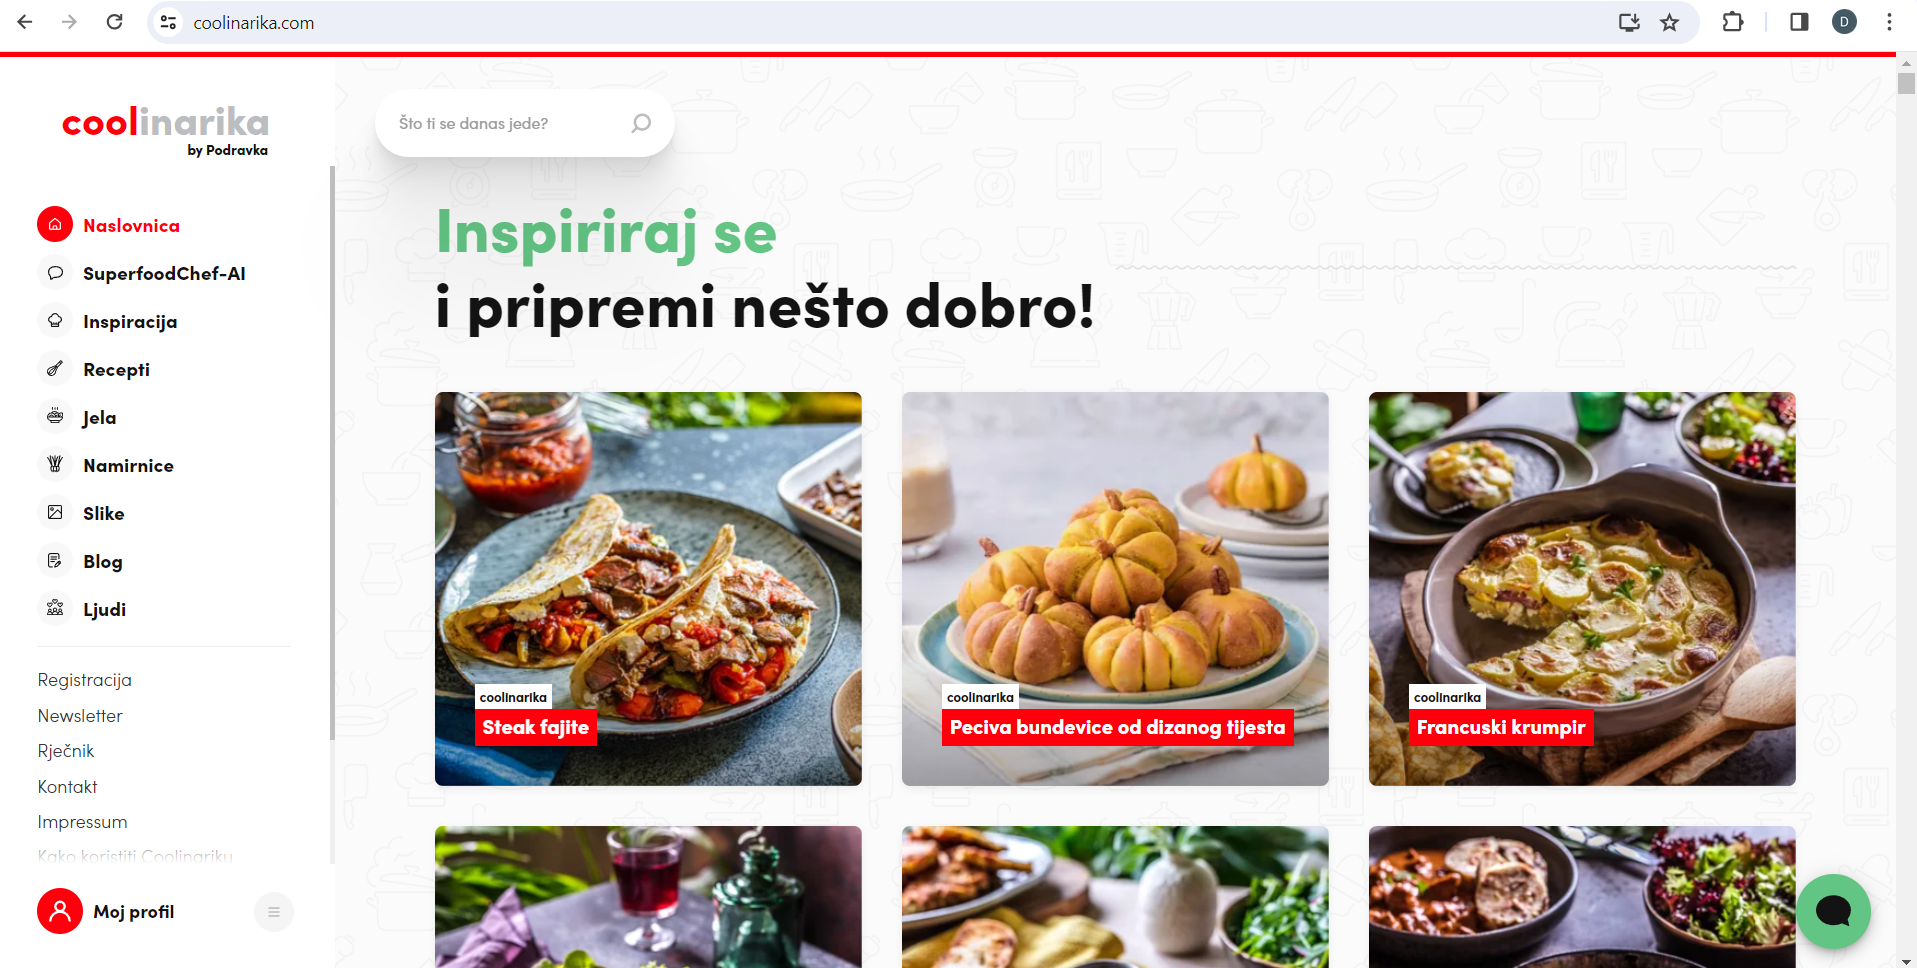
\includegraphics[scale=0.4]{slike/coolinarika.PNG} %veličina slike u odnosu na originalnu datoteku i pozicija slike
			\centering
			\caption{Sučelje platforme coolinarika}
			\label{coolinarika}
		\end{figure}
	
		\begin{figure}[H]
			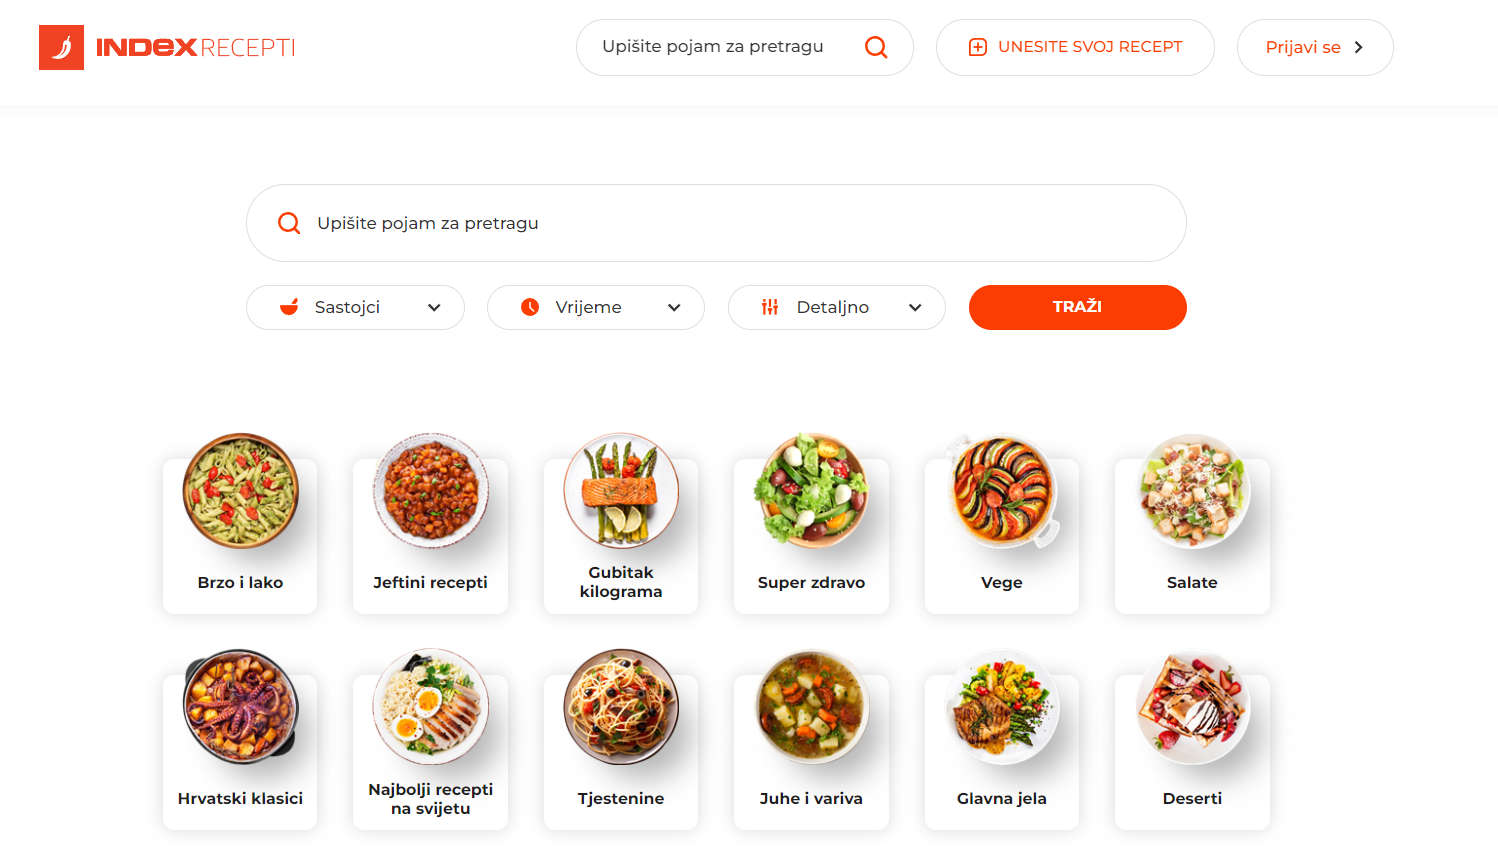
\includegraphics[scale=0.4]{slike/indexRecepti.PNG} %veličina slike u odnosu na originalnu datoteku i pozicija slike
			\centering
			\caption{Sučelje platforme Index Recepti}
			\label{indexRecepti}
		\end{figure}
		
		\section{Skup korisnika koji bi mogao biti zainteresiran za ostvareno rješenje}
		
		Za ovakvo rješenje mogli bi biti zainteresirani putni entuzijasti. Uz minimalne promjene platforme njezina tema bi se mogla promijeniti. Za temu putovanja promijenili bi recepte u mjesta koje bi ljudi mogli posjetiti. Tako bi umjesto sastojaka, uputstava i ostalih koraka vezano za kuhanje, korisnici sada vidjeli znamenitosti određenog mjesta, parkove prirode ili nacionalne parkove u blizini i dodatne zanimljivosti koje bi bilo vrijedno pogledati. Kuharica bi sada bila regija ili država, a korisnici bi se dijelili na putopisce, kulturologe i avanturiste. Kulturolozi bi zamijenili kulinarske entuzijaste i mogli bi stvarati svoje "kuharice" tj. najbolja mjesta za posjetiti u određenoj regiji. Putopisci bi zamijenili nutricioniste, i umjesto "dijete" mogli bi korisnicima predložiti personaliziranu rutu ovisno o tome koje regije sve žele posijetiti i koji su njihovi interesi,odnosno u kojim dijelovima tih regija bi najviše mogli uživati. Klijenti bi ovdje bili avanturisti, ljudi koji žele putovati i na ovoj platformi traže ideje za mjesta vrijedna posjeta, kao i mogući putni vodič.
		
		\section{Opseg projektnog zadatka}
		Na platformi KuhajIT postoji opcija registracije.
		Neregistrirani korisnik može poslati zahtjev za registraciju u kojoj navodi i za koju se ulogu želi prijaviti. Moguće uloge su:
		\begin{packed_item}
		    \item klijent
		    \item kulinarski entuzijast
		    \item nutricionist
		\end{packed_item}
		
		Ako se neregistrirani korisnik želi prijaviti kao klijent, potrebno mu je sljedeće:
		\begin{packed_item}
			\item korisničko ime
			\item lozinka
			\item ime korisnika
			\item prezime korisnika
		\end{packed_item}
		
		Međutim, ako se neregistrirani korisnik želi prijaviti kao kulinarski entuzijast ili nutricionist, potrebno je još:
		\begin{packed_item}
			\item slika
			\item kratka biografija
			\item email
		\end{packed_item}
		
		Kako bi neregistrirani korisnik postao kulinarski entuzijast ili nutricionist na platformi KuhajIT, kao takvog ga mora potvrditi ADMINISTRATOR.
				Svi su registrirani korisnici, bili oni klijenti, kulinarski entuzijasti ili nutricionisti, u mogućnosti mijenjati podatke unutar svog KuhajIT profila. Neregistrirani korisnici nemaju tu mogućnost iz jednostavnog razloga što nisu registrirani, stoga ne posjeduju račun čije bi podatke mogli mijenjati.
	Svi korisnici, bili oni registrirani ili neregistrirani, mogu pretraživati i pregledavati recepte koje su objavili kulinarski entuzijasti. Na platformi postoji i mogućnost ostavljanja recenzija i ocjena na recepte i kuharice, koje mogu ostaviti svi korisnici, a autor recepta (kulinarski entuzijast koji je objavio recept) ima mogućnost odgovoriti na recenzije korisnika. Ako recenziju ostavi neregistrirani korisnik, on se vodi kao anoniman.
	Zadatak nutricionista je da unosi informacije o proizvodima (sastojcima jela), razvrstava ih u kategorije s oznakama te na temelju dostupnih informacijama o proizvodima izrađuje dijete za klijente i kulinarske entuzijaste platforme KuhajIT.
	Informacije o nutritivnim vrijednostima svakog proizvoda definirane su na 100g, a uključuju sljedeće:
	\begin{packed_item}
		\item energija
		\item masnoće
		\item zasićene masne kiseline
		\item ugljikohidrati
		\item šećeri
		\item bjelančevine
		\item sol
	\end{packed_item}
	
	Osim navedenog, svaki proizvod mora imati i priloženu fotografiju, masu i neke dodatke oznake koje ga svrstavaju u različite kategorije. Neke od dodatnih oznaka su:
		\begin{packed_item}
			\item "sadrži kikiriki"
			\item "sadrži gluten
			\item "riba"
			\item "tjestenina"
		\end{packed_item}
	
	Dijeta, koju nutricionist stvara, personalizirana je klijentu. Ona se može definirati s ograničenjima na određene proizvode, kategorije proizvoda, proizvode s nedopuštenim količinama sastojaka, te dnevnim limitom za određene nutritivne vrijednosti proizvoda. Dijeta sadrži i opis od nutricionista koji ju je stvorio.
	Kuharice su skupine recepata koje stvaraju kulinarski entuzijasti i nose tematski naziv, primjerice "Variva". Stvaranjem kuharice u njoj se ne nalazi niti jedan recept, a recepte u kuharice također dodaju njihovi autori, kulinarski entuzijasti. Međutim, to je opcionalno, odnosno ne mora svaki recept biti u pripadnoj kuharici, no isto tako, jedan recept može biti u više različitih kuharica istog kulinarskog entuzijasta. Tako se, primjerice, recept za varivo od graška može nalaziti u kuharici "Brzi ručkovi", a istovremeno i u kuharici "Priprema jela unaprijed". Valja napomenuti da je kulinarski entuzijast koji stvara kuharicu i sprema recepte u nju sam odgovoran za tematsku povezanost recepata u kuharici. Tako kulinarski entuzijast u kuharicu "Brzi ručkovi" teoretski može staviti i recept za čokoladnu tortu.
	Svaki recept je napisan po istom kalupu: najprije su navedeni svi potrebni sastojci, zajedno s njihovom količinom,i ukupno vrijeme kuhanja, zatim slijede koraci pripreme jela, popraćeni slikama koje pobliže objašnjavaju postupak. Naposljetku je navedena veličina jedne porcije jela uz popratnu sliku gotovog jela.
	Klijent platforme može skenirati bar kodove sastojaka, ili, ako neki od sastojaka nema bar kod, unijeti ga ručno iz dostupnih kategorija, koje ima doma i pomoću kojih želi pripremiti jelo, a na temelju tih sastojaka i ograničenja koje postavlja dijeta registriranog korisnika, platforma će pronaći i poredati recepte po njihovoj prihvatljivosti. Nakon što klijent odabere i pripremi odabrano jelo, on ga može označiti kao pripravljenog u tom danu, na temelju čega se, kroz dulji vremenski period, generira statistika konzumiranih nutritivnih vrijednosti u tom periodu.
	Neregistriranim se korisnicima prilikom otvaranja početne stranice prikazuju najnovije kuharice objavljene od strane kulinarskih entuzijasta. S druge strane,  registriranim korisnicima se na početnoj stranici prikazuju isprobani recepti, informacije o dijeti koju prate, nove kuharice i recepti od kulinarskih entuzijasta koje prate
	
		\section{Moguće nadogradnje projektnog zadatka}
		Neke od mogućih nadogradnji projektnog zadatka za platformu KuhajIT uključuju:
	\begin{packed_item}
		\item dodavanje video recepata
		\item chat u kojemu se registrirani korisnici mogu dopisivati s nutricionistima, kulinarskim entuzijastima i ostalima
		\item obavještavanje korisnika kada neki od kulinarskih entuzijasta koje prate objave novi recept ili kuharicu
		\item mogućnost ispisa željenog recepta
		\item "explore" dio na početnoj stranici registriranih korisnika, u kojem mogu otkriti neke nove kulinarske entuzijaste koji objavljuju recepte koji bi im se mogli svidjeti
		\item povezanost platforme s nekom internetskom trgovinom za kupnju namirnica, primjerice "Konzum Klik"
	\end{packed_item}

	\chapter{Specifikacija programske potpore}
		
	\section{Funkcionalni zahtjevi}
			
			\textbf{\textit{dio 1. revizije}}\\
			
			\noindent \textbf{Dionici:}
			
			\begin{packed_enum}
				\item Administrator
				\item Razvojni tim
				\item Svi zainteresirani za kvalitetnu prehranu
			\end{packed_enum}
			
			\noindent \textbf{Aktori i njihovi funkcionalni zahtjevi:}
			
			\begin{packed_enum}
				\item  \underbar{Neregistrirani korisnik (inicijator) može:}
				
				\begin{packed_enum}
					
					\item pretraživati i pregledavati profile kulinarskih entuzijasta te njihove recepte i kuharice
					\item ostaviti anonimnu recenziju i ocjenu na recept
					\item poslati zahtjev za registraciju na platformu
					
				\end{packed_enum}
			
				\item  \underbar{Klijent (inicijator) može:}
		
				\begin{packed_enum}
					
					\item mijenjati podatke na svom korisničkom profilu
					\item pretraživati i pregledavati profile kulinarskih entuzijasta te njihove recepte i kuharice
					\item ostaviti recenziju i ocjenu na recept pod svojim korisničkim imenom
					\item unositi proizvode koje ima doma i koji su spremni za uporabu u receptu
						\begin{packed_enum}
							\item skeniranjem bar koda
							\item ručnim unosom iz dostupnih kategorija
						\end{packed_enum}
					\item zatražiti od nutricionista da im složi dijetu
					\item označiti koje su recepte konzumirali u kojem danu
					
				\end{packed_enum}
				
				\item \underbar{Kulinarski entuzijast (inicijator) može:}
				\begin{packed_enum}
					\item obavljati iste akcije kao i klijent
					\item stvarati nove tematske kuharice i u njima recepte
				\end{packed_enum}
				
				\item \underbar{Nutricionist (sudionik) može:}
				\begin{packed_enum}
					
					\item obavljati iste akcije kao i klijent
					\item izrađivati dijete na temelju dostupnih informacija o proizvodima
					\item unositi podatke o proizvodima
					\item razvrstavati proizvode u kategorije s oznakama
				\end{packed_enum}
				
				\item \underbar{Administrator (incijator) može:}
				\begin{packed_enum}
					\item potvrditi zahtjev za registraciju korisnika koji se želi registrirati kao kulinarski entuzijast ili nutricionist
					\item vidjeti popis svih registriranih korisnika i njihovih osobnih podataka
					\item brisati recenzije koje su u suprotnosti s pravilima korištenja aplikacije 
				\end{packed_enum}
					
				
			\end{packed_enum}
			
			\eject 
			
			
				
			\subsection{Obrasci uporabe}
				
				\textbf{\textit{dio 1. revizije}}
				
				\subsubsection{Opis obrazaca uporabe}
						
					\noindent \underbar{\textbf{UC1 - Zahtjev za registraciju}}
					\begin{packed_item}
	
						\item \textbf{Glavni sudionik: Korisnik}
						\item  \textbf{Cilj: Stvoriti korisnički profil}
						\item  \textbf{Sudionici: Baza podataka, administrator}
						\item  \textbf{Preduvjet: - } 
						\item  \textbf{Opis osnovnog tijeka:}
						
						\item[] \begin{packed_enum}
	
							\item Korisnik odabire za koju se ulogu želi registrirati
							\item Korisnik unosi podatke potrebne za registraciju
							\item Korisnik šalje zahtjev za registraciju
							\item Korisnik dobiva potvrdu od administratora da je uspješno registriran
						\end{packed_enum}
						
						\item  \textbf{Opis mogućih odstupanja:}
						
						\item[] \begin{packed_item}
	
							\item[2.a] email ili korisničko ime koje je korisnik unio je već zauzeto ili u krivom obliku
							\item[] \begin{packed_enum}
								
								\item Sustav obavještava korisnika o neuspjelom upisu i vraća ga na stranicu za registraciju
								\item Korisnik mijenja potrebne podatke te zavrsava unos ili odustaje od
registracije		
							\end{packed_enum}
							
							\item[3.a] uvjeti za registraciju korisnika kao kulinarskog entuzijasta ili nutricionista nisu zadovoljeni
							\item[] \begin{packed_enum}
								
								\item Sustav obavještava korisnika o neuspjelom upisu i vraća ga na stranicu za registraciju
								\item Korisnik mijenja potrebne podatke te zavrsava unos ili odustaje od
registracije		
							\end{packed_enum}
							
						\end{packed_item}
					\end{packed_item}
					
					
					\noindent \underbar{\textbf{UC2 - Prijava u sustav}}
					\begin{packed_item}
	
						\item \textbf{Glavni sudionik: Klijent}
						\item  \textbf{Cilj: Uspješno se prijaviti u sustav}
						\item  \textbf{Sudionici: Baza podataka}
						\item  \textbf{Preduvjet: Registracija } 
						\item  \textbf{Opis osnovnog tijeka:}
						
						\item[] \begin{packed_enum}
	
							\item Korisnik unosi podatke za prijavu
					
							\item Potvrda o ispravnosti unesenih podataka
							\item Pristup korisničkim funkcijama
						\end{packed_enum}
						
						\item  \textbf{Opis mogućih odstupanja:}
						
						\item[] \begin{packed_item}
	
							\item[1.a] Neispravni podaci za prijavu
							\item[] \begin{packed_enum}
								
								\item Sustav obavještava korisnika o neuspjeloj prijavi i vraća ga na stranicu za prijavu		
							\end{packed_enum}
						\end{packed_item}
					\end{packed_item}
					
					\noindent \underbar{\textbf{UC3 - Promjena osobnih podataka}}
					\begin{packed_item}
	
						\item \textbf{Glavni sudionik: Klijent}
						\item  \textbf{Cilj: Promijeniti željene osobne podatke}
						\item  \textbf{Sudionici: Baza podataka}
						\item  \textbf{Preduvjet: Prijava } 
						\item  \textbf{Opis osnovnog tijeka:}
						
						\item[] \begin{packed_enum}
	
							\item Korisnik odabire opciju za promjenu podataka
					
							\item Korisnik mijenja željene podatke
							\item Korisnik sprema promjene
							\item Baza podataka se ažurira
						\end{packed_enum}
						
						\item  \textbf{Opis mogućih odstupanja:}
						
						\item[] \begin{packed_item}
	
							\item[3.a] Korisnik ne spremi promjene
							\item[] \begin{packed_enum}
								
								\item Sustav obavještava korisnika da nije spremio podatke prije izlaska
iz prozora
								
							\end{packed_enum}
						\end{packed_item}
					\end{packed_item}
					
					
					\noindent \underbar{\textbf{UC4 - Pretraživanje profila kulinarskih entuzijasta}}
					\begin{packed_item}
	
						\item \textbf{Glavni sudionik: Korisnik}
						\item  \textbf{Cilj: Pretražiti profile kulinarskih entuzijasta}
						\item  \textbf{Sudionici: Baza podataka}
						\item  \textbf{Preduvjet: - } 
						\item  \textbf{Opis osnovnog tijeka:}
						
						\item[] \begin{packed_enum}
	
							\item Korisnik u tražilicu upisuje kategoriju po kojoj želi pretraživati
					
							\item Na ekran se izlistavaju profili koji odgovaraju upisanoj kategoriji

						\end{packed_enum}
					\end{packed_item}
									
					
					\noindent \underbar{\textbf{UC5 - Ostavljanje recenzije na recept}}
					\begin{packed_item}
	
						\item \textbf{Glavni sudionik: Korisnik}
						\item  \textbf{Cilj: Ostaviti recenziju na recept}
						\item  \textbf{Sudionici: Baza podataka}
						\item  \textbf{Preduvjet: - } 
						\item  \textbf{Opis osnovnog tijeka:}
						
						\item[] \begin{packed_enum}
	
							\item Korisnik odabire recept na kojem želi ostaviti recenziju
					
							\item Korisnik ostavlja ocjenu ili recenziju na odabrani recept
						\end{packed_enum}
					\end{packed_item}
					
					\noindent \underbar{\textbf{UC6 - Odgovor autora na recenziju}}
					\begin{packed_item}
	
						\item \textbf{Glavni sudionik: Kulinarski entuzijast}
						\item  \textbf{Cilj: Odgovoriti na recenziju koju je na recept kulinarskog entuzijasta ostavio drugi korisnik}
						\item  \textbf{Sudionici: Baza podataka}
						\item  \textbf{Preduvjet: Prijava } 
						\item  \textbf{Opis osnovnog tijeka:}
						
						\item[] \begin{packed_enum}
	
							\item Kulinarski entuzijast odabere recept na kojem je ostavljena recenzija
							\item Kulinarski entuzijast odabere opciju odgovora na recenziju
							\item Kulinarski entuzijast odgovara na recenziju
							\item Kulinarski entuzijast objavljuje odgovor na recenziju
						\end{packed_enum}
					\end{packed_item}
					
					
					
			\noindent \underbar{\textbf{UC7 - Stvaranje nove kuharice}}
					\begin{packed_item}
	
						\item \textbf{Glavni sudionik: Kulinarski entuzijast}
						\item  \textbf{Cilj: Stvoriti novu tematsku kuharicu}
						\item  \textbf{Sudionici: Baza podataka}
						\item  \textbf{Preduvjet: Prijava } 
						\item  \textbf{Opis osnovnog tijeka:}
						
						\item[] \begin{packed_enum}
	
							\item Kulinarski entuzijast odabire opciju za stvaranje nove kuharice
							\item Kulinarski entuzijast stvara novu kuharicu 
							\item Baza podataka se ažurira
						\end{packed_enum}
					\end{packed_item}
					
					
					\noindent \underbar{\textbf{UC8 - Stvaranje novog recepta}}
					\begin{packed_item}
	
						\item \textbf{Glavni sudionik: Kulinarski entuzijast}
						\item  \textbf{Cilj: Stvoriti novi recept}
						\item  \textbf{Sudionici: Baza podataka}
						\item  \textbf{Preduvjet: Prijava } 
						\item  \textbf{Opis osnovnog tijeka:}
						
						\item[] \begin{packed_enum}
	
							\item Kulinarski entuzijast odabire opciju za stvaranje novog recepta
							\item Kulinarski entuzijast unosi sve potrebne podatke za stvaranje novog recepta
							\item Kulinarski entuzijast stvara novi recept
							\item Baza podataka se ažurira
						\end{packed_enum}
					\end{packed_item}
					
					
					\noindent \underbar{\textbf{UC9 - Dodavanje recepta u kuharicu}}
					\begin{packed_item}
	
						\item \textbf{Glavni sudionik: Kulinarski entuzijast}
						\item  \textbf{Cilj: Dodati recept u kuharicu koja mu tematski odgovara}
						\item  \textbf{Sudionici: Baza podataka}
						\item  \textbf{Preduvjet: Prijava } 
						\item  \textbf{Opis osnovnog tijeka:}
						
						\item[] \begin{packed_enum}
	
							\item Kulinarski entuzijast odabire recept koji želi dodati u kuharicu
							\item Kulinarski entuzijast odabire opciju dodavanja recepta u kuharicu
							\item Kulinarski entuzijast iz prikazane liste dostupnih kuharica odabire onu u koju želi dodati recept
							\item Kulinarski entuzijast dodaje recept u odabranu kuharicu
							\item Baza podataka se ažurira
						\end{packed_enum}
					\end{packed_item}
					
					
					\noindent \underbar{\textbf{UC10 - Brisanje kuharice}}
					\begin{packed_item}
	
						\item \textbf{Glavni sudionik: Kulinarski entuzijast}
						\item  \textbf{Cilj: Obrisati kuharicu}
						\item  \textbf{Sudionici: Baza podataka}
						\item  \textbf{Preduvjet: Prijava } 
						\item  \textbf{Opis osnovnog tijeka:}
						
						\item[] \begin{packed_enum}
	
							\item Kulinarski entuzijast odabire kuharicu koju želi obrisati
							\item Kulinarski entuzijast briše odabranu kuharicu, no ne i recepte koji se nalaze u njoj
							\item Baza podataka se ažurira
						\end{packed_enum}
					\end{packed_item}
					

					\noindent \underbar{\textbf{UC11 - Brisanje recepta iz baze}}
					\begin{packed_item}
	
						\item \textbf{Glavni sudionik: Kulinarski entuzijast}
						\item  \textbf{Cilj: Obrisati recept iz svih kuharica i baze}
						\item  \textbf{Sudionici: Baza podataka}
						\item  \textbf{Preduvjet: Prijava } 
						\item  \textbf{Opis osnovnog tijeka:}
						
						\item[] \begin{packed_enum}
	
							\item Kulinarski entuzijast odabire recept koji želi obrisati
							\item Kulinarski entuzijast briše odabrani recept
							\item Baza podataka se ažurira
						\end{packed_enum}
					\end{packed_item}
					
					\noindent \underbar{\textbf{UC12 - Brisanje recepta iz pojedine kuharice}}
					\begin{packed_item}
	
						\item \textbf{Glavni sudionik: Kulinarski entuzijast}
						\item  \textbf{Cilj: Obrisati recept iz samo jedne kuharice}
						\item  \textbf{Sudionici: Baza podataka}
						\item  \textbf{Preduvjet: Prijava } 
						\item  \textbf{Opis osnovnog tijeka:}
						
						\item[] \begin{packed_enum}
	
							\item Kulinarski entuzijast odabire kuharicu iz koje želi obrisati recept
							\item Kulinarski entuzijast odabire recept koji želi obrisati
							\item Kulinarski entuzijast briše recept iz kuharice
							\item Baza podataka se ažurira
						\end{packed_enum}
					\end{packed_item}
					
					
					\noindent \underbar{\textbf{UC13 - Skeniranje bar koda proizvoda}}
					\begin{packed_item}
	
						\item \textbf{Glavni sudionik: Klijent}
						\item  \textbf{Cilj: Unos proizvoda }
						\item  \textbf{Sudionici: Baza podataka}
						\item  \textbf{Preduvjet: Prijava } 
						\item  \textbf{Opis osnovnog tijeka:}
						
						\item[] \begin{packed_enum}
	
							\item Klijent odabire opciju skeniranja bar koda proizvoda kojeg ima doma
							\item Klijent skenira proizvod
							\item Baza podataka se ažurira
						\end{packed_enum}

					\item  \textbf{Opis mogućih odstupanja:}
						
						\item[] \begin{packed_item}
	
							\item[2.a] Bar kod se ne može očitati
							\item[] \begin{packed_enum}
								
								\item Sustav obavještava korisnika da je skeniranje bar koda neuspješno i da pokuša ponovno ili ručno unese proizvod	
							\end{packed_enum}
						\end{packed_item}
					\end{packed_item}
					
					
				\noindent \underbar{\textbf{UC14 - Ručni unos proizvoda}}
					\begin{packed_item}
	
						\item \textbf{Glavni sudionik: Klijent}
						\item  \textbf{Cilj: Unos proizvoda }
						\item  \textbf{Sudionici: Baza podataka}
						\item  \textbf{Preduvjet: Prijava } 
						\item  \textbf{Opis osnovnog tijeka:}
						
						\item[] \begin{packed_enum}
	
							\item Klijent odabire opciju ručnog unosa proizvoda kojeg ima doma
							\item Klijent ručno unosi proizvod
							\item Baza podataka se ažurira
						\end{packed_enum}

					\item  \textbf{Opis mogućih odstupanja:}
						
						\item[] \begin{packed_item}
	
							\item[2.a] Proizvod nije prepoznat
							\item[] \begin{packed_enum}
								
								\item Sustav obavještava korisnika da proizvod nije prepoznat
							\end{packed_enum}
						\end{packed_item}
					\end{packed_item}
					
					
				\noindent \underbar{\textbf{UC15- Unos podataka o proizvodu}}
					\begin{packed_item}
	
						\item \textbf{Glavni sudionik: Nutricionist}
						\item  \textbf{Cilj: Unos podataka o proizvodu }
						\item  \textbf{Sudionici: Baza podataka}
						\item  \textbf{Preduvjet: Prijava } 
						\item  \textbf{Opis osnovnog tijeka:}
						
						\item[] \begin{packed_enum}
	
							\item Nutricionist odabire opciju unosa podataka o proizvodu
							\item Nutricionist unosi sve potrebne podatke o proizvodu
							\item Nutricionist odabire kojoj kategoriji proizvod pripada
							\item Baza podataka se ažurira
						\end{packed_enum}

					\item  \textbf{Opis mogućih odstupanja:}
						
						\item[] \begin{packed_item}
	
							\item[2.a] Nutricionist nije unio neki od podataka
							\item[] \begin{packed_enum}
								
								\item Sustav obavještava nutricionista da nije unio sve potrebne podatke i vraća ga na stranicu za unos podataka o proizvodu
							\end{packed_enum}
						\end{packed_item}
					\end{packed_item}
					
					
				\noindent \underbar{\textbf{UC16 - Označivanje recepta kao konzumiranog u određenom danu}}
					\begin{packed_item}
	
						\item \textbf{Glavni sudionik: Klijent}
						\item  \textbf{Cilj: Generiranje statistike konzumiranih nutritivnih vrijednosti kroz vrijeme na temelju informacija o tome koji je recept konzumiran koji dan }
						\item  \textbf{Sudionici: Baza podataka}
						\item  \textbf{Preduvjet: Prijava } 
						\item  \textbf{Opis osnovnog tijeka:}
						
						\item[] \begin{packed_enum}
	
							\item Klijent odabire recept koji je konzumirao
							\item Klijent odabire opciju odabira datuma kada je odabrani recept konzumiran
							\item Klijent unosi datum konzumiranja odabranog recepta
							\item Baza podataka se ažurira
						\end{packed_enum}
					\end{packed_item}
					
				\noindent \underbar{\textbf{UC17 - Brisanje proizvoda}}
					\begin{packed_item}
	
						\item \textbf{Glavni sudionik: Nutricionist}
						\item  \textbf{Cilj: Brisanje proizvoda iz baze podataka }
						\item  \textbf{Sudionici: Baza podataka}
						\item  \textbf{Preduvjet: Prijava } 
						\item  \textbf{Opis osnovnog tijeka:}
						
						\item[] \begin{packed_enum}
	
							\item Nutricionist pregledava kategorije proizvoda
							\item Nutricionist odabire kategoriju proizvoda kojeg želi obrisati
							\item Nutricionist odabire proizvod iz odabrane kategorije
							\item Nutricionist briše odabrani proizvod
							\item Baza podataka se ažurira
							\item Otvara se stranica s pregledom svih kategorija proizvoda
						\end{packed_enum}
					\end{packed_item}
					
				\noindent \underbar{\textbf{UC18 - Brisanje korisničkog računa}}
					\begin{packed_item}
	
						\item \textbf{Glavni sudionik: Klijent}
						\item  \textbf{Cilj: Obrisati svoj korisnički račun }
						\item  \textbf{Sudionici: Baza podataka}
						\item  \textbf{Preduvjet: Prijava } 
						\item  \textbf{Opis osnovnog tijeka:}
						
						\item[] \begin{packed_enum}
	
							\item Klijent pregledava osobne podatke
							\item Klijent odabire opciju brisanja korisničkog računa
							\item Klijent briše svoj korisnički račun
							\item Baza podataka se ažurira
							\item Otvara se stranica za registraciju
						\end{packed_enum}
					\end{packed_item}
					
			
			\noindent \underbar{\textbf{UC19 - Slanje zahtjeva za izradu dijete}}
				\begin{packed_item}
				
					\item \textbf{Glavni sudionik: Klijent}
					\item \textbf{Cilj: Dobiti personaliziranu dijetu od nutricionista}
					\item \textbf{Sudionici: Baza podataka}
					\item \textbf{Preduvjet: Prijava}
					\item \textbf{Opis osnovnog tijeka:}
					
					\item[] \begin{packed_enum}
						\item Klijent odabire opciju izrade personalizirane dijete
						\item Klijent upisuje sva ograničenja na proizvode koja želi u dijeti
						\item Klijent šalje zahtjev za izradom dijete
						\item Nutricionist mu šalje personaliziranu dijetu
					\end{packed_enum}
				\end{packed_item}
				
				\noindent \underbar{\textbf{UC20 - Potvrda zahtjeva za registracijom}}
					\begin{packed_item}
	
						\item \textbf{Glavni sudionik: Administrator}
						\item  \textbf{Cilj: Odobriti registraciju kulinarskog entuzijasta ili nutricionista}
						\item  \textbf{Sudionici: Baza podataka}
						\item  \textbf{Preduvjet: Autorizacija} 
						\item  \textbf{Opis osnovnog tijeka:}
						
						\item[] \begin{packed_enum}
	
							\item Administrator odabire zahtjev za registraciju koji želi pregledati
					
							\item Ako su uneseni podatci zadovoljavajući, administrator potvrđuje zahjtev za registracijom
						\end{packed_enum}
						
						\item  \textbf{Opis mogućih odstupanja:}
						
						\item[] \begin{packed_item}
	
							\item[1.a] Neispravni podaci za registraciju
							\item[] \begin{packed_enum}
								
								\item Administrator odbija zahtjev, a sustav obavještava korisnika o neuspjeloj registraciji
							\end{packed_enum}
						\end{packed_item}
					\end{packed_item}
					
					\noindent \underbar{\textbf{UC21 - Prikaz popisa registriranih korisnika i njihovih podataka}}
					\begin{packed_item}
	
						\item \textbf{Glavni sudionik: Administrator}
						\item  \textbf{Cilj: Pristupiti podatcima svih registriranih korisnika}
						\item  \textbf{Sudionici: Baza podataka}
						\item  \textbf{Preduvjet: Autorizacija } 
						\item  \textbf{Opis osnovnog tijeka:}
						
						\item[] \begin{packed_enum}
	
							\item Adiministrator šalje upit u bazu za podatcim svih registriranih korisnika
					
							\item Administrator dobiva popis svih podataka.
						\end{packed_enum}
					\end{packed_item}
					
					\noindent \underbar{\textbf{UC22 - Brisanje recenzija}}
					\begin{packed_item}
	
						\item \textbf{Glavni sudionik: Administrator}
						\item  \textbf{Cilj: Ukloniti recenzije koje su u suprotnosti s pravilima korištenja aplikacije}
						\item  \textbf{Sudionici: Baza podataka}
						\item  \textbf{Preduvjet: Autorizacija } 
						\item  \textbf{Opis osnovnog tijeka:}
						
						\item[] \begin{packed_enum}
	
							\item Adiministrator odabire recenziju koju treba obrisati
					
							\item Administrator briše odabranu recenziju
							\item Baza podataka se ažurira
						\end{packed_enum}
					\end{packed_item}
					
					
									
				\subsubsection{Dijagrami obrazaca uporabe}
					
				\begin{figure}[H]
			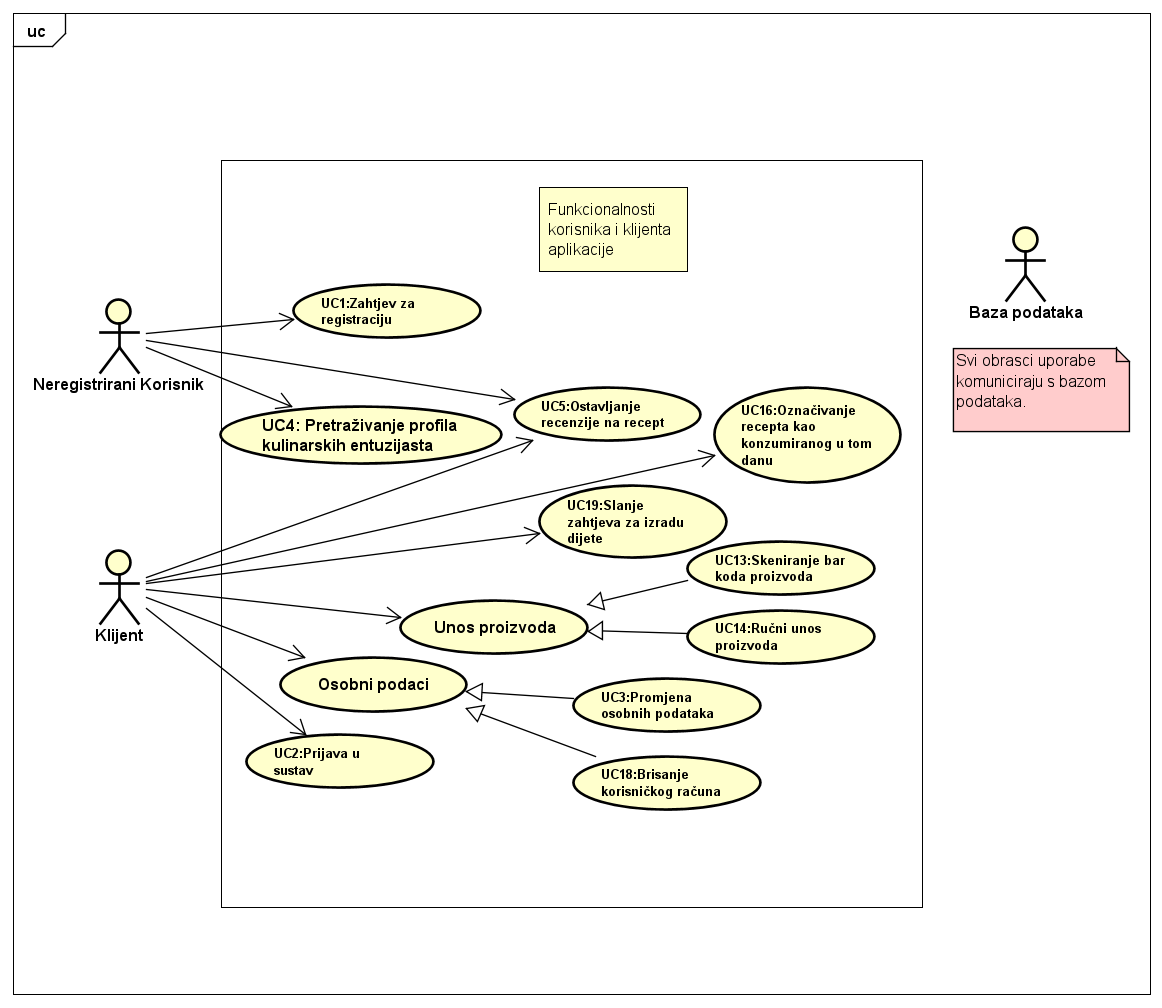
\includegraphics[scale=0.4]{dijagrami/UML_Korisnik_Klijent.png} %veličina slike u odnosu na originalnu datoteku i pozicija slike
			\centering
			\caption{Funkcionalnosti korisnika i klijenta aplikacije}
			\label{UML1}
		\end{figure}
		
		
				\begin{figure}[H]
			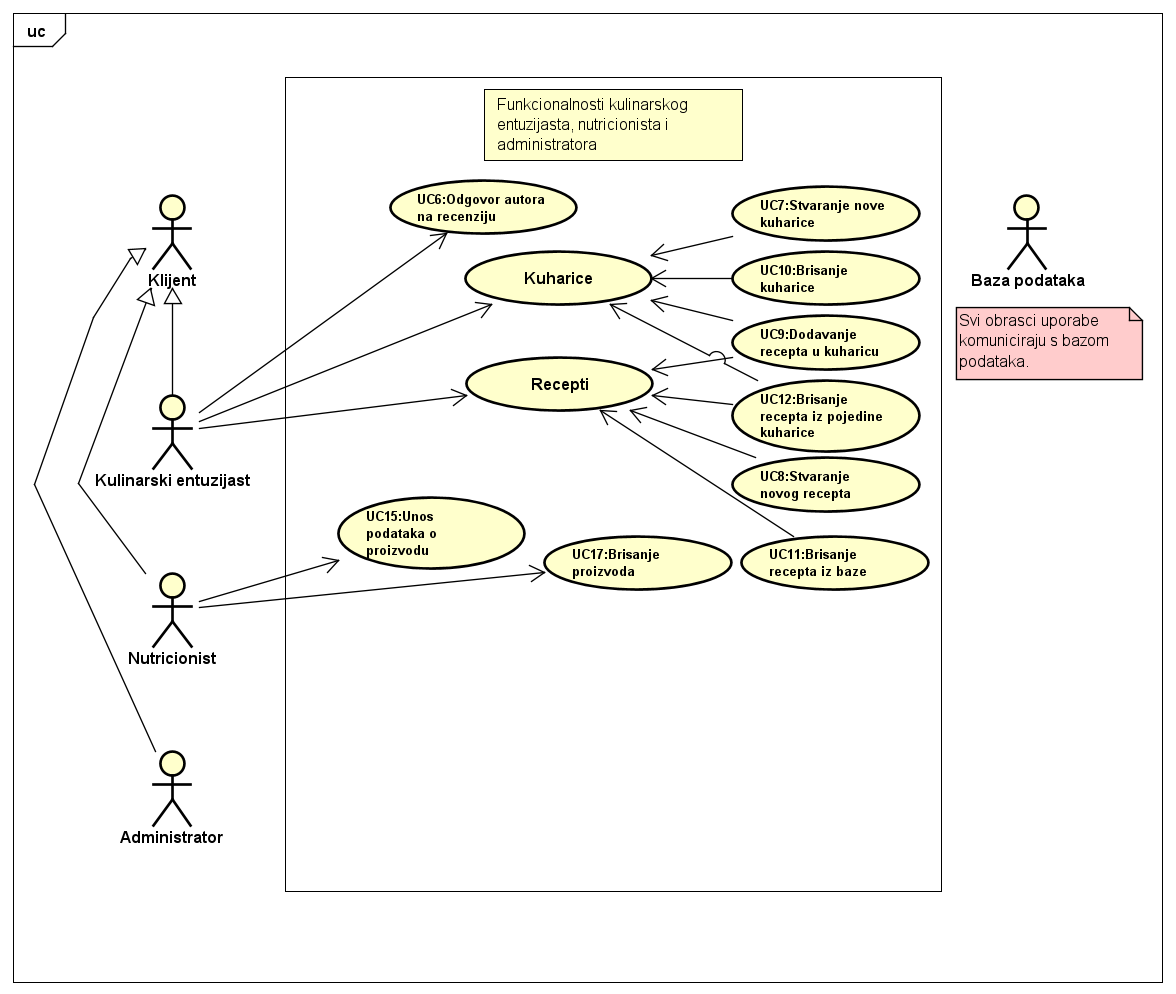
\includegraphics[scale=0.4]{dijagrami/UML_KulinarskiEntuzijast_Nutricionist_Admin.png} %veličina slike u odnosu na originalnu datoteku i pozicija slike
			\centering
			\caption{Funkcionalnosti kulinarskog entuzijasta, nutricionista i administratora aplikacije}
			\label{UML2}
		\end{figure}
				
			\subsection{Sekvencijski dijagrami}
				
				\textbf{\textit{dio 1. revizije}}\\
				
				\begin{large}{\textbf{Obrazac uporabe UC4 - Pretraživanje profila kulinarskih entuzijasta}}\end{large}
				
				Korisnik šalje zahtjev za pretragom profila kulinarskih entuzijasta. Poslužitelj mu omogućava pristup i pretragu. Korisnik u tražilicu upisuje kategoriju po kojoj želi pretražiti kulinarske entuzijaste. Poslužitelj iz baze dohvaća sve kulinarske entuzijaste koji odgovaraju upisanoj kategoriji i prikazuje ih korisniku.
				
					
				\begin{figure}[H]
			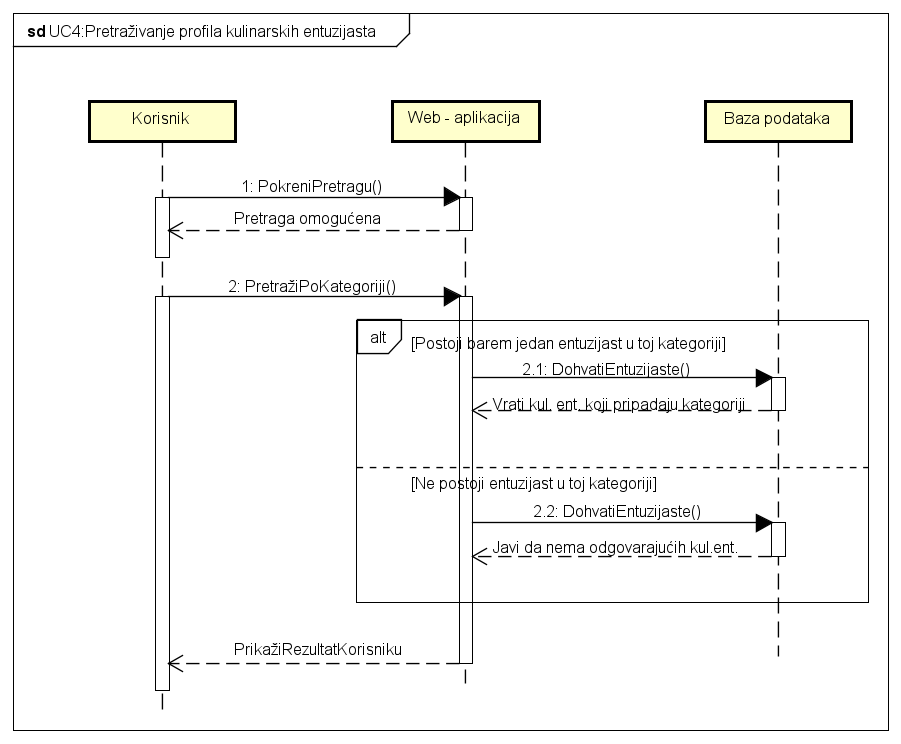
\includegraphics[scale=0.4]{dijagrami/SEQ_UC4.png} %veličina slike u odnosu na originalnu datoteku i pozicija slike
			\centering
			\caption{Sekvencijski dijagram za UC4}
			\label{SEQ_UC4}
		\end{figure}
	

				\begin{large}{\textbf{Obrazac uporabe UC8 - Stvaranje novog recepta}}\end{large}
				
				Kulinarski entuzijast šalje zahtjev za stvaranjem novog recepta. Poslužitelj mu omogućava pristup i stvaranje novog recepta. Kulinarski entuzijast upisuje sve podatke potrebne za stvaranje novog recepta: potrebne sastojke i njihovu količinu, korake pripreme, veličinu porcije, vrijeme kuhanja i galeriju popratnih slika. Nakon potvrde podataka, poslužitelj unosi novi recept u bazu podataka.
				
					
				\begin{figure}[H]
			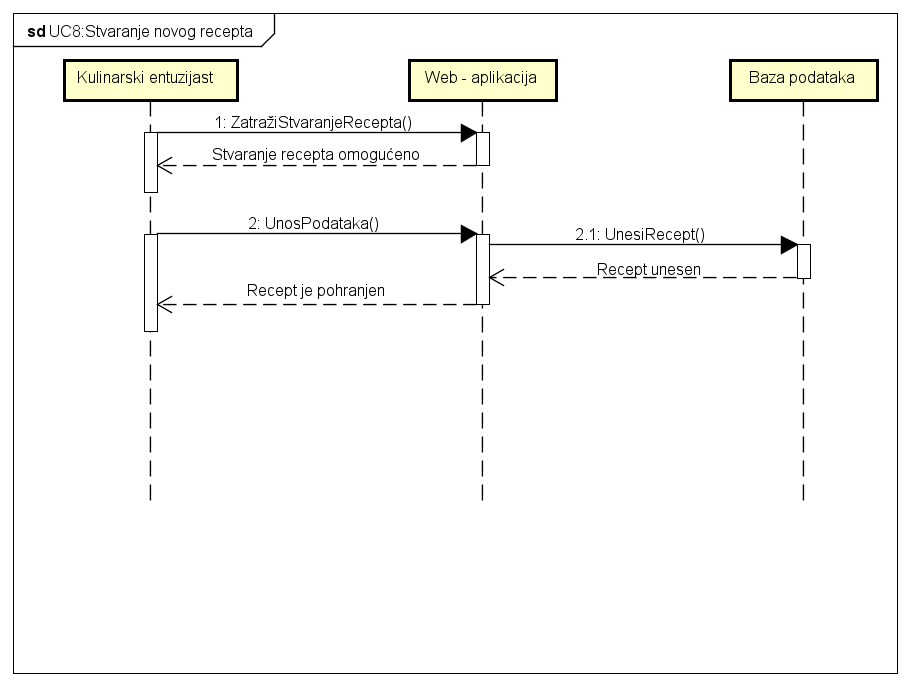
\includegraphics[scale=0.4]{dijagrami/SEQ_UC8.png} %veličina slike u odnosu na originalnu datoteku i pozicija slike
			\centering
			\caption{Sekvencijski dijagram za UC8}
			\label{SEQ_UC8}
		\end{figure}
				
			\begin{large}{\textbf{Obrazac uporabe UC13 - Skeniranje bar koda proizvoda}}\end{large}

			Klijent šalje zahtjev za skeniranjem bar koda proizvoda kojeg ima doma. Poslužitelj mu omogućava pristup i skeniranje bar koda proizvoda. Klijent skenira bar kod proizvoda, i ako je bar kod čitljiv i proizvod prepoznat, poslužitelj unosi skenirani proizvod u bazu podataka.
				
					
				\begin{figure}[H]
			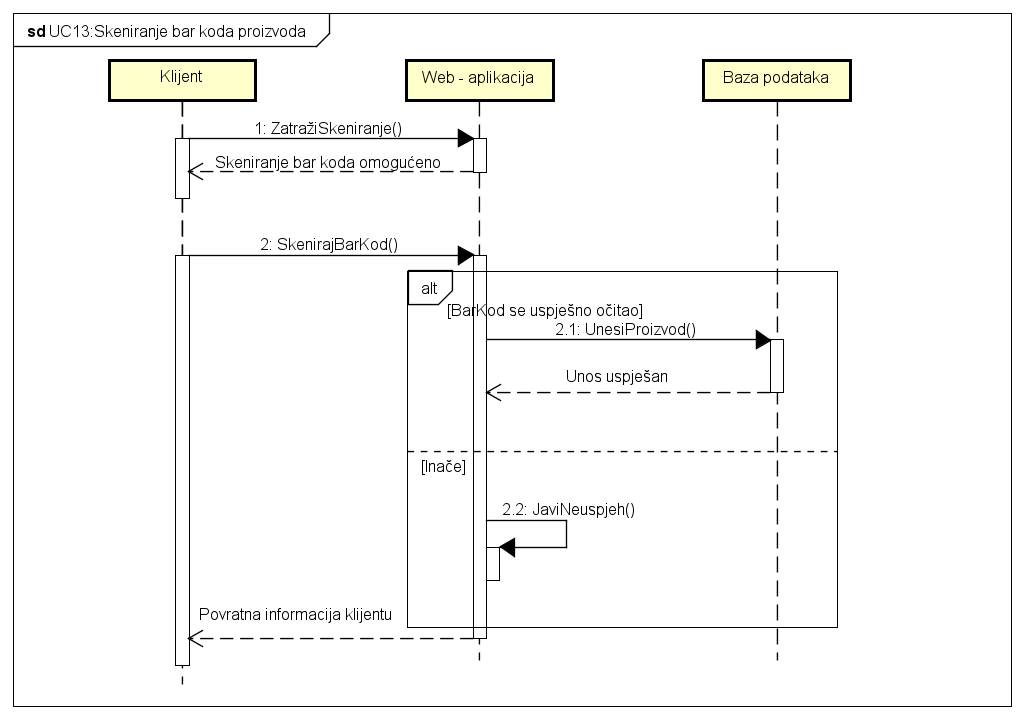
\includegraphics[scale=0.4]{dijagrami/SEQ_UC13.png} %veličina slike u odnosu na originalnu datoteku i pozicija slike
			\centering
			\caption{Sekvencijski dijagram za UC13}
			\label{SEQ_UC13}
		\end{figure}
				
			\begin{large}{\textbf{Obrazac uporabe UC14 - Ručni unos proizvoda}}\end{large}
			
			Klijent šalje zahtjev za ručnim unosom proizvoda kojeg ima doma. Poslužitelj mu omogućava pristup i unos proizvoda. Klijent unosi podatke o proizvodu ručno, primjerice njegov naziv, naziv proizvođača, masu, energetsku vrijednost itd. Nakon potvrde unosa, poslužitelj unosi novi recept u bazu podataka.
				
					
				\begin{figure}[H]
			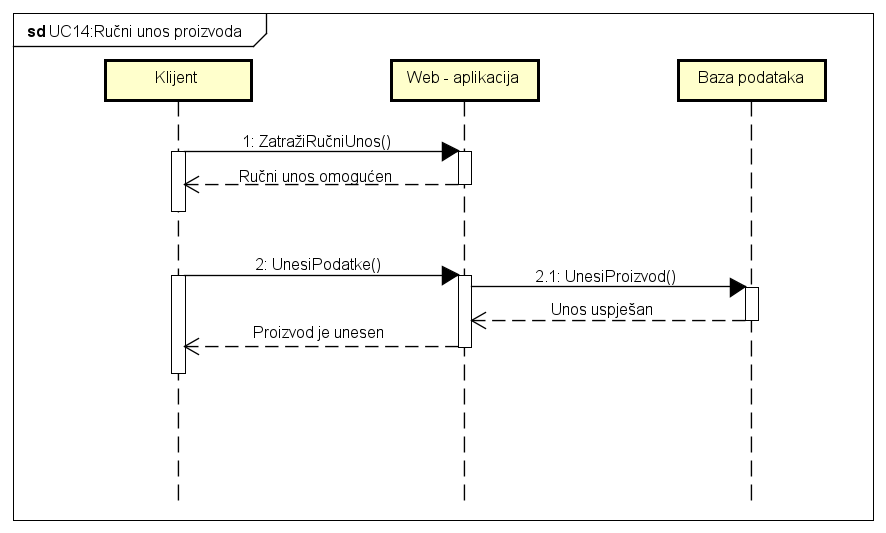
\includegraphics[scale=0.4]{dijagrami/SEQ_UC14.png} %veličina slike u odnosu na originalnu datoteku i pozicija slike
			\centering
			\caption{Sekvencijski dijagram za UC14}
			\label{SEQ_UC14}
		\end{figure}

		\section{Ostali zahtjevi}

			\begin{itemize}
			\item Sustav treba podržavati rad više korisnika u stvarnom vremenu.
			\item Sustav treba implementirati kao web aplikaciju koristeći objektno-orijentirane jezike.
			\item Sustav mora biti prilagođena veličini ekrana na kojem je prikazana.
			\item Sustav mora biti u potpunosti responzivan, bez dugog čekanja na podatke.
			\item Sustav mora biti što jednostavniji i prilagođeniji korisniku za korištenje.
			\item Sustav mora podržavati znakove hrvatske abecede pri unosu i prikazu sadržaja.
			\item Sustav mora imati omogućen pristup iz javne mreže.
			\item Sustav mora biti otporan na neispravno korištenje korisničkog sučelja, u smislu da neispravno korištenje ne smije narušiti njegovu funkcionalnost.
			\item Sustav mora ograničiti korisnika na pristup jedino onim resursima kojima ima pristup.
			\end{itemize}

			 
			 
	
	\chapter{Arhitektura i dizajn sustava}
	
	Za ostvarenje naše aplikacije odabrali smo arhitekturu zasnovanu na događajima. Prednosti ovog tipa arhitekture su mnoge: 
	\begin{itemize}
		\item svaki od servisa arhitekture može biti neovisan entitet, što povećava fleksibilnost 
		\item događaji se mogu pratiti u stvarnom vremenu, što olakšava analizu sustava
		\item događaji predstavljaju promjene stanja pa je komponentama omogućeno da reagiraju na te promjene
	\end{itemize}
	
				\begin{figure}[H]
			\includegraphics[scale=0.4]{slike/event\_driven\_architecture.PNG} %veličina slike u odnosu na originalnu datoteku i pozicija slike
			\centering
			\caption{Prikaz arhitekture zasnovane na događajima}
			\label{event_driven_architecture}
		\end{figure}
		
	Specifično, radi se o MVC (Model-View-Controller) obrascu, koji odvaja korisničko sučelje od ostatka sustava. On dodatno smanjuje međuovisnost U/I sučelja i ostatka sustava. Sastoji se od tri dijela:
	
		\begin{itemize}
			\item model - sadrži razrede čiji se objekti obrađuju
			\item view (pogled) - sadrži razrede čiji objekti služe za prikaz podataka (korisničko sučelje)
			\item controller (nadglednik) - sadrži razrede koji upravljaju i rukuju korisničkom interakcijom s pogledom i modelom
		\end{itemize}
		
			\begin{figure}[H]
			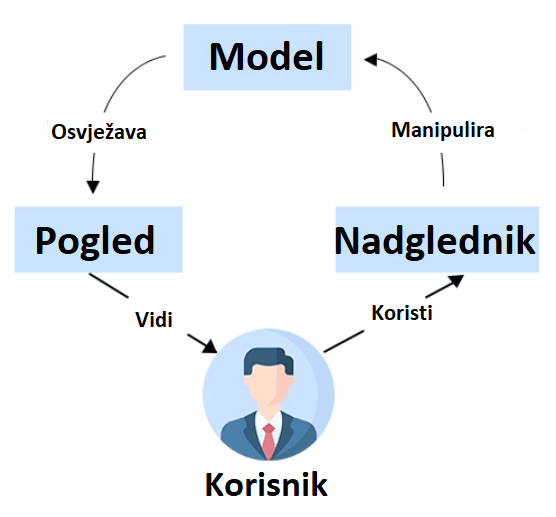
\includegraphics[scale=0.4]{slike/mvc.PNG} %veličina slike u odnosu na originalnu datoteku i pozicija slike
			\centering
			\caption{Prikaz načina rada MVC obrasca}
			\label{mvc}
		\end{figure}
		
	Po principu oblikovanja arhitekture odabrali smo \textit{Podijeli pa vladaj} arhitekturu, kako bismo se unutar tima mogli podijeliti u manje timove koji rade na određenim problemima i kako bismo, ako to bude bilo potrebno, jednostavno zamijenili željene dijelove bez opsežne intervencije u cijeli sustav.
	
			\begin{figure}[H]
			\includegraphics[scale=0.4]{slike/divide\_and\_conquer.PNG} %veličina slike u odnosu na originalnu datoteku i pozicija slike
			\centering
			\caption{Prikaz principa djelovanja "podijeli pa vladaj"}
			\label{divide_and_conquer}
		\end{figure}
		
	Arhitektura našeg sustava dijeli se na tri komponente:
	\begin{itemize}
		\item Web preglednik - softverska aplikacija koja omogućuje korisnicima pregledavanje i interakciju sa svim sadržajima Interneta. Glavna funkcija web preglednika je prikazivanje web stranica koje su oblikovane u obliku programskog koda na korisniku jasan način. Neki poznati web-preglednici uključuju Google Chrome, Mozilla Firefox, Opera...Web preglednik služi i kao medijator između korisnika, koji šalje zahtjeve, i web poslužitelja, koji prima zahtjeve i na njih odgovara.
		\item Web poslužitelj - program koji prosljeđuje web sadržaje web klijentu/pregledniku na njegov zahtjev putem protokola HTTP
		\item Baza podataka - omogućuje organiziranu pohranu podataka koje je potrebno pohraniti (za KuhajIT su to podaci o korisničkim profilima, recepti, kuharice, osvrti na recepte, proizvodi i ostali)
	\end{itemize}
			
		\section{Baza podataka}

		Za ostvarenje naše aplikacije KuhajIT odabrali smo relacijsku bazu podataka PostgreSQL, koja svojom jednostavnom i lako razumljivom strukturom olakšava pregled i upravljanje podacima. Ključne komponente relacijske baze podataka su entiteti (tablice okarakterizirane imenom i skupom atributa) te veze među entitetima (strukture koje povezuju podatke iz različitih entiteta pomoću ključeva).
		
		Entiteti naše baze podataka su:
		\begin{itemize}
			\item User
			\item Recipe
			\item Recipe Ingredient
			\item Ingredient
			\item Cookbook
			\item Cookbook Recipe
			\item Review
			\item Response
			\item Image
		\end{itemize}
		
		
			\subsection{Opis tablica}
				
				\textbf{User} Entitet \textit{User} sadrži atribute važne za svakog registriranog korisnika aplikacije KuhajIT. Ti atributi su: ID korisnika, korisničko ime, lozinku, ime, prezime, email, uloga, biografija, url osobne fotografije i oznaka potvrđenosti. U vezi je \textit{One-to-Many} s entitetom \textit{Review} preko korisničkog ID-ja, \textit{One-to-Many} s entitetom \textit{Cookbook} preko korisničkog ID-ja, \textit{Recipe} preko korisničkog ID-ja i \textit{One-to-Many} s entitetom \textit{Response} preko korisničkog ID-ja.
				
				\begin{longtblr}[
					label=none,
					entry=none
					]{
						width = \textwidth,
						colspec={|X[6,l]|X[6, l]|X[20, l]|}, 
						rowhead = 1,
					} %definicija širine tablice, širine stupaca, poravnanje i broja redaka naslova tablice
					\hline \SetCell[c=3]{c}{\textbf{User}}	 \\ \hline[3pt]
					\SetCell{LightGreen}id & INT	&  	ID korisnika, sekvencijski generiran.  	\\ \hline
					username 	& VARCHAR &  Korisničko ime korisnika, koje mora biti jedinstveno, korisnik si ga bira sam pri registraciji, no može ga promijeniti. 	\\ \hline 
					password & VARCHAR & Lozinka za pristup korisničkom računu. \\
\hline
					name & VARCHAR	&  	Ime korisnika	\\ \hline 
					surname & VARCHAR & Prezime korisnika \\
\hline
					role & VARCHAR & Uloga koju neregistrirani korisnik želi imati (nutricionist, kulinarski entuzijast ili klijent). \\
\hline

					email & VARCHAR &   Ako se korisnik želi registrirati kao kulinarski entuzijast/nutricionist, mora priložiti email, inače atribut poprima NULL vrijednost.\\ \hline 
					slika & VARCHAR & Ako se korisnik želi registrirati kao kulinarski entuzijast/nutricionist, mora priložiti osobnu fotografiju, čiji se URL sprema u bazu, inače atribut poprima NULL vrijednost.\\
\hline

					biografija & VARCHAR & Ako se korisnik želi registrirati kao kulinarski entuzijast/nutricionist, mora priložiti kratku biografiju, inače atribut poprima NULL vrijednost.\\
\hline
				\end{longtblr}
				
				\textbf{Recipe} Entitet \textit{Recipe} sadrži atribute važne za svaki recept objavljen na web aplikaciji KuhajIT. Ti atributi su: ID recepta, ime recepta, vrijeme pripreme, koraci pripreme, ID autora recepta i veličina porcije. U vezi je \textit{One-to-Many} s entitetom \textit{Image} preko ID-ja recepta, \textit{One-to-Many} s entitetom \textit{Cookbook Recipe} preko ID-ja recepta, \textit{One-to-Many} s entitetom \textit{Recipe Ingredient} preko ID-ja recepta i \textit{Many-to-One} s entitetom \textit{User} preko ID-ja korisnika.
				
					\begin{longtblr}[
					label=none,
					entry=none
					]{
						width = \textwidth,
						colspec={|X[8,l]|X[6, l]|X[20, l]|}, 
						rowhead = 1,
					} %definicija širine tablice, širine stupaca, poravnanje i broja redaka naslova tablice
					\hline \SetCell[c=3]{c}{\textbf{Recipe}}	 \\ \hline[3pt]
					\SetCell{LightGreen}id & INT	&  Jedinstveni	ID recepta, sekvencijski generiran.  	\\ 
\hline
					cook\_time 	& INT &  Vrijeme pripreme recepta. 	\\ 
\hline 
					portion\_size & INT & Veličina porcije pripremljenog recepta. \\
\hline
					steps\_of\_making & VARCHAR	&  Koraci pripreme recepta.	\\ 
\hline 
					\SetCell{LightBlue}creator\_id	& INT &   Korisnički ID autora recepta.	\\ 
\hline 
				\end{longtblr}
				
				\textbf{Recipe Ingredient} Entitet \textit{Recipe Ingredient} sadrži atribute važne za pohranu sastojaka koji se koriste u pojedinom receptu objavljenom na web aplikaciji KuhajIT. Ti atributi su: ID sastojka recepta, količina sastojka, ID recepta i ID sastojka. U vezi je \textit{Many-to-One} s entitetom \textit{Recipe} preko ID-ja recepta i \textit{Many-to-One} s entitetom \textit{Ingredient}.
				
				\begin{longtblr}[
					label=none,
					entry=none
					]{
						width = \textwidth,
						colspec={|X[6,l]|X[6, l]|X[20, l]|}, 
						rowhead = 1,
					} %definicija širine tablice, širine stupaca, poravnanje i broja redaka naslova tablice
					\hline \SetCell[c=3]{c}{\textbf{Recipe Ingredient}}	 \\ \hline[3pt]
					\SetCell{LightGreen}id & INT	&  Jedinstveni ID sastojka recepta, sekvencijski generiran.  	\\ \hline
					quantity & INT &  Količina sastojka potrebnog za recept. 	\\ \hline 
					\SetCell{LightBlue}ingredient\_id	& INT &   ID sastojka.	\\ \hline
					\SetCell{LightBlue}recipe\_id	& INT & ID recepta. \\ \hline
				\end{longtblr}
				
				\textbf{Ingredient} Entitet \textit{Ingredient} sadrži atribute važne za svaki sastojak.
Ti atributi su: ID sastojka i ime sastojka. U vezi je \textit{One-to-Many} s entitetom \textit{Recipe Ingredient} preko ID-ja sastojka.

				\begin{longtblr}[
					label=none,
					entry=none
					]{
						width = \textwidth,
						colspec={|X[6,l]|X[6, l]|X[20, l]|}, 
						rowhead = 1,
					} %definicija širine tablice, širine stupaca, poravnanje i broja redaka naslova tablice
					\hline \SetCell[c=3]{c}{\textbf{Ingredient}}	 \\ \hline[3pt]
					\SetCell{LightGreen}id & INT	&  Jedinstveni ID sastojka, sekvencijski generiran.  	\\ \hline
					name 	& VARCHAR &  Naziv sastojka. 	\\ \hline 
				\end{longtblr}	
				
				\textbf{Cookbook} Entitet \textit{Cookbook} sadrži atribute važne za svaku kuharicu stvorenu od kulinarskog entuzijasta na web aplikaciji KuhajIT.
Ti atributi su: id kuharice, kategorija kuharice, naziv kuharice i id autora. U vezi je \textit{One-to-Many} s entitetom \textit{Cookbook Recipe} preko ID-ja kuharice i \textit{Many-to-One} s entitetom \textit{User} preko ID-ja korisnika (kulinarskog entuzijasta koji ju je stvorio).

				\begin{longtblr}[
					label=none,
					entry=none
					]{
						width = \textwidth,
						colspec={|X[6,l]|X[6, l]|X[20, l]|}, 
						rowhead = 1,
					} %definicija širine tablice, širine stupaca, poravnanje i broja redaka naslova tablice
					\hline \SetCell[c=3]{c}{\textbf{Cookbook}}	 \\ \hline[3pt]
					\SetCell{LightGreen}id & INT	&  Jedinstveni ID kuharice, sekvencijski generiran.  	\\ \hline
					category 	& VARCHAR &  Kategorija kuharice. 	\\ \hline 
					
					name & VARCHAR & Naziv kuharice. \\ \hline
					\SetCell{LightBlue}creator\_id	& INT &   Korisnički ID autora kuharice.	\\ \hline 
					
				\end{longtblr}
				
		\textbf{Cookbook Recipe} Entitet \textit{Cookbook Recipe} sadrži atribute važne za pohranu recepata u pojedinu kuharicu na web aplikaciji KuhajIT.
Ti atributi su: ID kuharice i ID recepta. U vezi je \textit{Many-to-One} s entitetom \textit{Cookbook} preko ID-ja kuharice i \textit{Many-to-One} s entitetom \textit{Recipe} preko ID-ja recepta koji se u kuharici nalazi.

			\begin{longtblr}[
					label=none,
					entry=none
					]{
						width = \textwidth,
						colspec={|X[6,l]|X[6, l]|X[20, l]|}, 
						rowhead = 1,
					} %definicija širine tablice, širine stupaca, poravnanje i broja redaka naslova tablice
					\hline \SetCell[c=3]{c}{\textbf{Cookbook Recipe}}	 \\ \hline[3pt]
					\SetCell{LightGreen}cookbook\_id & INT	&  ID kuharice.  	\\ \hline
					\SetCell{LightGreen}recipe\_id 	& INT &  ID recepta. 	\\ \hline				
				\end{longtblr}
				
				\textbf{Review} Entitet \textit{Review} sadrži atribute važne za svaku recenziju ostavljenu na recept na web aplikaciji KuhajIT.
Ti atributi su: ID recenzije, ocjena recepta dodijeljena u recenziji, poruka ostavljena u recenziji, ID autora recenzije i ID recepta na koji je recenzija ostavljena. U vezi je \textit{One-to-Many} s entitetom \textit{Cookbook Recipe} preko ID-ja kuharice i \textit{Many-to-One} s entitetom \textit{User} preko ID-ja korisnika koji je ostavio recenziju, \textit{Many-to-One} s entitetom \textit{Recipe} preko ID-ja recepta na koji je recenzija ostavljena i \textit{One-to-Many} s entitetom \textit{Response} preko ID-ja recenzije.

\begin{longtblr}[
					label=none,
					entry=none
					]{
						width = \textwidth,
						colspec={|X[6,l]|X[6, l]|X[20, l]|}, 
						rowhead = 1,
					} %definicija širine tablice, širine stupaca, poravnanje i broja redaka naslova tablice
					\hline \SetCell[c=3]{c}{\textbf{Review}}	 \\ \hline[3pt]
					\SetCell{LightGreen}id & INT	&  Jedinstveni ID recenzije, sekvencijski generiran.  	\\ \hline
					mark 	& INT &  Ocjena ostavljena u recenziji. 	\\ \hline 
					
					message & VARCHAR & Poruka ostavljena u recenziji. \\ \hline
					\SetCell{LightBlue}creator\_id & INT &   Korisnički ID autora recenzije, ako je recenziju ostavio neregistrirani korisnik, poprima vrijednost NULL.	\\ \hline 
					\SetCell{LightBlue} recipe\_id & INT &   ID recepta na kojeg je recenzija ostavljena.	\\ \hline 
					
				\end{longtblr}


\textbf{Response} Entitet \textit{Response} sadrži atribute važne za svaki odgovor na recenziju ostavljenu na recept na web aplikaciji KuhajIT.
Ti atributi su: ID odgovora, poruka ostavljena u odgovoru, ID autora odgovora (kulinarski entuzijast na čiji je recept ostavljena recenzija) i ID recenzije na koju je odgovor ostavljen. U vezi je \textit{Many-to-One} s entitetom \textit{Review} preko ID-ja recenzije i \textit{Many-to-One} s entitetom \textit{User} preko ID-ja korisnika koji odgovara na recenziju.
				
			\begin{longtblr}[
					label=none,
					entry=none
					]{
						width = \textwidth,
						colspec={|X[6,l]|X[6, l]|X[20, l]|}, 
						rowhead = 1,
					} %definicija širine tablice, širine stupaca, poravnanje i broja redaka naslova tablice
					\hline \SetCell[c=3]{c}{\textbf{Response}}	 \\ \hline[3pt]
					\SetCell{LightGreen}id & INT	&  Jedinstveni ID odgovora na recenziju, sekvencijski generiran.  	\\ \hline
					message & VARCHAR & Poruka ostavljena u odgovoru na recenziju. \\ \hline
					\SetCell{LightBlue}creator\_id	& INT &   Korisnički ID autora odgovora na recenziju.	\\ \hline 
					\SetCell{LightBlue}review\_id & INT &   ID recenzije na koju autor recepta odgovara.	\\ \hline 
					
				\end{longtblr}
				
				\textbf{Image} Entitet \textit{Image} sadrži atribute važne za svaku fotografiju učitanu u sklopu recepta na web aplikaciji KuhajIT.
Ti atributi su: ID fotografije, URL fotografije i ID recepta uz kojeg je fotografija učitana. U vezi je \textit{Many-to-One} s entitetom \textit{Recipe} preko ID-ja recepta.

				\begin{longtblr}[
					label=none,
					entry=none
					]{
						width = \textwidth,
						colspec={|X[6,l]|X[6, l]|X[20, l]|}, 
						rowhead = 1,
					} %definicija širine tablice, širine stupaca, poravnanje i broja redaka naslova tablice
					\hline \SetCell[c=3]{c}{\textbf{Image}}	 \\ \hline[3pt]
					\SetCell{LightGreen}id & INT	&  Jedinstveni ID učitane fotografije, sekvencijski generiran.  	\\ \hline

					url & VARCHAR & URL učitane fotografije. \\ \hline	
					\SetCell{LightBlue}recipe\_id	& INT &   ID recepta uz koji je fotografija učitana.	\\ \hline 	
				\end{longtblr}
				
				\eject	
	
	  \section{Dijagram razreda}
			
			
			\begin{figure}[H]
			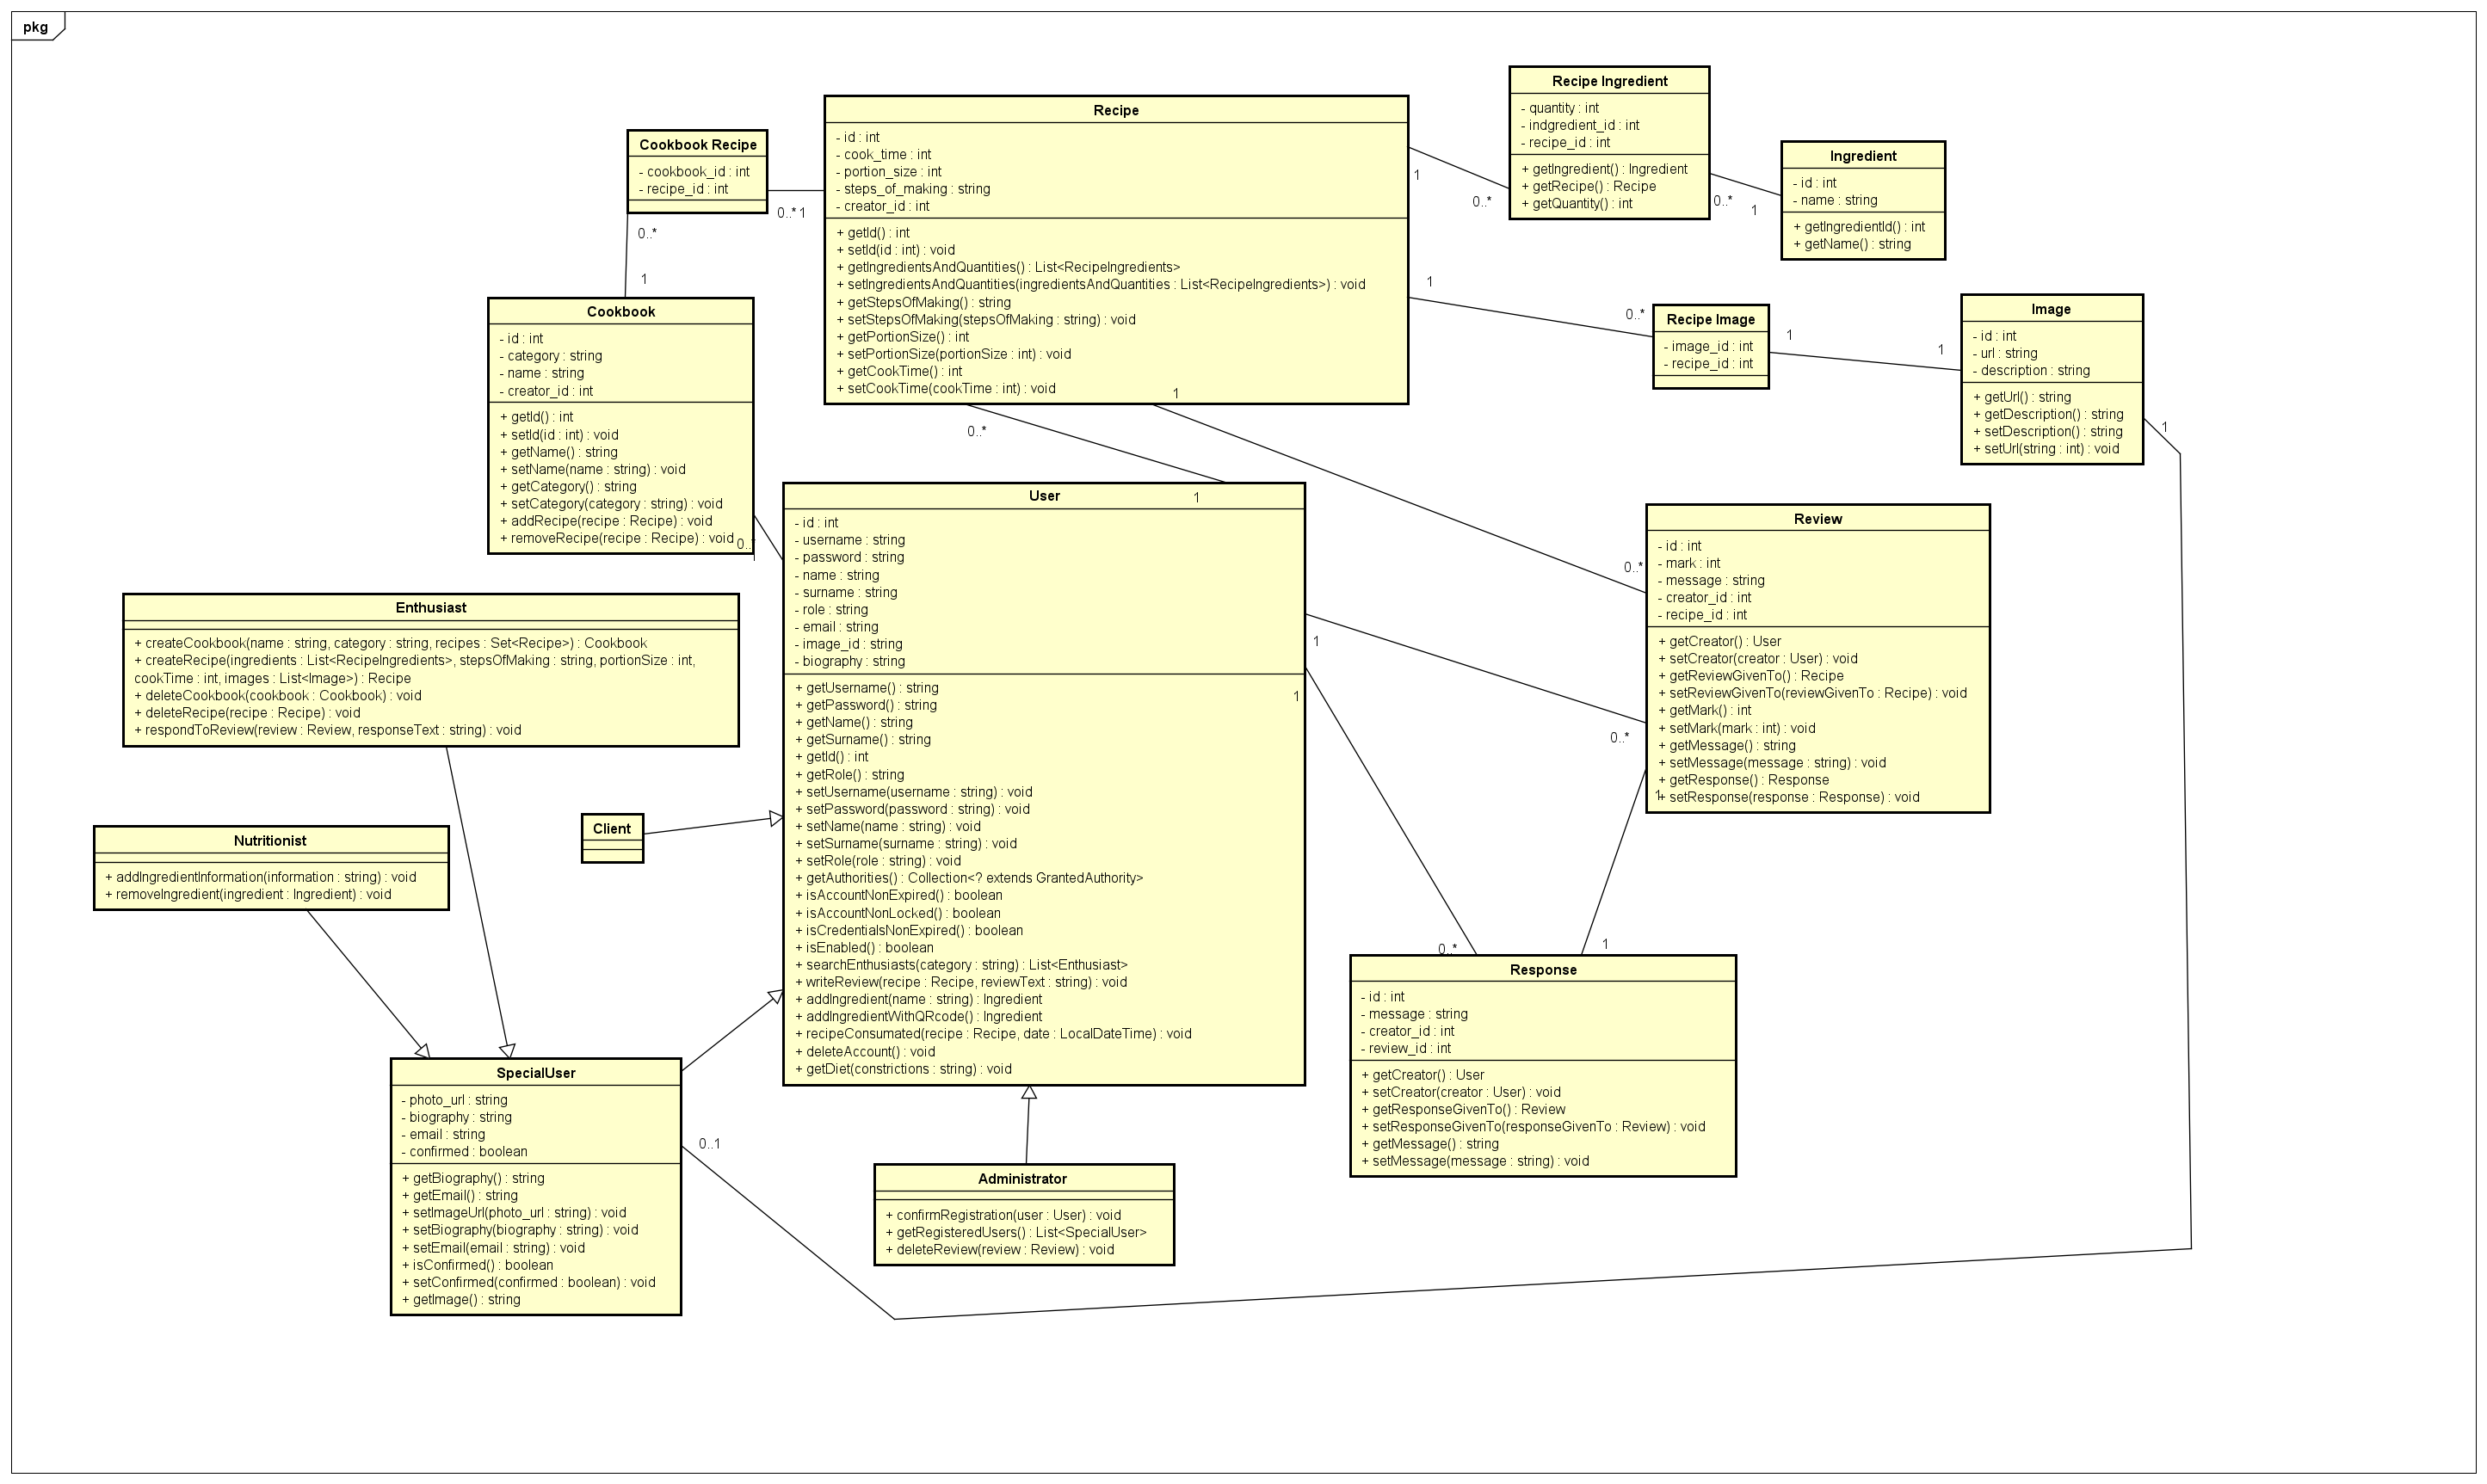
\includegraphics[scale=0.2]{dijagrami/UML_dijagram_razreda_models.png} %veličina slike u odnosu na originalnu datoteku i pozicija slike
			\centering
			\caption{Dijagram razreda - dio Models}
			\label{Dijagram razreda - dio Models}
		\end{figure}
			
			
			\eject 		
			
		\section{Dijagram stanja}
			
			
			\textbf{\textit{dio 2. revizije}}\\
			
			\textit{Potrebno je priložiti dijagram stanja i opisati ga. Dovoljan je jedan dijagram stanja koji prikazuje \textbf{značajan dio funkcionalnosti} sustava. Na primjer, stanja korisničkog sučelja i tijek korištenja neke ključne funkcionalnosti jesu značajan dio sustava, a registracija i prijava nisu. }
			
			
			\eject 
		
		\section{Dijagram aktivnosti}
			
			\textbf{\textit{dio 2. revizije}}\\
			
			 \textit{Potrebno je priložiti dijagram aktivnosti s pripadajućim opisom. Dijagram aktivnosti treba prikazivati značajan dio sustava.}
			
			\eject
		\section{Dijagram komponenti}
		
			\textbf{\textit{dio 2. revizije}}\\
		
			 \textit{Potrebno je priložiti dijagram komponenti s pripadajućim opisom. Dijagram komponenti treba prikazivati strukturu cijele aplikacije.}
	\chapter{Implementacija i korisničko sučelje}
		
		
		\section{Korištene tehnologije i alati}
		
			 Za međusobnu komunikaciju tijekom izrade naše KuhajIT aplikacije korištene su dvije aplikacije: \textcolor{blue}{\underline{\href{https://discord.com/download}{\textcolor{blue}{Discord}}}}\footnote{\url{https://discord.com/download}} i \textcolor{blue}{\underline{\href{https://www.whatsapp.com/download/}{\textcolor{blue}{WhatsApp}}}}\footnote{\url{https://www.whatsapp.com/download/}}.
			 		 
WhatsApp je aplikacija za razmjenu poruka koja omogućava korisnicima slanje tekstualnih poruka, medijskih datoteka (poput slika, videa i audio zapisa), te poziva i video poziva putem internetskog povezivanja. Mi smo ju koristili za interno dogovaranje o onome što je iduće potrebno obaviti te o terminima sastanaka uživo.

Discord je platforma za komunikaciju putem interneta koja je prvobitno dizajnirana za zajednice igrača, ali se brzo proširila na različite druge vrste korisnika. Omogućava korisnicima stvaranje privatnih ili javnih "servera" (prostorija) gdje se mogu razgovarati putem teksta, glasa ili videa. Mi smo ju koristili za hitne sastanke u slučaju da je netko od članova pri izradi naišao na problem bilo kakve vrste i trebala mu je asistencija drugog člana tima.

Upravljanje izvornim kodom ostvareno je sustavom \textcolor{blue}{\underline{\href{https://git-scm.com/downloads}{\textcolor{blue}{Git}}}}\footnote{\url{https://git-scm.com/downloads}}, a udaljeni repozitorij
čitavog projekta dostupan nam je bio na web platformi \textcolor{blue}{\underline{\href{https://github.com/}{\textcolor{blue}{GitHub}}}}\footnote{\url{https://github.com/}}.

			Git je sustav za upravljanje verzijama koji se široko koristi u razvoju softvera. Omogućava programerima i timovima praćenje promjena u izvornom kodu tijekom vremena, praćenje različitih verzija projekta te suradnju među programerima, te smo ga mi na taj način koristili.
			
			GitHub je web platforma za upravljanje verzijama i suradnju na razvoju softvera. Osnovna funkcionalnost GitHub-a leži u Git-u, koji omogućuje razvojnom timu praćenje promjena u izvornom kodu tijekom vremena. 
			Za izradu svih UML dijagrama korišten je alat \textcolor{blue}{\underline{\href{https://astah.net/downloads/}{\textcolor{blue}{Astah UML}}}}\footnote{\url{https://astah.net/downloads/}}.
			
Astah UML je vrsta alata koji pomaže programerima, analitičarima sustava i drugima da vizualiziraju, modeliraju i dokumentiraju arhitekturu softvera. Podržava različite vrste dijagrama, od kojih smo mi koristili dijagrame razreda, stanja, aktivnosti, komponenti, dijagrame obrazaca uporabe te sekvencijske dijagrame.

Odabrana razvojna okruženja pri izradi naše aplikacije bila su \textcolor{blue}{\underline{\href{https://code.visualstudio.com/Download}{\textcolor{blue}{Visual Studio Code}}}}\footnote{\url{https://code.visualstudio.com/Download}} za frontend i \textcolor{blue}{\underline{\href{https://www.eclipse.org/downloads/}{\textcolor{blue}{Eclipse}}}}\footnote{\url{https://www.eclipse.org/downloads/}} za backend.


Visual Studio Code je razvojno okruženje za pisanje koda razvijen od strane Microsofta. Odlikuje ga bogata podrška za web tehnologije, kao što su HTML, CSS, JavaScript, Typescript itd.

Eclipse je razvojno okruženje koje podržava brojne programske jezike, a neki od njih su: Java, C++, PHP, Python, Ruby...

Kako je već prije navedeno, za razvoj frontenda naše aplikacije koristili smo \textcolor{blue}{\underline{\href{https://www.javascript.com/}{\textcolor{blue}{JavaScript}}}}\footnote{\url{https://www.javascript.com/}} i \textcolor{blue}{\underline{\href{https://react.dev/}{\textcolor{blue}{React}}}}\footnote{\url{https://react.dev/}}.

JavaScript je visokoprogamski jezik koji se često koristi za izgradnju dinamičkih web stranica i web aplikacija, razvijen u Netscape Communications Corporation-u. Najčešće se koristi za programiranje na strani klijenta.

React je JavaScript biblioteka za izgradnju korisničkih sučelja, koju karakterizira komponentna arhitektura koja olakšava organizaciju koda i upravljanje stanjem aplikacije.

Za razvoj backenda naše aplikacije korišten je \textcolor{blue}{\underline{\href{https://spring.io/projects/spring-boot/}{\textcolor{blue}{Spring Boot}}}}\footnote{\url{https://spring.io/projects/spring-boot/}}.

Spring Boot je open-source okvir za izgradnju Java web aplikacija i mikroservisa, dio šireg Spring ekosustava. Posebno je fokusiran na pojednostavljenje konfiguracije, ubrzanje razvoja i olakšavanje izgradnje samostalnih aplikacija.


Baza podataka razvijena je pomoću sustava za upravljanje bazom podataka \textcolor{blue}{\underline{\href{https://www.postgresql.org/download/}{\textcolor{blue}{PostgreSQL}}}}\footnote{\url{https://www.postgresql.org/download/}}.
			\eject 
			
		\section{Ispitivanje programskog rješenja}
			
			\subsection{Ispitivanje komponenti}
\textbf{Test 1: Uspješna registracija} \\
Provedeno je testiranje uspješne registracije novog, dotad neregistriranog korinsika u sustav. Registracija je uspješna ako ne baca iznimku i ako metoda "registerUser" klase UserService vraća istinitu vrijednost. Na slikama ispod prikazani su test uspješne registracije i metoda "registerUser" klase UserService, kao i potvrda uspješne provedbe testa.

		\begin{figure}[H]
			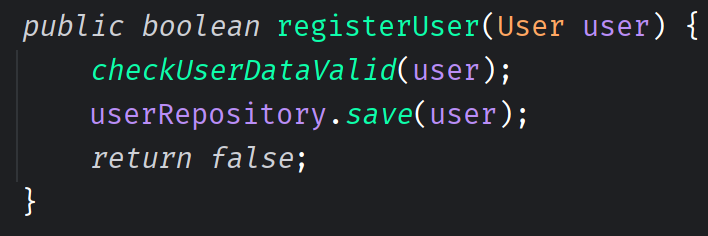
\includegraphics[scale=0.4]{slike/registerUser.PNG} %veličina slike u odnosu na originalnu datoteku i pozicija slike
			\centering
			\caption{Metoda "registerUser" klase UserService}
			\label{Metoda "registerUser" klase UserService}
		\end{figure}
		
				\begin{figure}[H]
			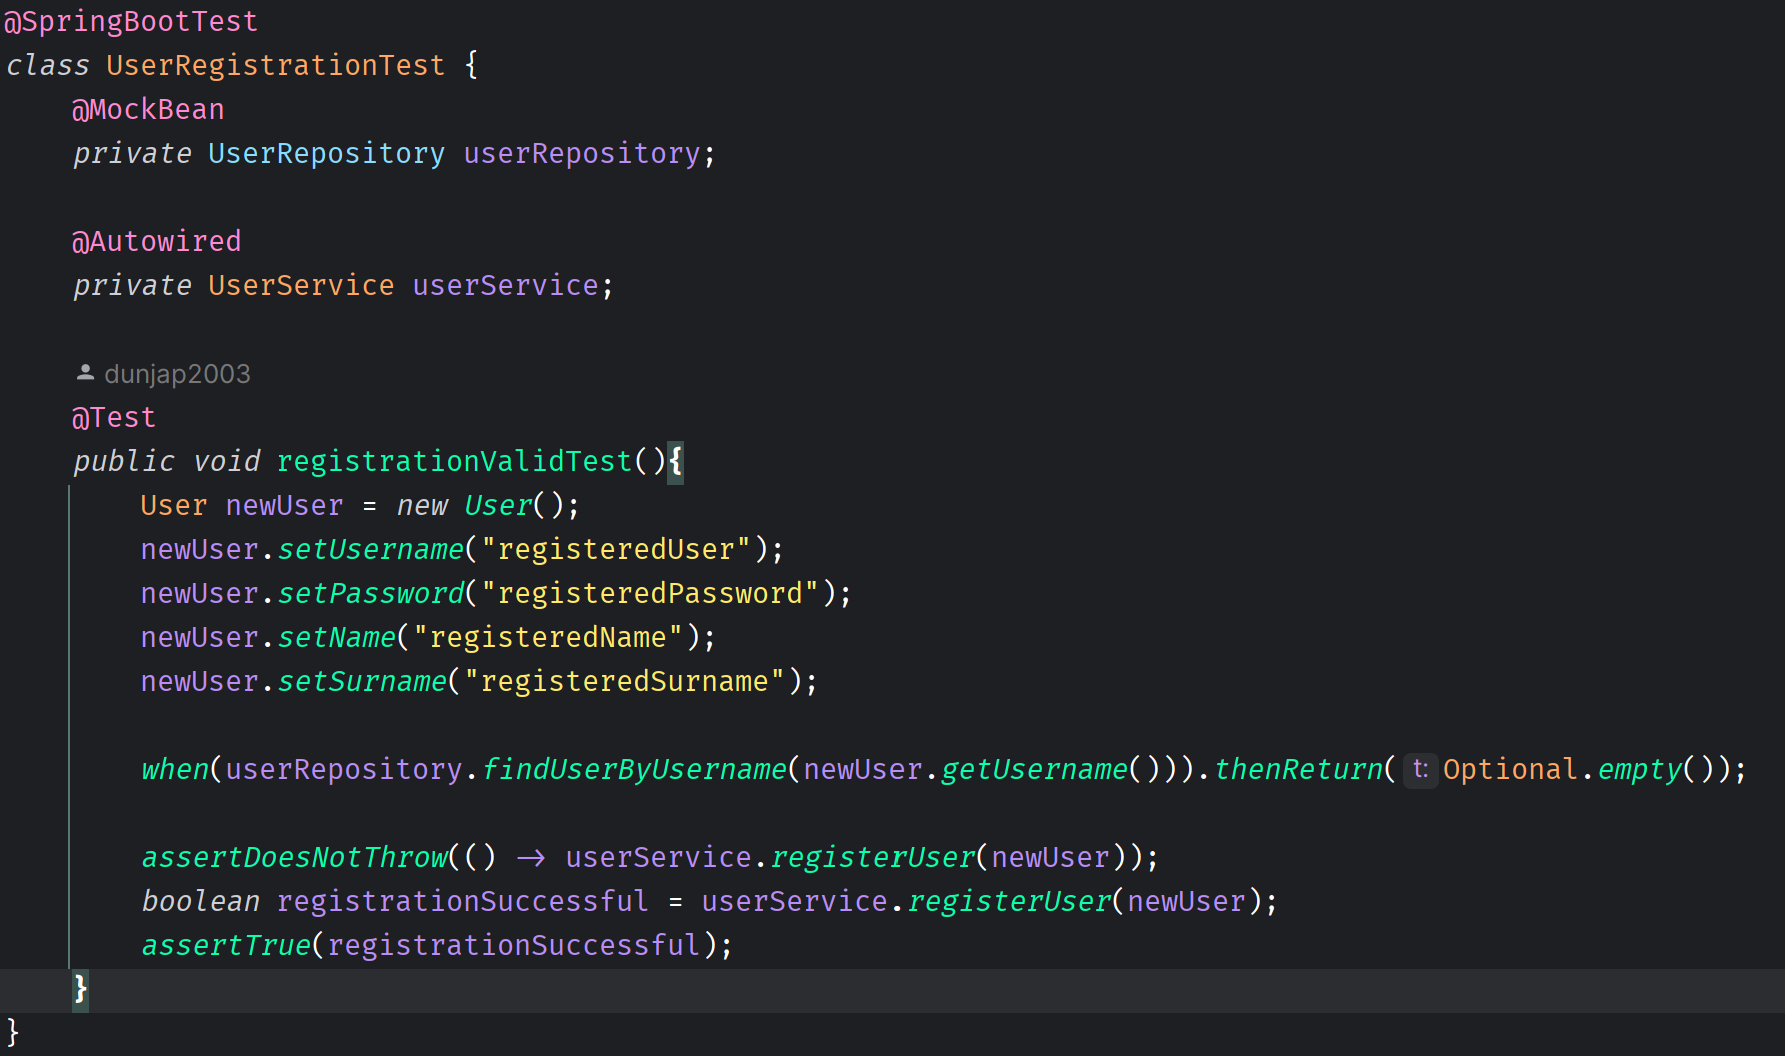
\includegraphics[scale=0.4]{slike/userRegistrationTest.PNG} %veličina slike u odnosu na originalnu datoteku i pozicija slike
			\centering
			\caption{Test uspješne registracije korisnika}
			\label{Test uspješne registracije korisnika}
		\end{figure}
		
					\begin{figure}[H]
			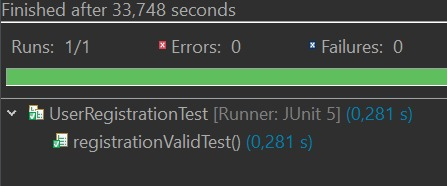
\includegraphics[scale=0.4]{slike/JUnit_register.JPG} %veličina slike u odnosu na originalnu datoteku i pozicija slike
			\centering
			\caption{Potvrda uspješnog izvođenja testa registracije}
			\label{Potvrda uspješnog izvođenja testa registracije}
		\end{figure}
		
		
\textbf{Test 2: Uspješna prijava korisnika} \\
Provedeno je testiranje ispravne prijave korisnika koji je registriran i prisutan u bazi. Prijava je uspješna ako metoda "loginUser" klase UserService ne vraća null vrijednost i ako su svi atributi prethodno stvorenog objekta korisnika i atributi korisnika koji je spremljen u oponašan repozitorij korisnika jednaki. Na slikama ispod prikazani su test uspješne prijave korisnika i metoda "loginUser" klase UserService.

				\begin{figure}[H]
			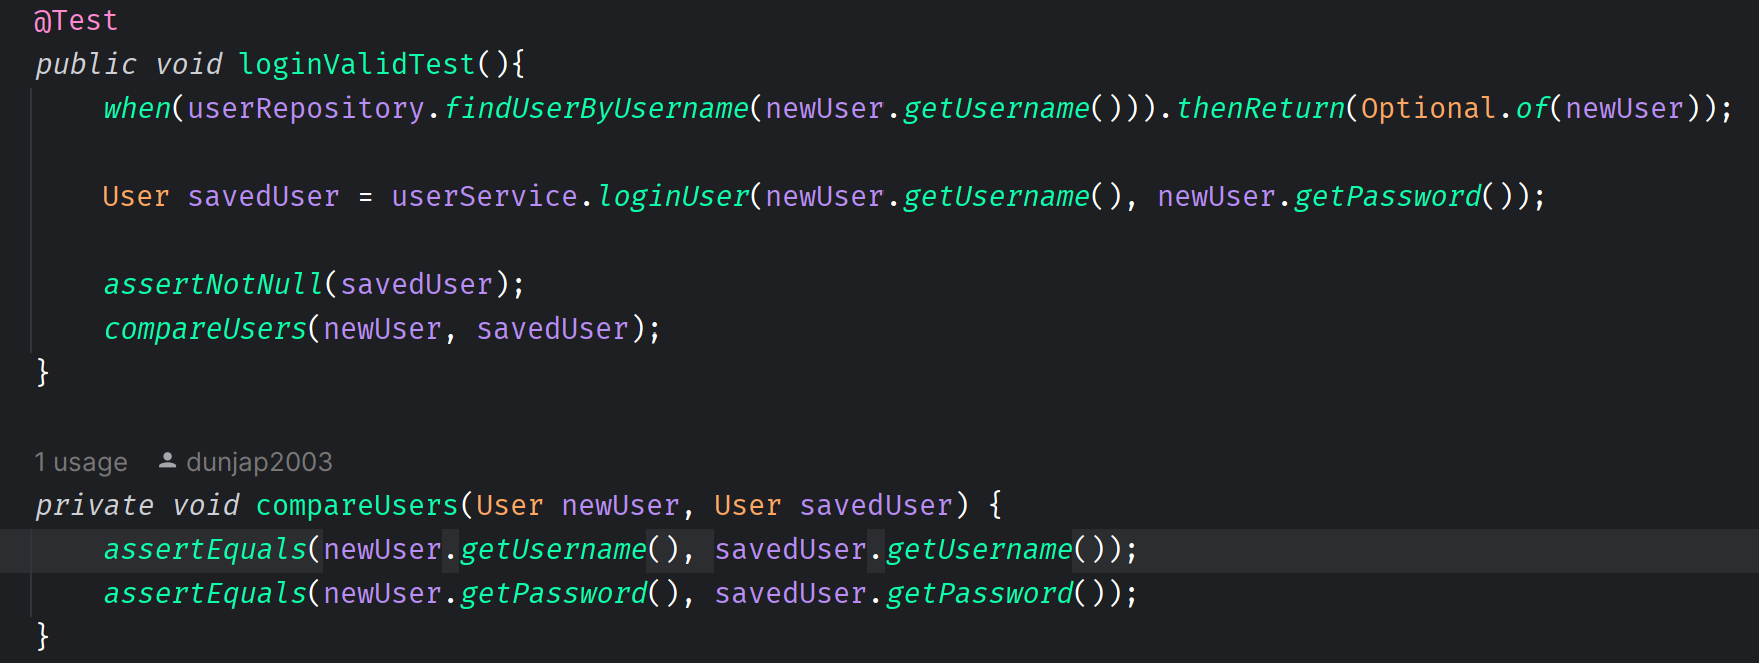
\includegraphics[scale=0.4]{slike/loginValidTest.PNG} %veličina slike u odnosu na originalnu datoteku i pozicija slike
			\centering
			\caption{Test uspješne prijave korisnika}
			\label{Test uspješne prijave korisnika}
		\end{figure}
		
						\begin{figure}[H]
			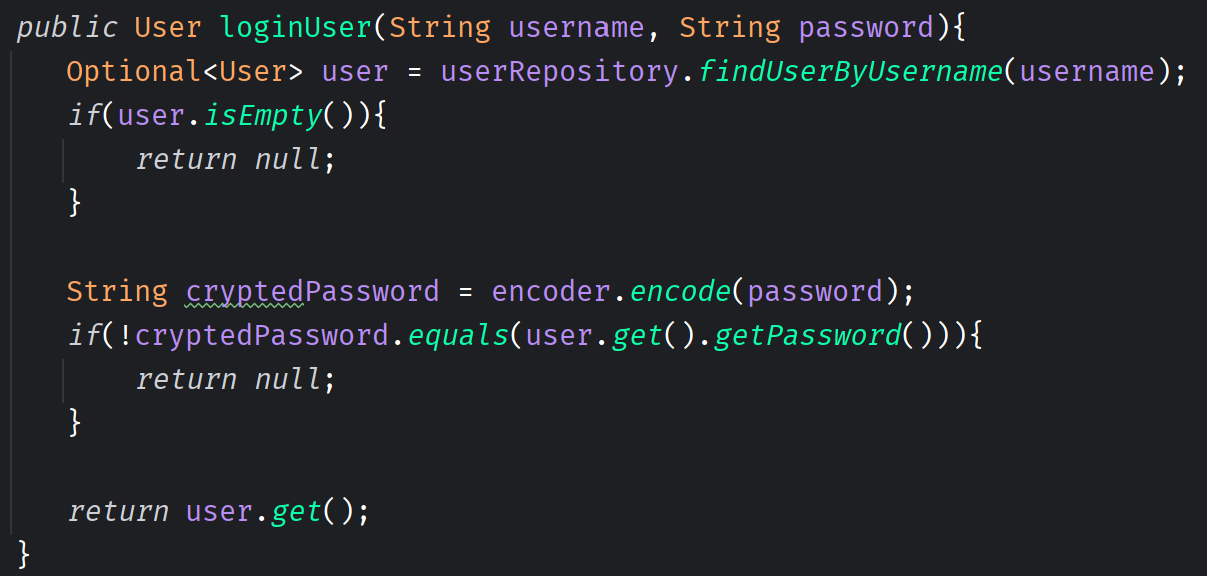
\includegraphics[scale=0.4]{slike/loginUser.PNG} %veličina slike u odnosu na originalnu datoteku i pozicija slike
			\centering
			\caption{Metoda "loginUser" klase UserService}
			\label{Metoda "loginUser" klase UserService}
		\end{figure}
		
\textbf{Test 3: Neuspješna prijava korisnika (nepostojeće korisničko ime)} \\
Provedeno je testiranje neuspješne prijave korisnika zbog unosa neispravnog korisničkog imena, tj. korisničkog imena koje se ne nalazi u oponašanom repozitoriju korisnika koji je simuliran u sklopu testiranja. Neuspješna prijava korisnika manifestira se kroz dohvaćenu null vrijednost prilikom dohvaćanja traženog korisnika iz oponašanog repozitorija korisnika. Na slici ispod prikazan je test neuspješne prijave korisnika zbog nepostojećeg korisničkog imena. Metoda "loginUser" klase UserService prikazana je u slici iznad.

				\begin{figure}[H]
			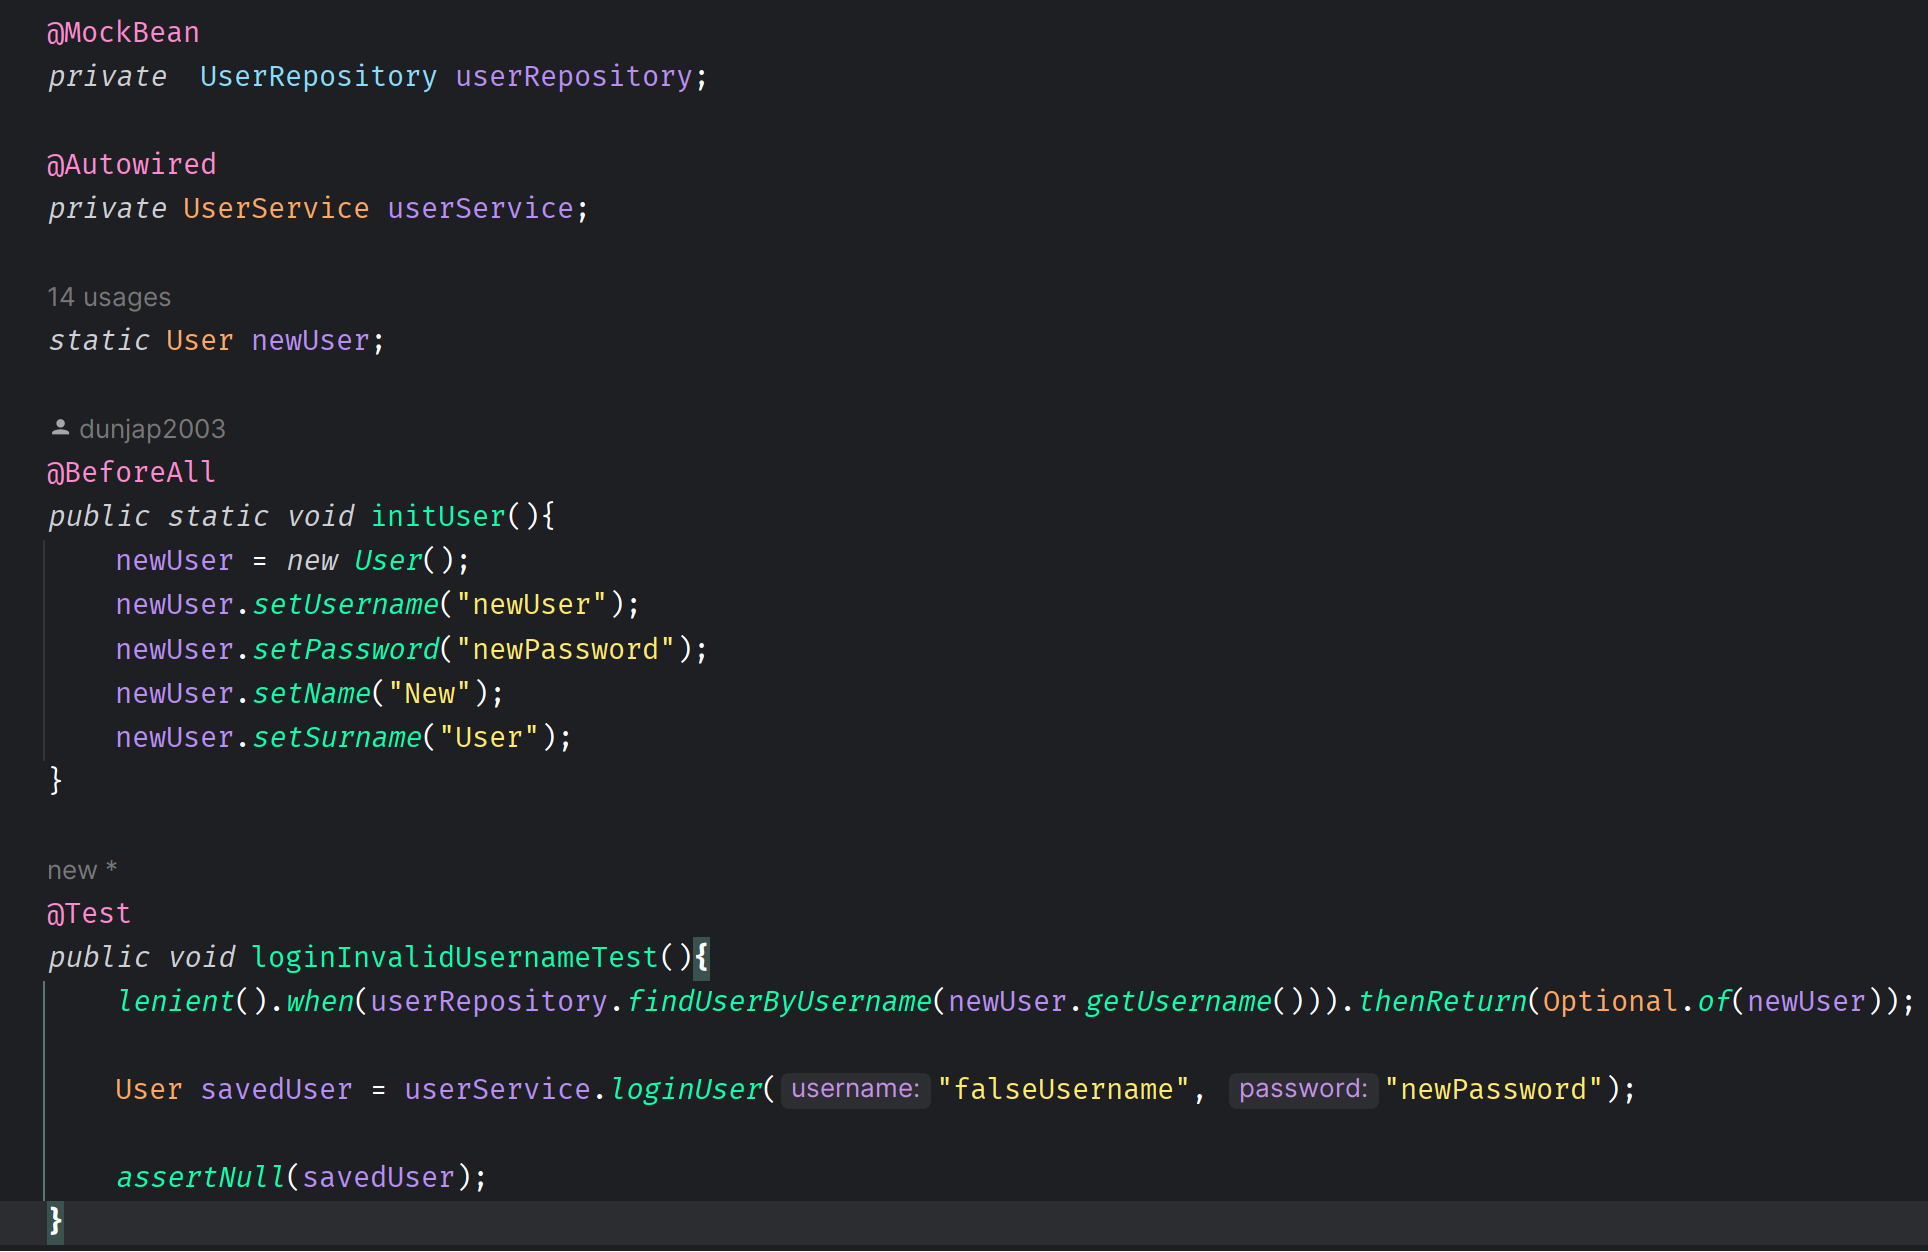
\includegraphics[scale=0.4]{slike/loginInvalidUsernameTest.PNG} %veličina slike u odnosu na originalnu datoteku i pozicija slike
			\centering
			\caption{Test neuspješne prijave korisnika zbog nepostojećeg korisničkog imena}
			\label{Test neuspješne prijave korisnika zbog nepostojećeg korisničkog imena}
		\end{figure}
		
\textbf{Test 4: Neuspješna prijava korisnika (pogrešna lozinka)} \\
Provedeno je testiranje neuspješne prijave korisnika zbog unosa ispravnog korisničkog imena, ali neispravne lozinke koja bi omogućila pristup profilu s tim korisničkim imenom. Neuspješna prijava korisnika zbog neispravne lozinke manifestira se kroz dohvaćenu null vrijednost prilikom usporedbi lozinki spremljenog korisnika s tim korisničkim imenom i upisane lozinke za to korisničko ime. Na slici ispod prikazan je test neuspješne prijave korisnika zbog upisane neispravne lozinke. Metoda "loginUser" klase UserService prikazana je u slici iznad.

				\begin{figure}[H]
			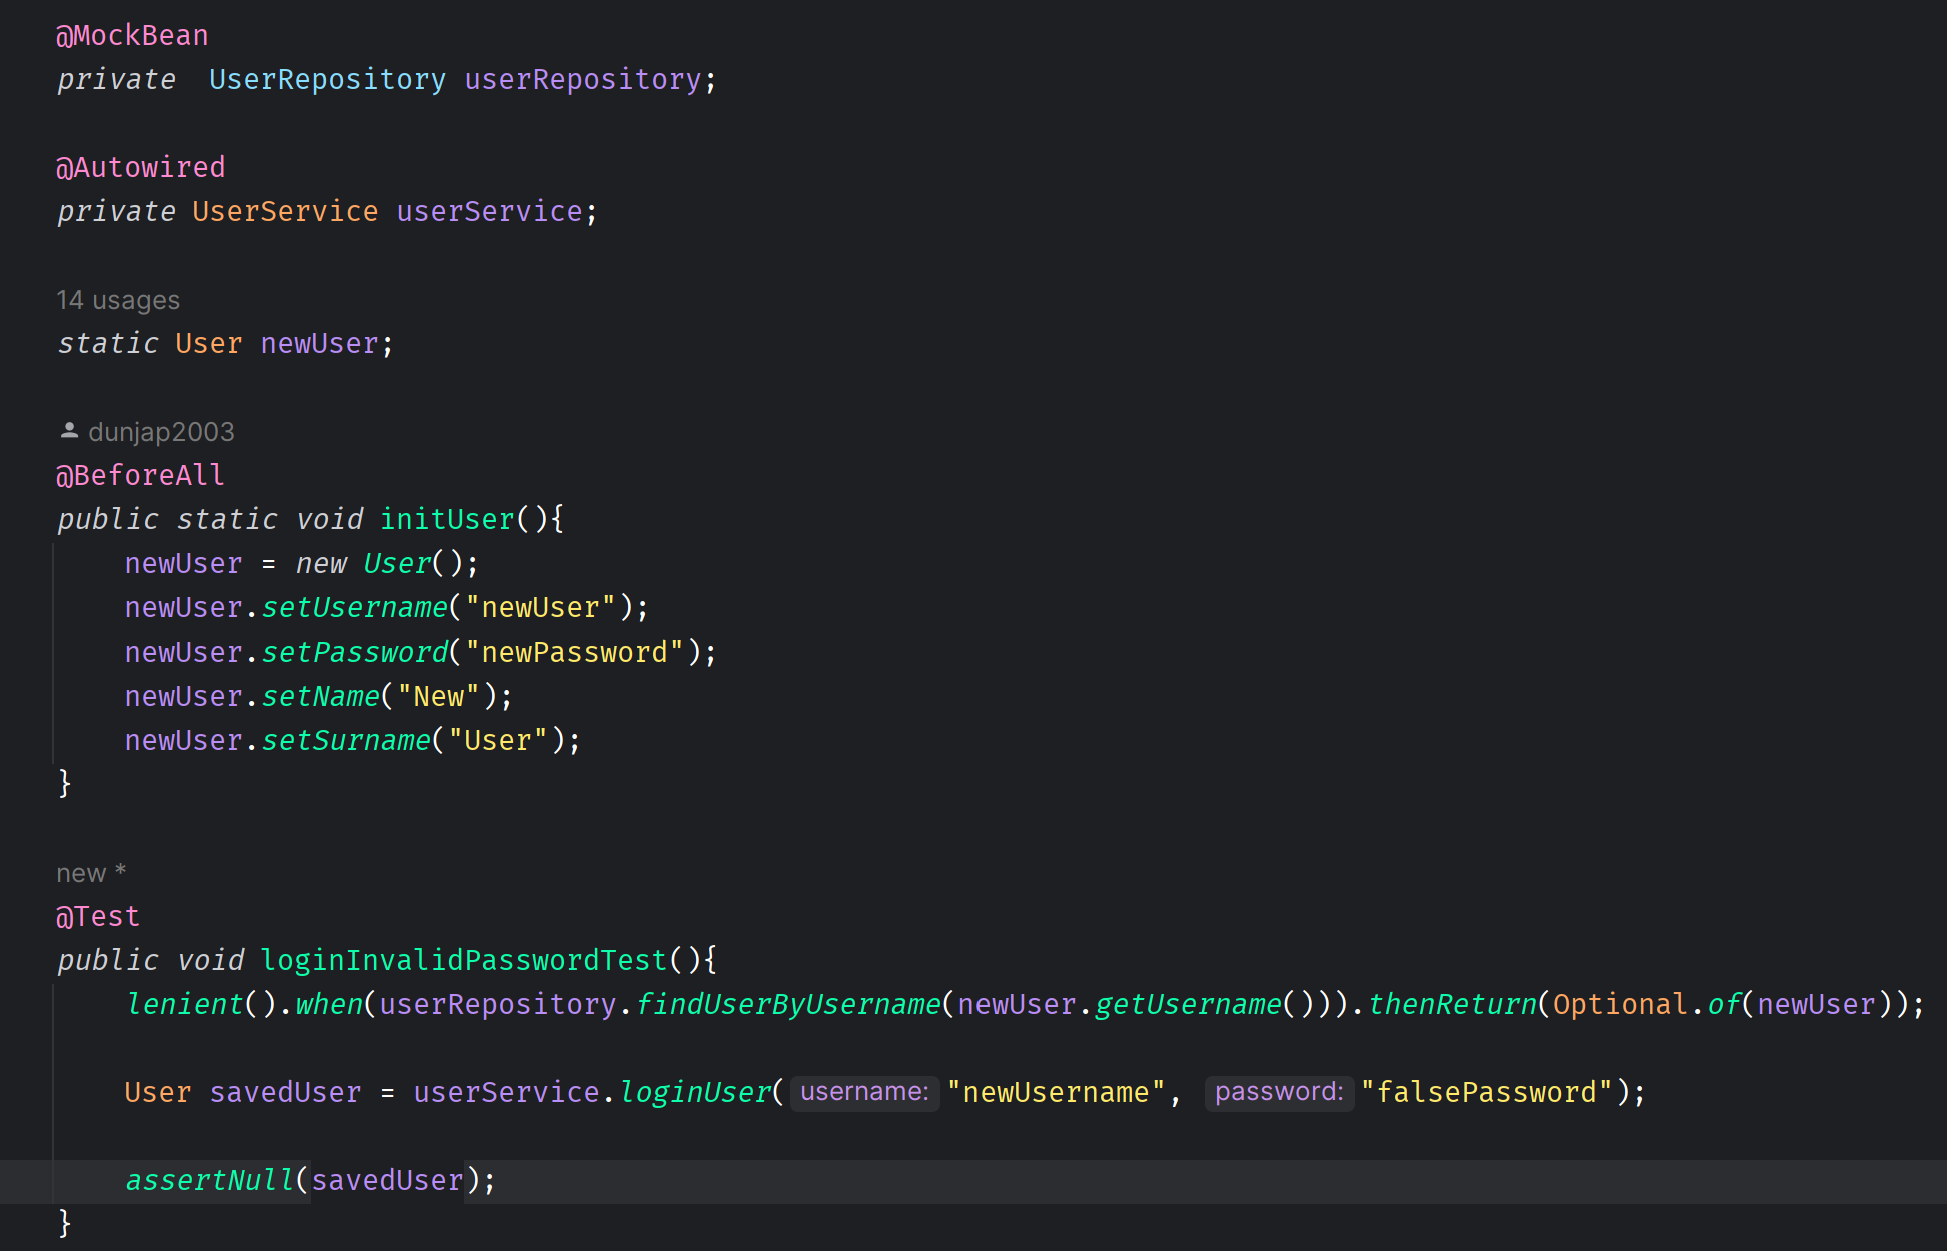
\includegraphics[scale=0.4]{slike/loginInvalidPasswordTest.PNG} %veličina slike u odnosu na originalnu datoteku i pozicija slike
			\centering
			\caption{Test neuspješne prijave korisnika zbog unosa neispravne lozinke}
			\label{Test neuspješne prijave korisnika zbog unosa neispravne lozinke}
		\end{figure}
		
		Na slici ispod prikazane su potvrde uspješnog izvođenja testova vezanih uz login.
		
			\begin{figure}[H]
			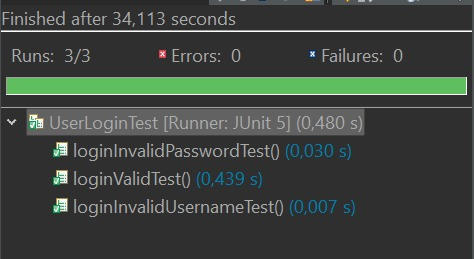
\includegraphics[scale=0.4]{slike/JUnit_login.JPG} %veličina slike u odnosu na originalnu datoteku i pozicija slike
			\centering
			\caption{Potvrda uspješnog izvođenja testova vezanih uz login}
			\label{Potvrda uspješnog izvođenja testova vezanih uz login}
		\end{figure}
			
\textbf{Test 5: Uspješno dohvaćanje podataka o korisniku iz baze podataka} \\

Provedeno je testiranje uspješnog dohvaćanja podataka o korisniku iz baze podataka. Dohvaćanje podataka o korisniku iz baze podataka je uspješno ako metoda "loadUserByUsername" klase UserService vrati objekt korisnika koji je pronađen putem korisničkog imena i ako su atributi korisnika dohvaćenog iz oponašanog repozitorija korisnika i atributi onog korisnika koji je inicijalno spremljen u oponašani repozitorij jednaki. Na slikama ispod prikazani su test uspješnog dohvaćanja podataka o korisniku iz baze podataka te metoda "loadUserByUsername" klase UserService, kao i potvrda uspješno izvedenog testa o dohvaćanju podataka o korisniku iz baze podataka.

				\begin{figure}[H]
			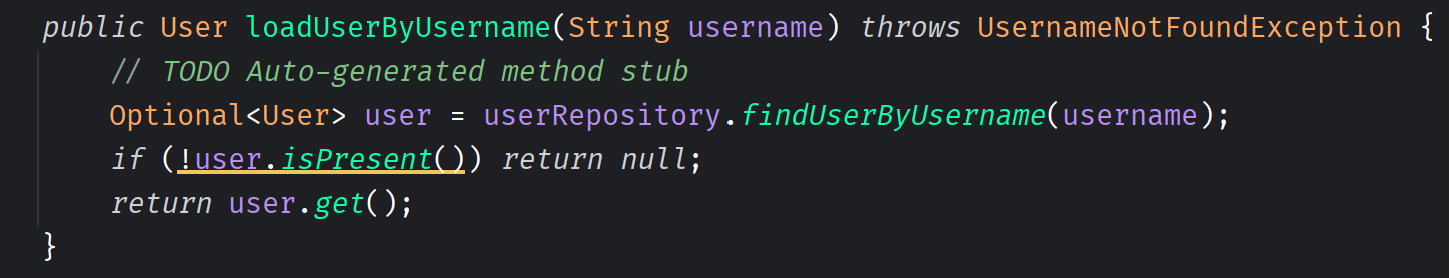
\includegraphics[scale=0.4]{slike/loadUserByUsername.PNG} %veličina slike u odnosu na originalnu datoteku i pozicija slike
			\centering
			\caption{Metoda "loadUserByUsername" klase UserService}
			\label{Metoda "loadUserByUsername" klase UserService}
		\end{figure}
		
						\begin{figure}[H]
			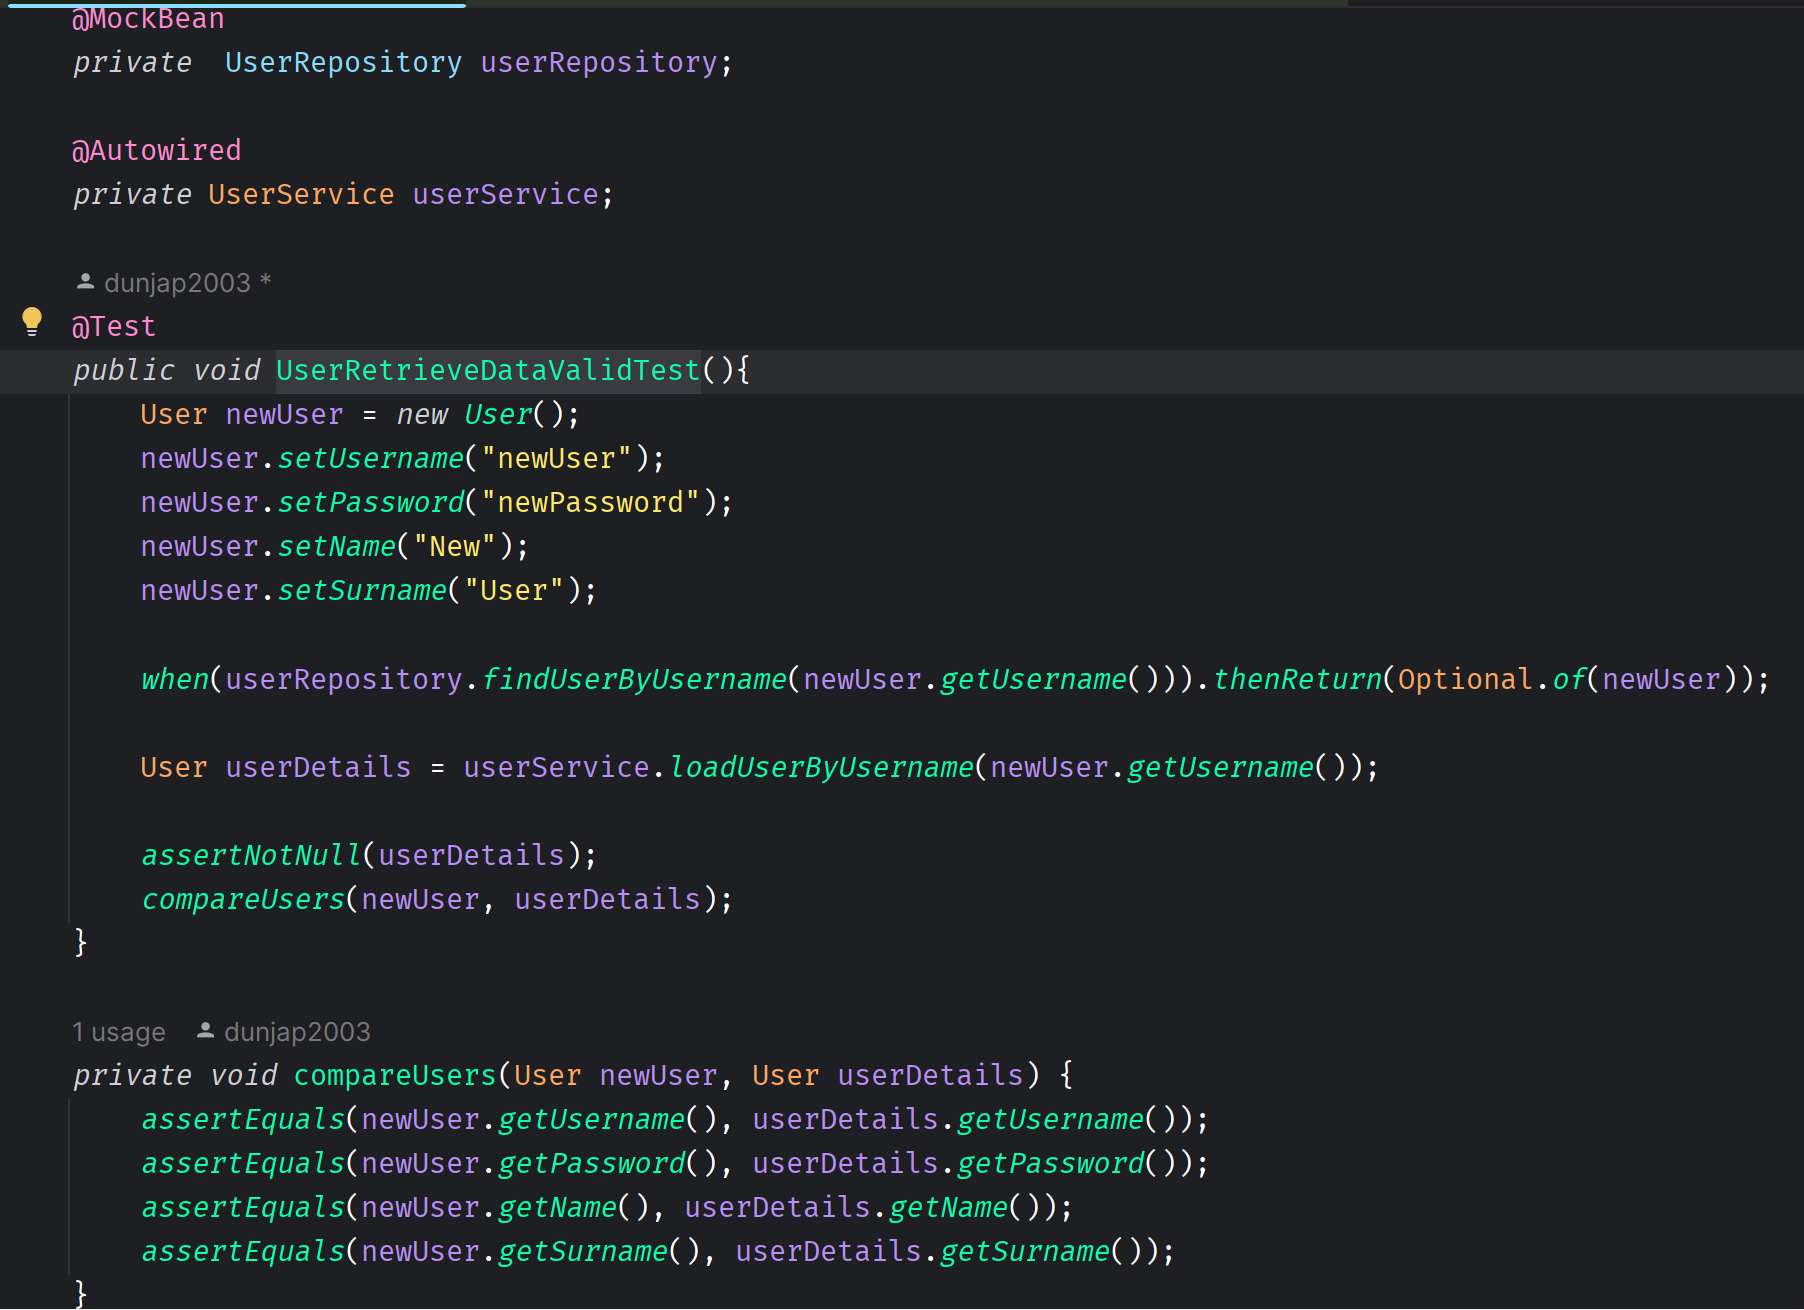
\includegraphics[scale=0.4]{slike/userRetrieveDataValidTest.PNG} %veličina slike u odnosu na originalnu datoteku i pozicija slike
			\centering
			\caption{Test uspješnog dohvaćanja podataka o korisniku na temelju korisničkog imena iz baze podataka}
			\label{Test uspješnog dohvaćanja podataka o korisniku na temelju korisničkog imena iz baze podataka}
		\end{figure}
		
			\begin{figure}[H]
			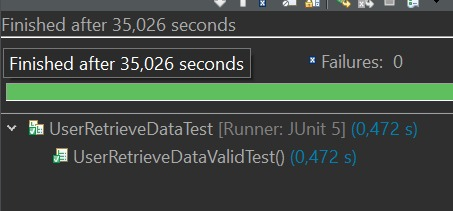
\includegraphics[scale=0.4]{slike/JUnit_retrieve.JPG} %veličina slike u odnosu na originalnu datoteku i pozicija slike
			\centering
			\caption{Potvrda uspješnog izvođenja testa dohvaćanja podataka o korisniku}
			\label{Potvrda uspješnog izvođenja testa dohvaćanja podataka o korisniku}
		\end{figure}
		
\textbf{Test 6: Uspješna promjena podataka korisnika} \\
Provedeno je testiranje uspješne promjene podataka korisnika koji se nalazi u bazi. Promjena podataka je uspješna ako metoda "changeInfo" klase UserServive uspješno osvježi željene podatke u bazi podataka (podaci o korisniku u oponašanom repozitoriju korisnika odgovaraju podacima koji su zadani kao zamjena originalnima). Na slikama ispod prikazani su test uspješne promjene podataka korisnika te metoda "changeInfo" klase UserService, kao i potvrda uspješnog izvođenja testa o promjeni podataka korisnika.

				\begin{figure}[H]
			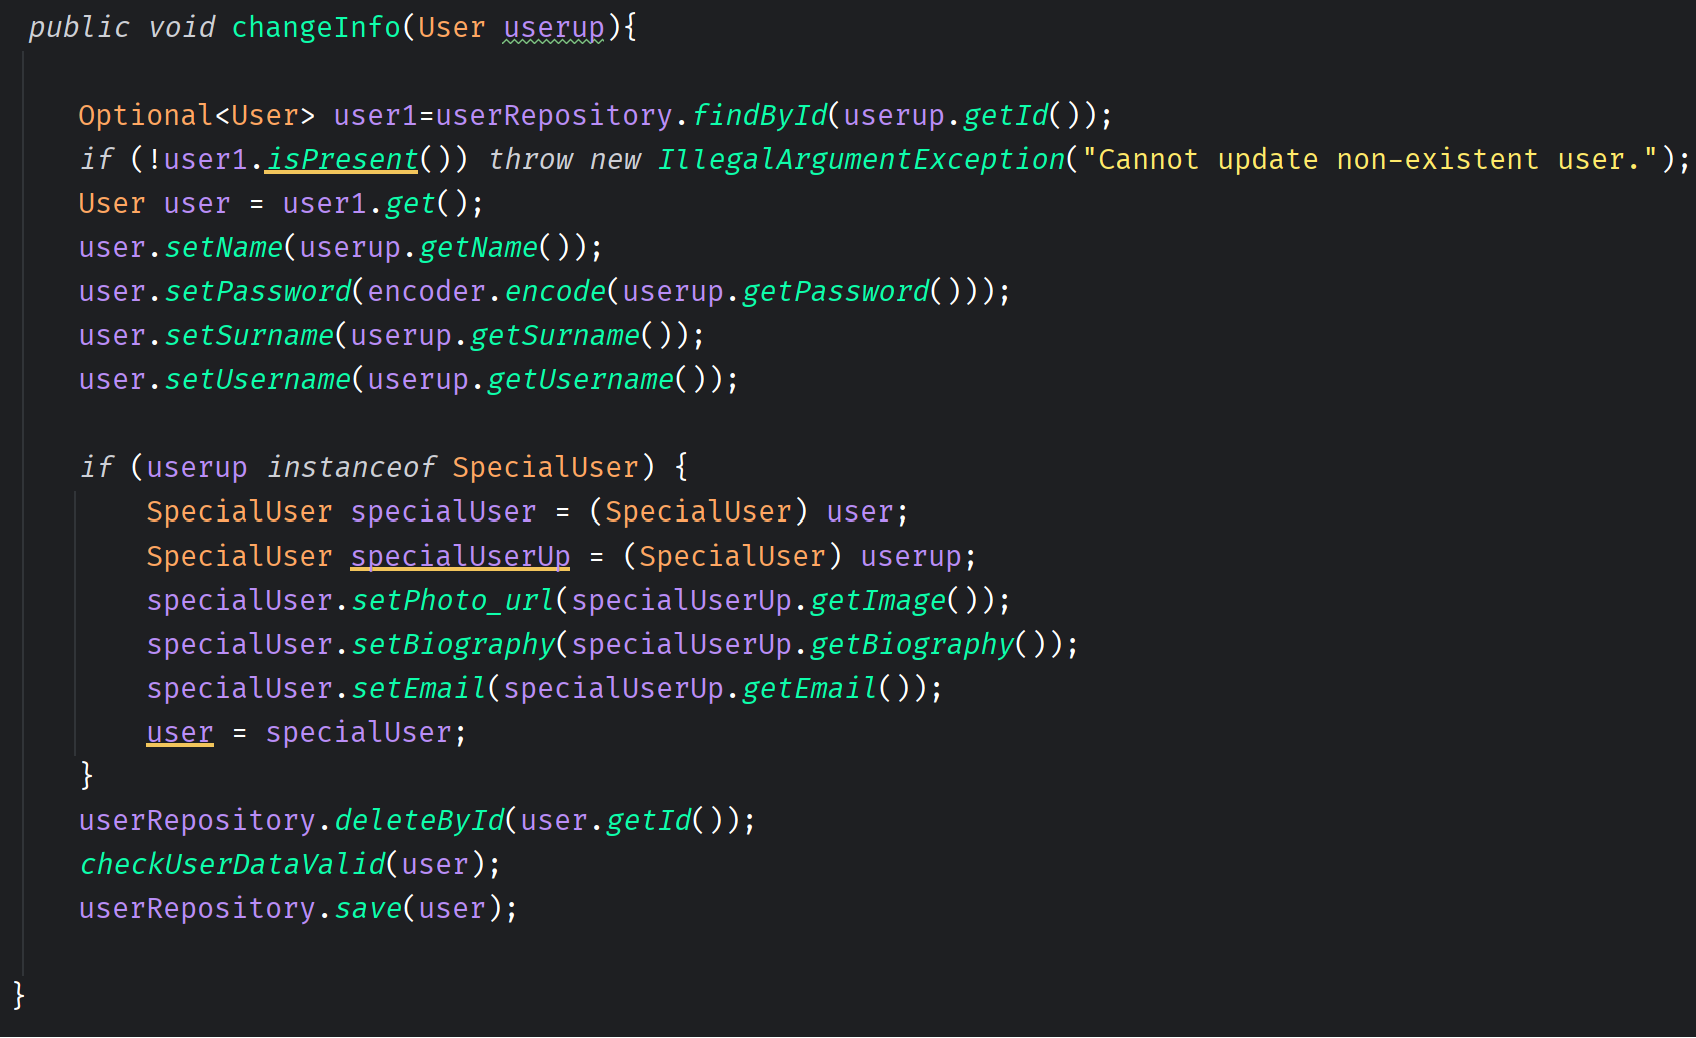
\includegraphics[scale=0.4]{slike/changeInfo.PNG} %veličina slike u odnosu na originalnu datoteku i pozicija slike
			\centering
			\caption{Metoda "changeInfo" klase UserService}
			\label{Metoda "changeInfo" klase UserService}
		\end{figure}
		
			\begin{figure}[H]
			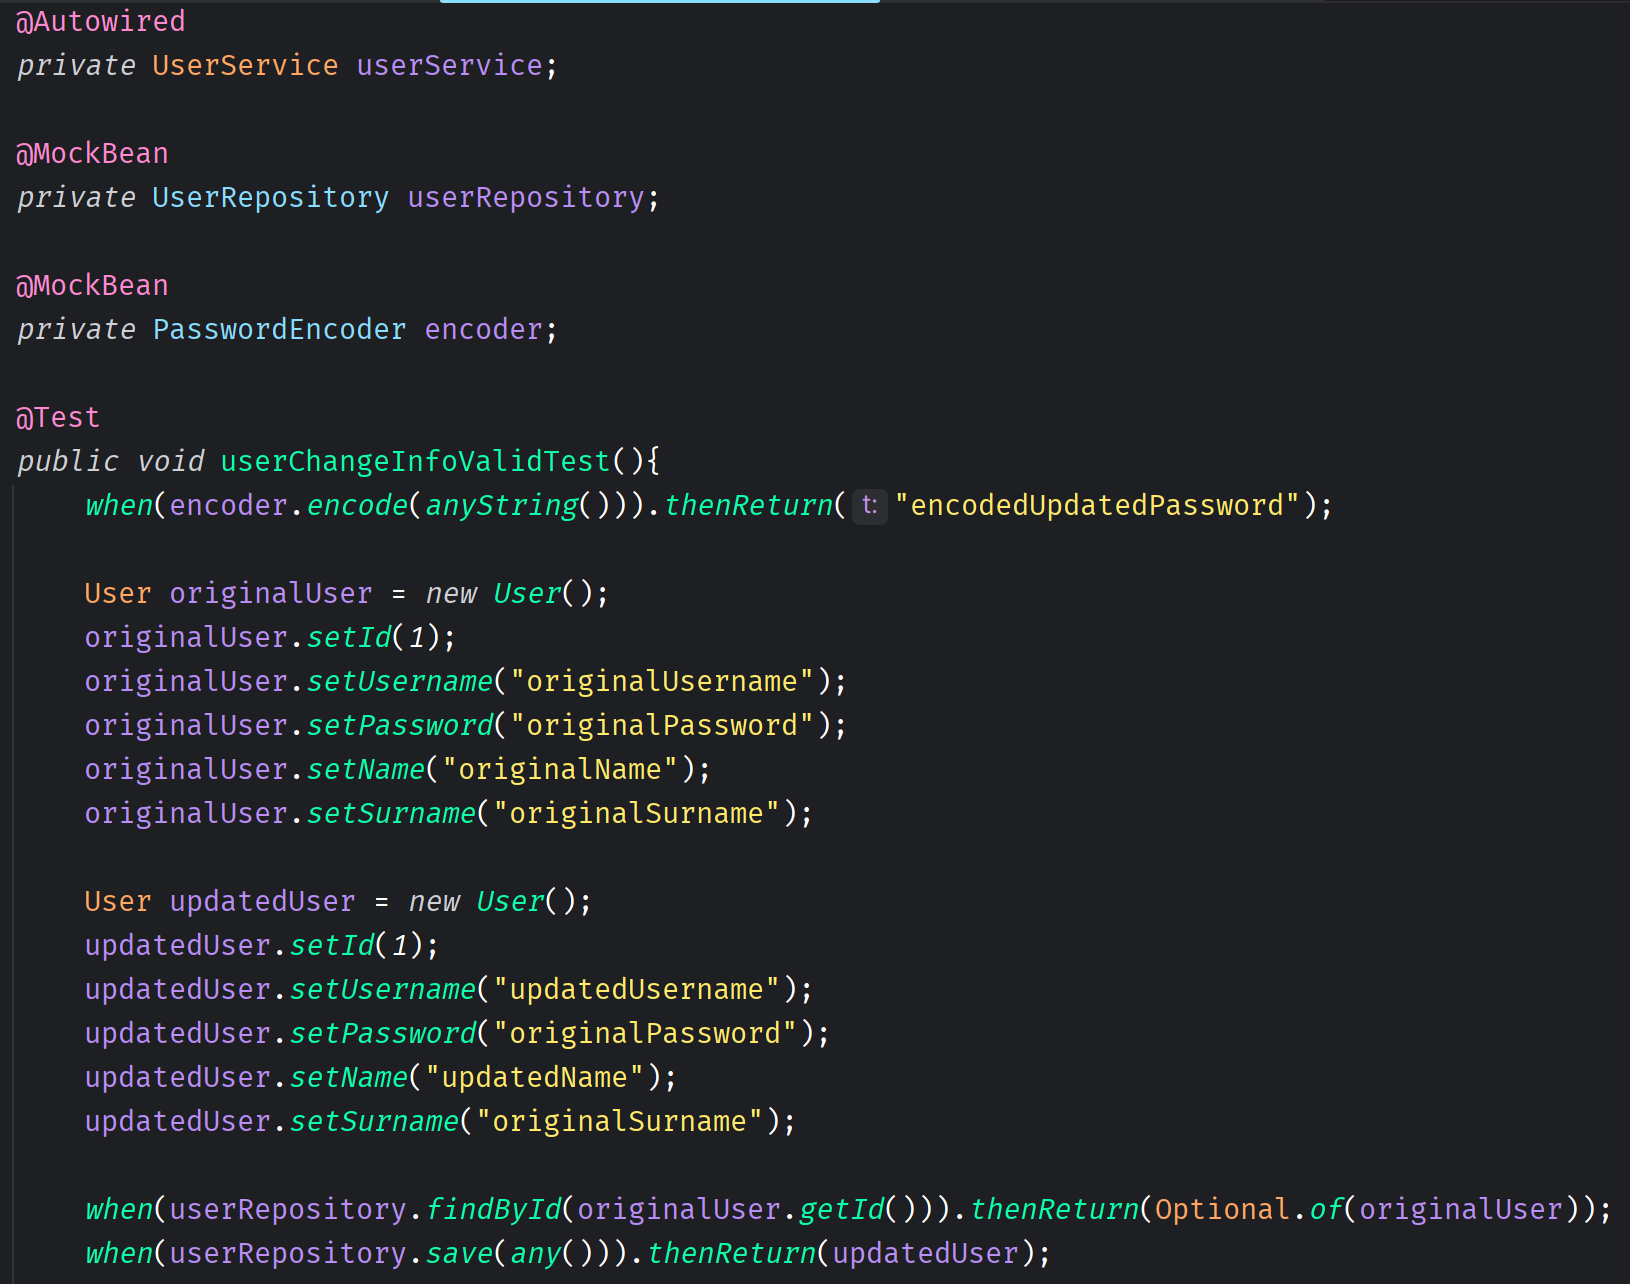
\includegraphics[scale=0.4]{slike/userChangeInfoValidTest1.PNG} %veličina slike u odnosu na originalnu datoteku i pozicija slike
			\centering
			\caption{Test uspješne promjene podataka korisnika u bazi, 1. dio}
			\label{Test uspješne promjene podataka korisnika u bazi, 1. dio}
		\end{figure}
		
								\begin{figure}[H]
			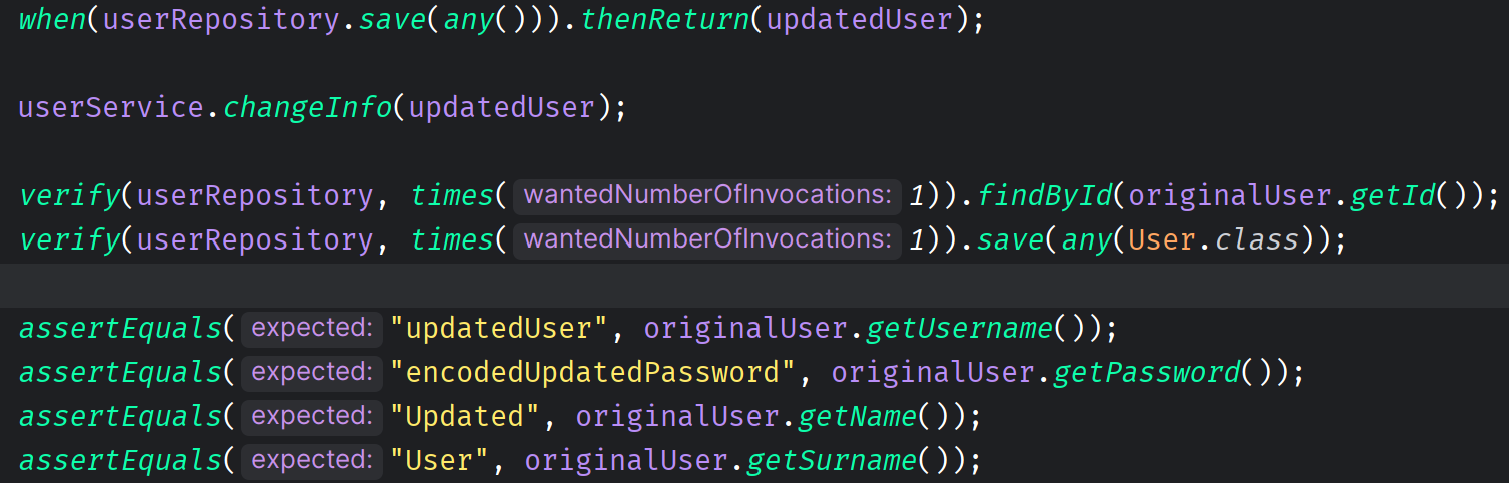
\includegraphics[scale=0.4]{slike/userChangeInfoValidTest2.PNG} %veličina slike u odnosu na originalnu datoteku i pozicija slike
			\centering
			\caption{Test uspješne promjene podataka korisnika u bazi, 2. dio}
			\label{Test uspješne promjene podataka korisnika u bazi, 2. dio}
		\end{figure}
		
		\begin{figure}[H]
			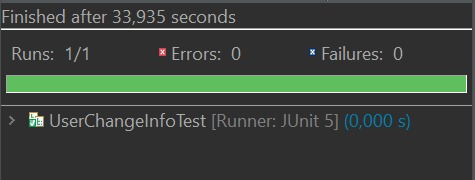
\includegraphics[scale=0.4]{slike/JUnit_change.JPG} %veličina slike u odnosu na originalnu datoteku i pozicija slike
			\centering
			\caption{Potvrda uspješnog izvođenja testova vezanih uz promjenu podataka korisnika}
			\label{Potvrda uspješnog izvođenja testova vezanih uz promjenu podataka korisnika}
		\end{figure}
			
		
	
		
		\textbf{Test 7: Uspješno dohvaćanje recepata po korisničkom imenu autora recepata}
		
		Provedeno je testiranje uspješnog dohvaćanja recepata po korisničkom imenu autora recepata. Dohvaćanje recepata je uspješno ako dohvaćeni set recepata kojima je autor stvoreni korisnik nije null vrijednost te ako su očekivani set recepata i dohvaćeni set recepata jednaki. Na slikama ispod prikazani su test uspješnog dohvaćanja recepata po korisničkom imenu autora recepata te metoda "getRecipesByUsername" klase RecipeService.
		
		DODAJ TE DVIJE SLIKE
		
		
		\textbf{Test 8: Uspješno dohvaćanje recepata po kategoriji recepta}
		
		Provedeno je testiranje uspješnog dohvaćanja recepata po kategoriji recepta. Dohvaćanje recepata je uspješno ako dohvaćeni set recepata iz oponašanog repozitorija recepata s određenom kategorijom nije null vrijednost te ako su očekivani set recepata i dohvaćeni set recepata jednaki. Na slikama ispod prikazani su test uspješnog dohvaćanja recepata po kategoriji te metoda "getRecipesByCategory" klase RecipeService.
		
		DODAJ TE DVIJE SLIKE

		
		

















			
			
			
			\subsection{Ispitivanje sustava}
			
			 \textit{Potrebno je provesti i opisati ispitivanje sustava koristeći radni okvir Selenium\footnote{\url{https://www.seleniumhq.org/}}. Razraditi \textbf{minimalno 4 ispitna slučaja} u kojima će se ispitati redovni slučajevi, rubni uvjeti te poziv funkcionalnosti koja nije implementirana/izaziva pogrešku kako bi se vidjelo na koji način sustav reagira kada nešto nije u potpunosti ostvareno. Ispitni slučaj se treba sastojati od ulaza (npr. korisničko ime i lozinka), očekivanog izlaza ili rezultata, koraka ispitivanja i dobivenog izlaza ili rezultata.\\ }
			 
			 \textit{Izradu ispitnih slučajeva pomoću radnog okvira Selenium moguće je provesti pomoću jednog od sljedeća dva alata:}
			 \begin{itemize}
			 	\item \textit{dodatak za preglednik \textbf{Selenium IDE} - snimanje korisnikovih akcija radi automatskog ponavljanja ispita	}
			 	\item \textit{\textbf{Selenium WebDriver} - podrška za pisanje ispita u jezicima Java, C\#, PHP koristeći posebno programsko sučelje.}
			 \end{itemize}
		 	\textit{Detalji o korištenju alata Selenium bit će prikazani na posebnom predavanju tijekom semestra.}
			
			\eject 
		
		
		\section{Dijagram razmještaja}
			
		
		Na slici 5.1 prikazan je dijagram razmještaja. Dijagrami razmještaja prikazuju fizičku arhitekturu programskog sustava, prikazujući razmještaj programskih artefakata na sklopovskim čvorovima ili virtualnim okruženjima. Glavna svrha dijagrama razmještaja u programskom inženjerstvu je pružiti razumijevanje arhitekture razmještaja sustava.
		
		Naš dijagram razmještaja sastoji se od dvije glavne komponente: računalo korisnika i poslužiteljsko računalo. Na računalu korisnika, on putem web preglednika pristupa aplikaciji KuhajIT. Komunikacija između računala korisnika i poslužiteljskog računala uspostavlja se i odvija pomoću protokola HTTP. Unutar poslužiteljskog računala razlikujemo dvije podkomponente: web poslužitelj i poslužitelj baze podataka.
		
					\begin{figure}[H]
			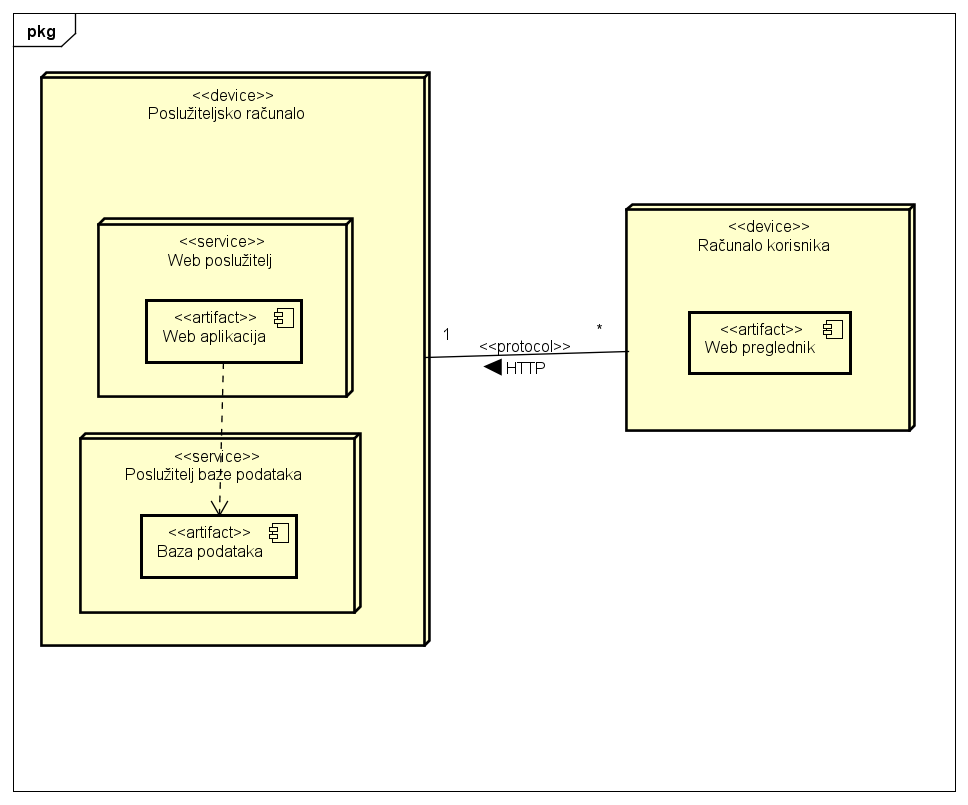
\includegraphics[scale=0.4]{dijagrami/UML_dijagram_razmjestaja.PNG} %veličina slike u odnosu na originalnu datoteku i pozicija slike
			\centering
			\caption{Dijagram razmještaja}
			\label{Dijagram razmještaja}
		\end{figure}
		
		

			\eject 
		
		\section{Upute za puštanje u pogon}
		Naša KuhajIT web-aplikacija, razvijena u okviru ovog projekta, puštena je u pogon putem web platforme  \textcolor{blue}{\underline{\href{https://render.com/}{\textcolor{blue}{Render}}}}\footnote{\url{https://render.com/}}. Render je platforma koja pruža usluge za deploy, hosting i skaliranje web aplikacija, servisa i web stranica. Ističe se jednostavnošću upotrebe, brzim implementacijama i podrškom za različite jezike i okvire, i upravo smo ju zbog tog razloga i odabrali za tzv. deploy. Na Render-u je postavljen Spring Boot poslužitelj, kojega smo spremili u Docker kontejner, a koji odgovara na upite korisnika, statička stranica, koja služi za prikaz React web aplikacije te PostgreSQL baza podataka. Ispod su priložene dvije slike komponenata postavljenih na Render.
		
		
			\begin{figure}[H]
			
\includegraphics[scale=0.3]{slike/Render_OVERVIEW.JPG} %veličina slike u odnosu na originalnu datoteku i pozicija slike
			\centering
			\caption{Pregled prenesenih komponenti, frontend i backend}
			\label{Pregled prenesenih komponenti, frontend i backend}
		\end{figure}
		
					\begin{figure}[H]
			
\includegraphics[scale=0.3]{slike/Render_OVERVIEW_DATABASE.JPG} %veličina slike u odnosu na originalnu datoteku i pozicija slike
			\centering
			\caption{Pregled prenesenih komponenti, baza podataka}
			\label{Pregled prenesenih komponenti, baza podataka}
		\end{figure}
		
		
		
		\textbf{Postavljanje Spring Boot poslužitelja} \\
		Dio razloga zbog kojeg smo odabrali baš Render za deploy je jednostavnost postavljanja komponenti na njega. Tako je bilo i s postavljanjem Spring Boot poslužitelja koji komunicira sa React aplikacijom, spremljenom u \textcolor{blue}{\underline{\href{https://docker.com/}{\textcolor{blue}{Docker}}}}\footnote{\url{https://docker.com/}} "kontejner". Korištenje Docker-a nam je uvelike olakšalo cijeli proces deploy-a, jer Docker nudi izolirane okoline, zvane kontejnerima, koje sadrže sve potrebno za pokretanje aplikacije, stoga se nije potrebno oslanjati na ono što je instalirano na Render poslužitelju. Na slici ispod prikazan je kod Dockerfile-a. Dockerfile je dokument koji sadrži sve naredbe koje bi se trebale pozvati u naredbenom retku kako bi se aplikacija ispravno i cjelovito pokrenula.
		
		\begin{figure}[H]
			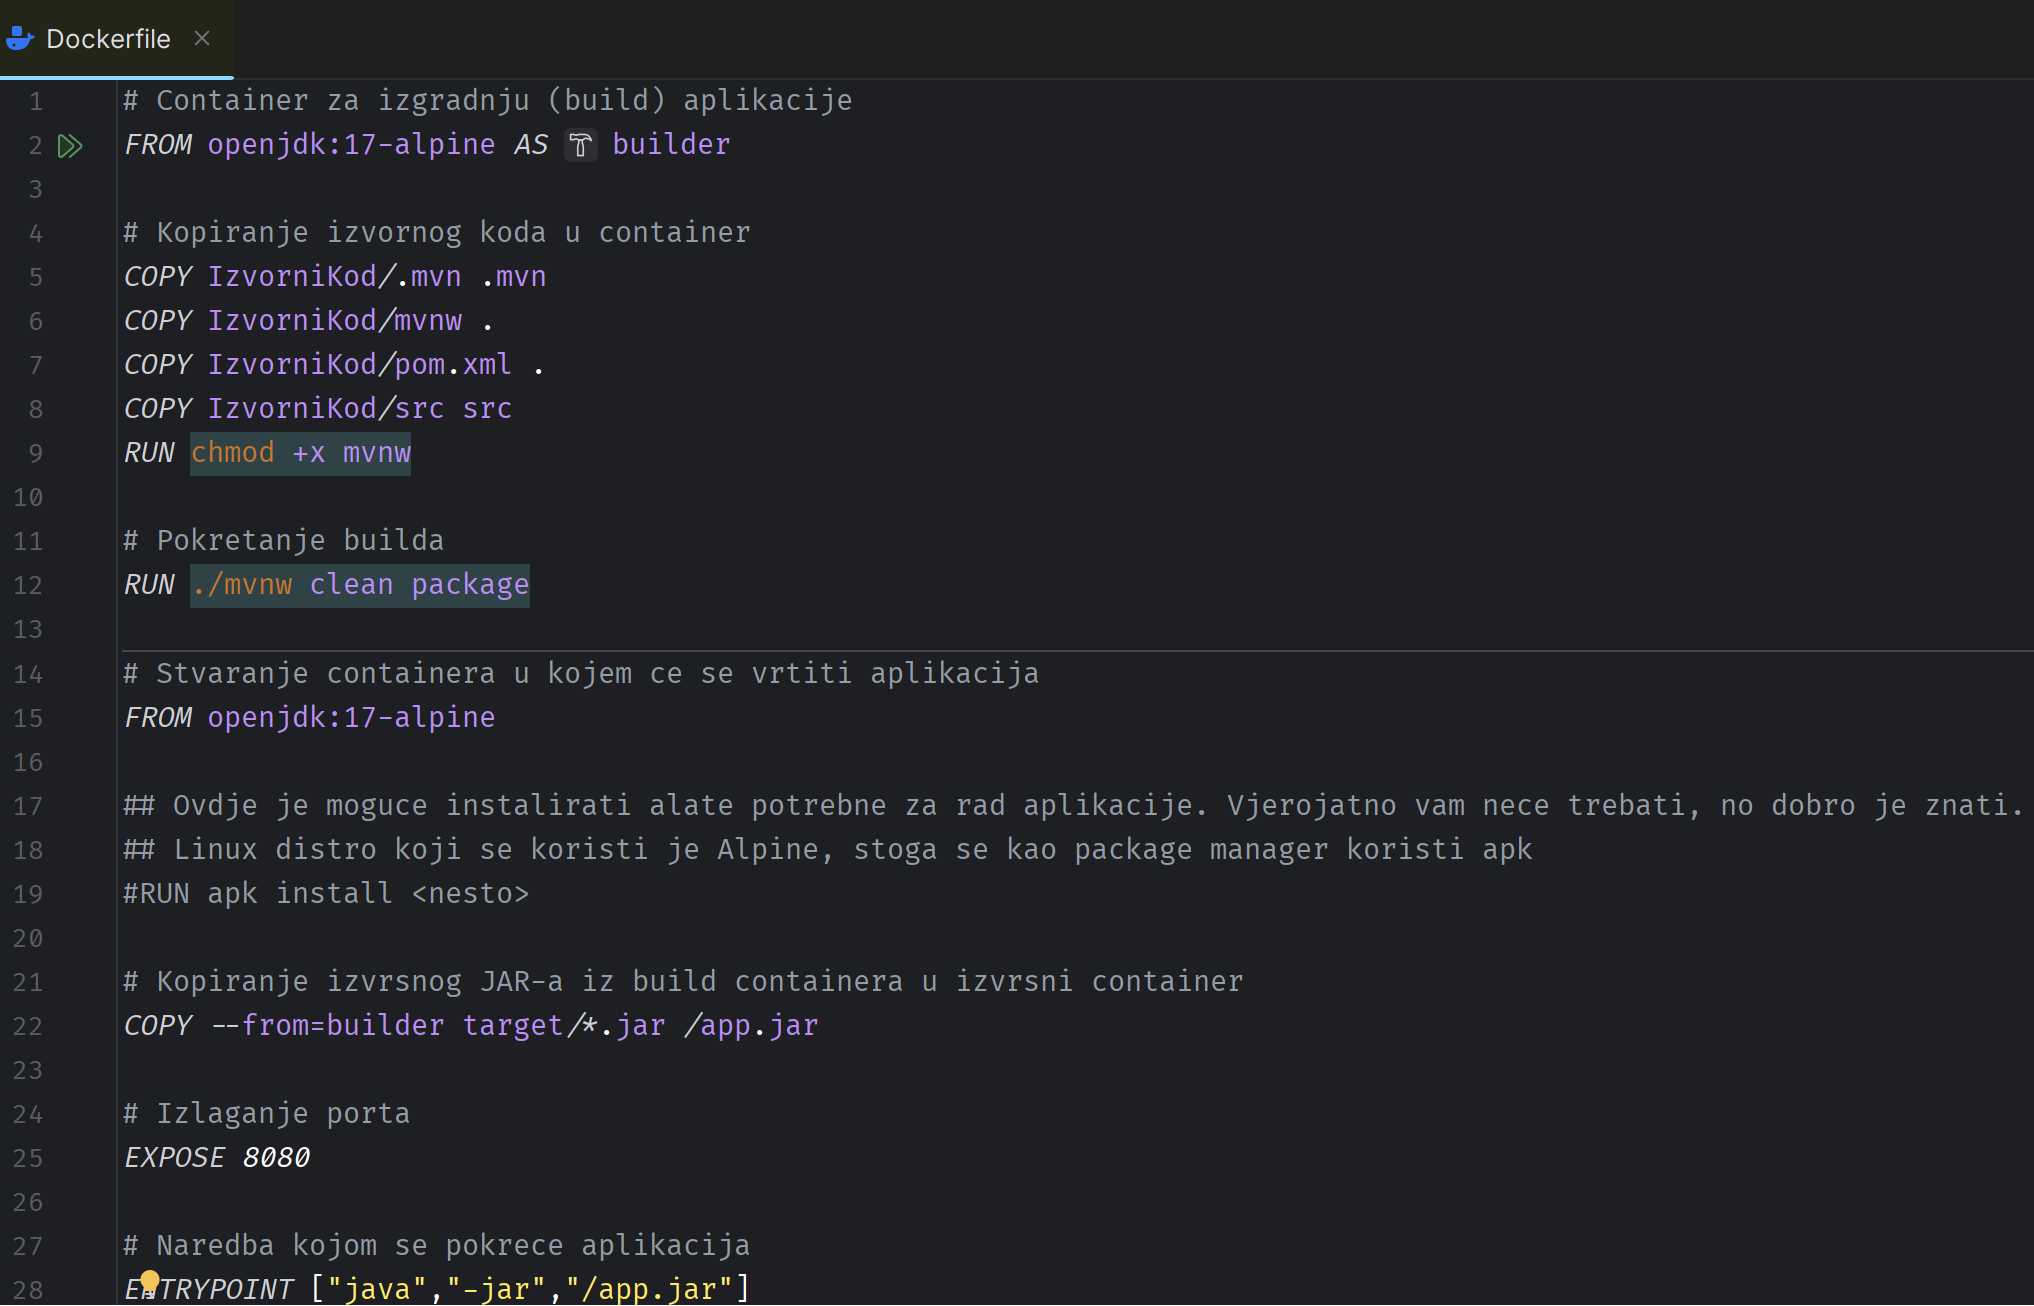
\includegraphics[scale=0.4]{slike/Dockerfile.PNG} %veličina slike u odnosu na originalnu datoteku i pozicija slike
			\centering
			\caption{Dockerfile}
			\label{Dockerfile}
		\end{figure}
		
		
Na početku, potrebno je u gornjem desnom kutu web platforme Render odabrati opciju New, kako je prikazano na slici ispod.
		
			\begin{figure}[H]
			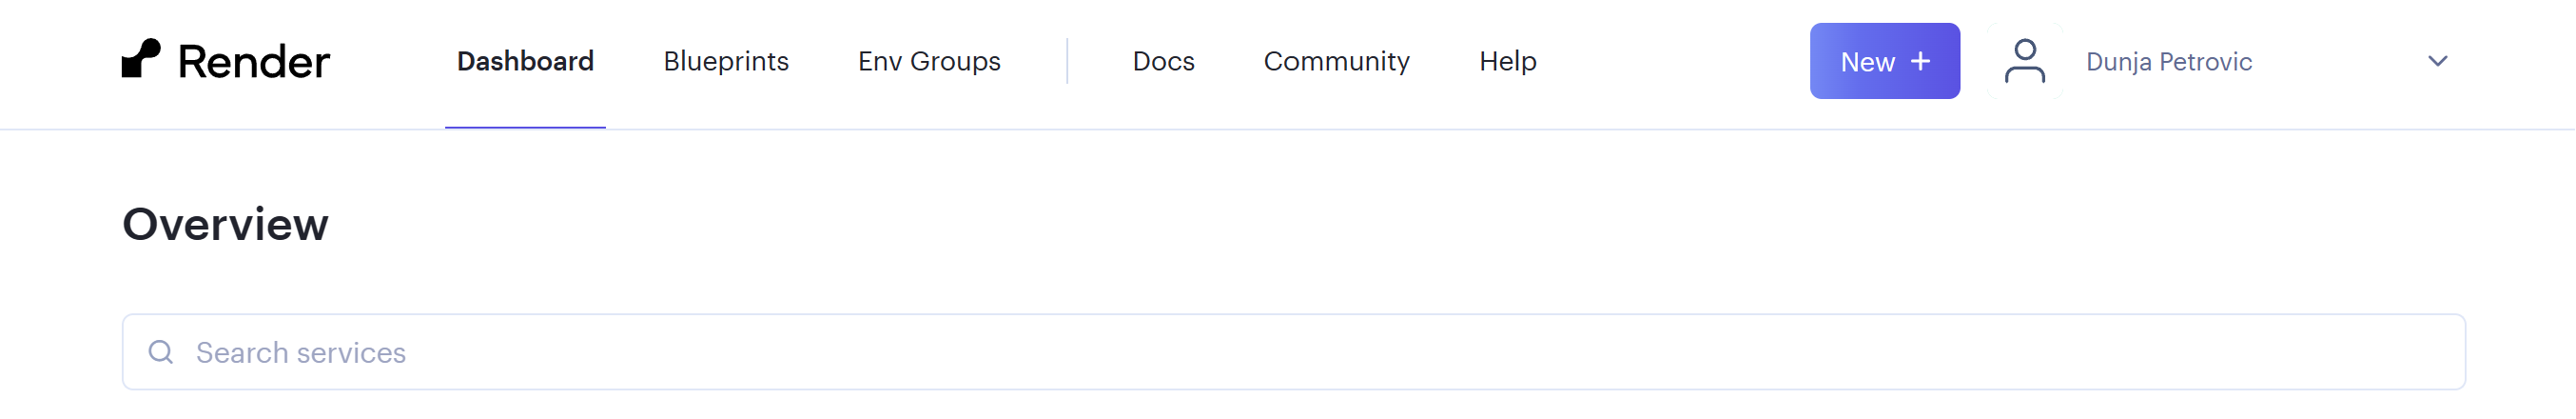
\includegraphics[scale=0.4]{slike/Render_NEW.PNG} %veličina slike u odnosu na originalnu datoteku i pozicija slike
			\centering
			\caption{Dodavanje nove komponente}
			\label{Dodavanje nove komponente}
		\end{figure}
		
		Zatim, u izborniku koji se prikaže, potrebno je odabrati opciju Web Service, kako je prikazano na slici ispod.
					\begin{figure}[H]
			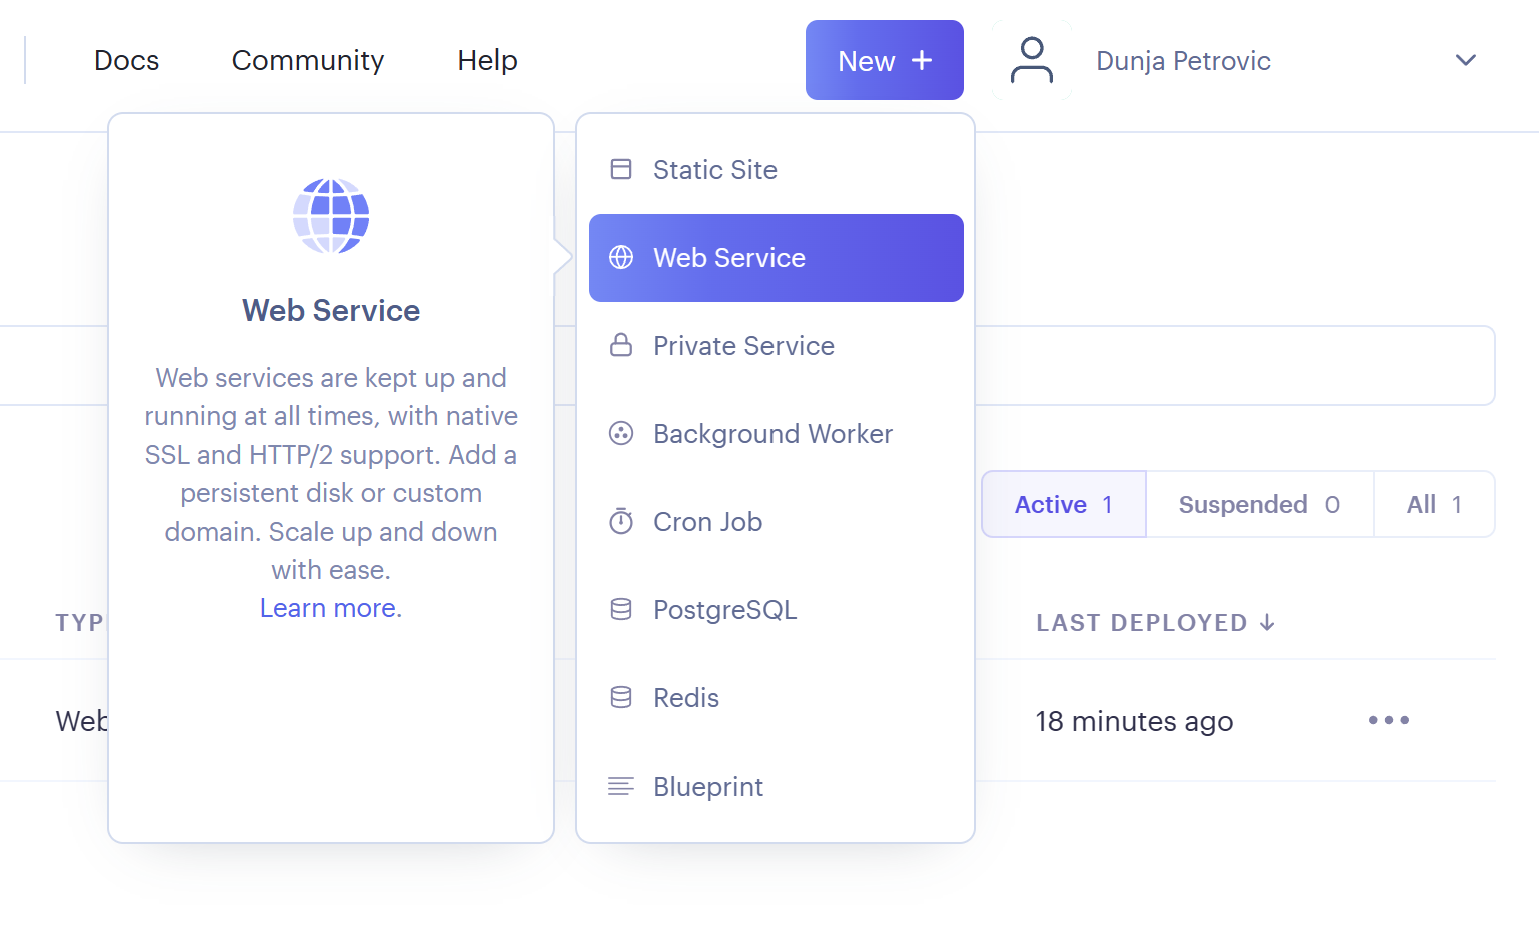
\includegraphics[scale=0.4]{slike/Render_WEB_SERVICE.PNG} %veličina slike u odnosu na originalnu datoteku i pozicija slike
			\centering
			\caption{Odabir opcije Web Service}
			\label{Odabir opcije Web Service}
		\end{figure}
		
		Kada nam se otvori stranica za dodavanje nove komponente tipa "Web Service", nudi nam se opcija odabira GitHub repozitorija iz koje želimo dodati komponentu, koju je potrebno i označiti, kako je prikazano na slici ispod.
		
			\begin{figure}[H]
			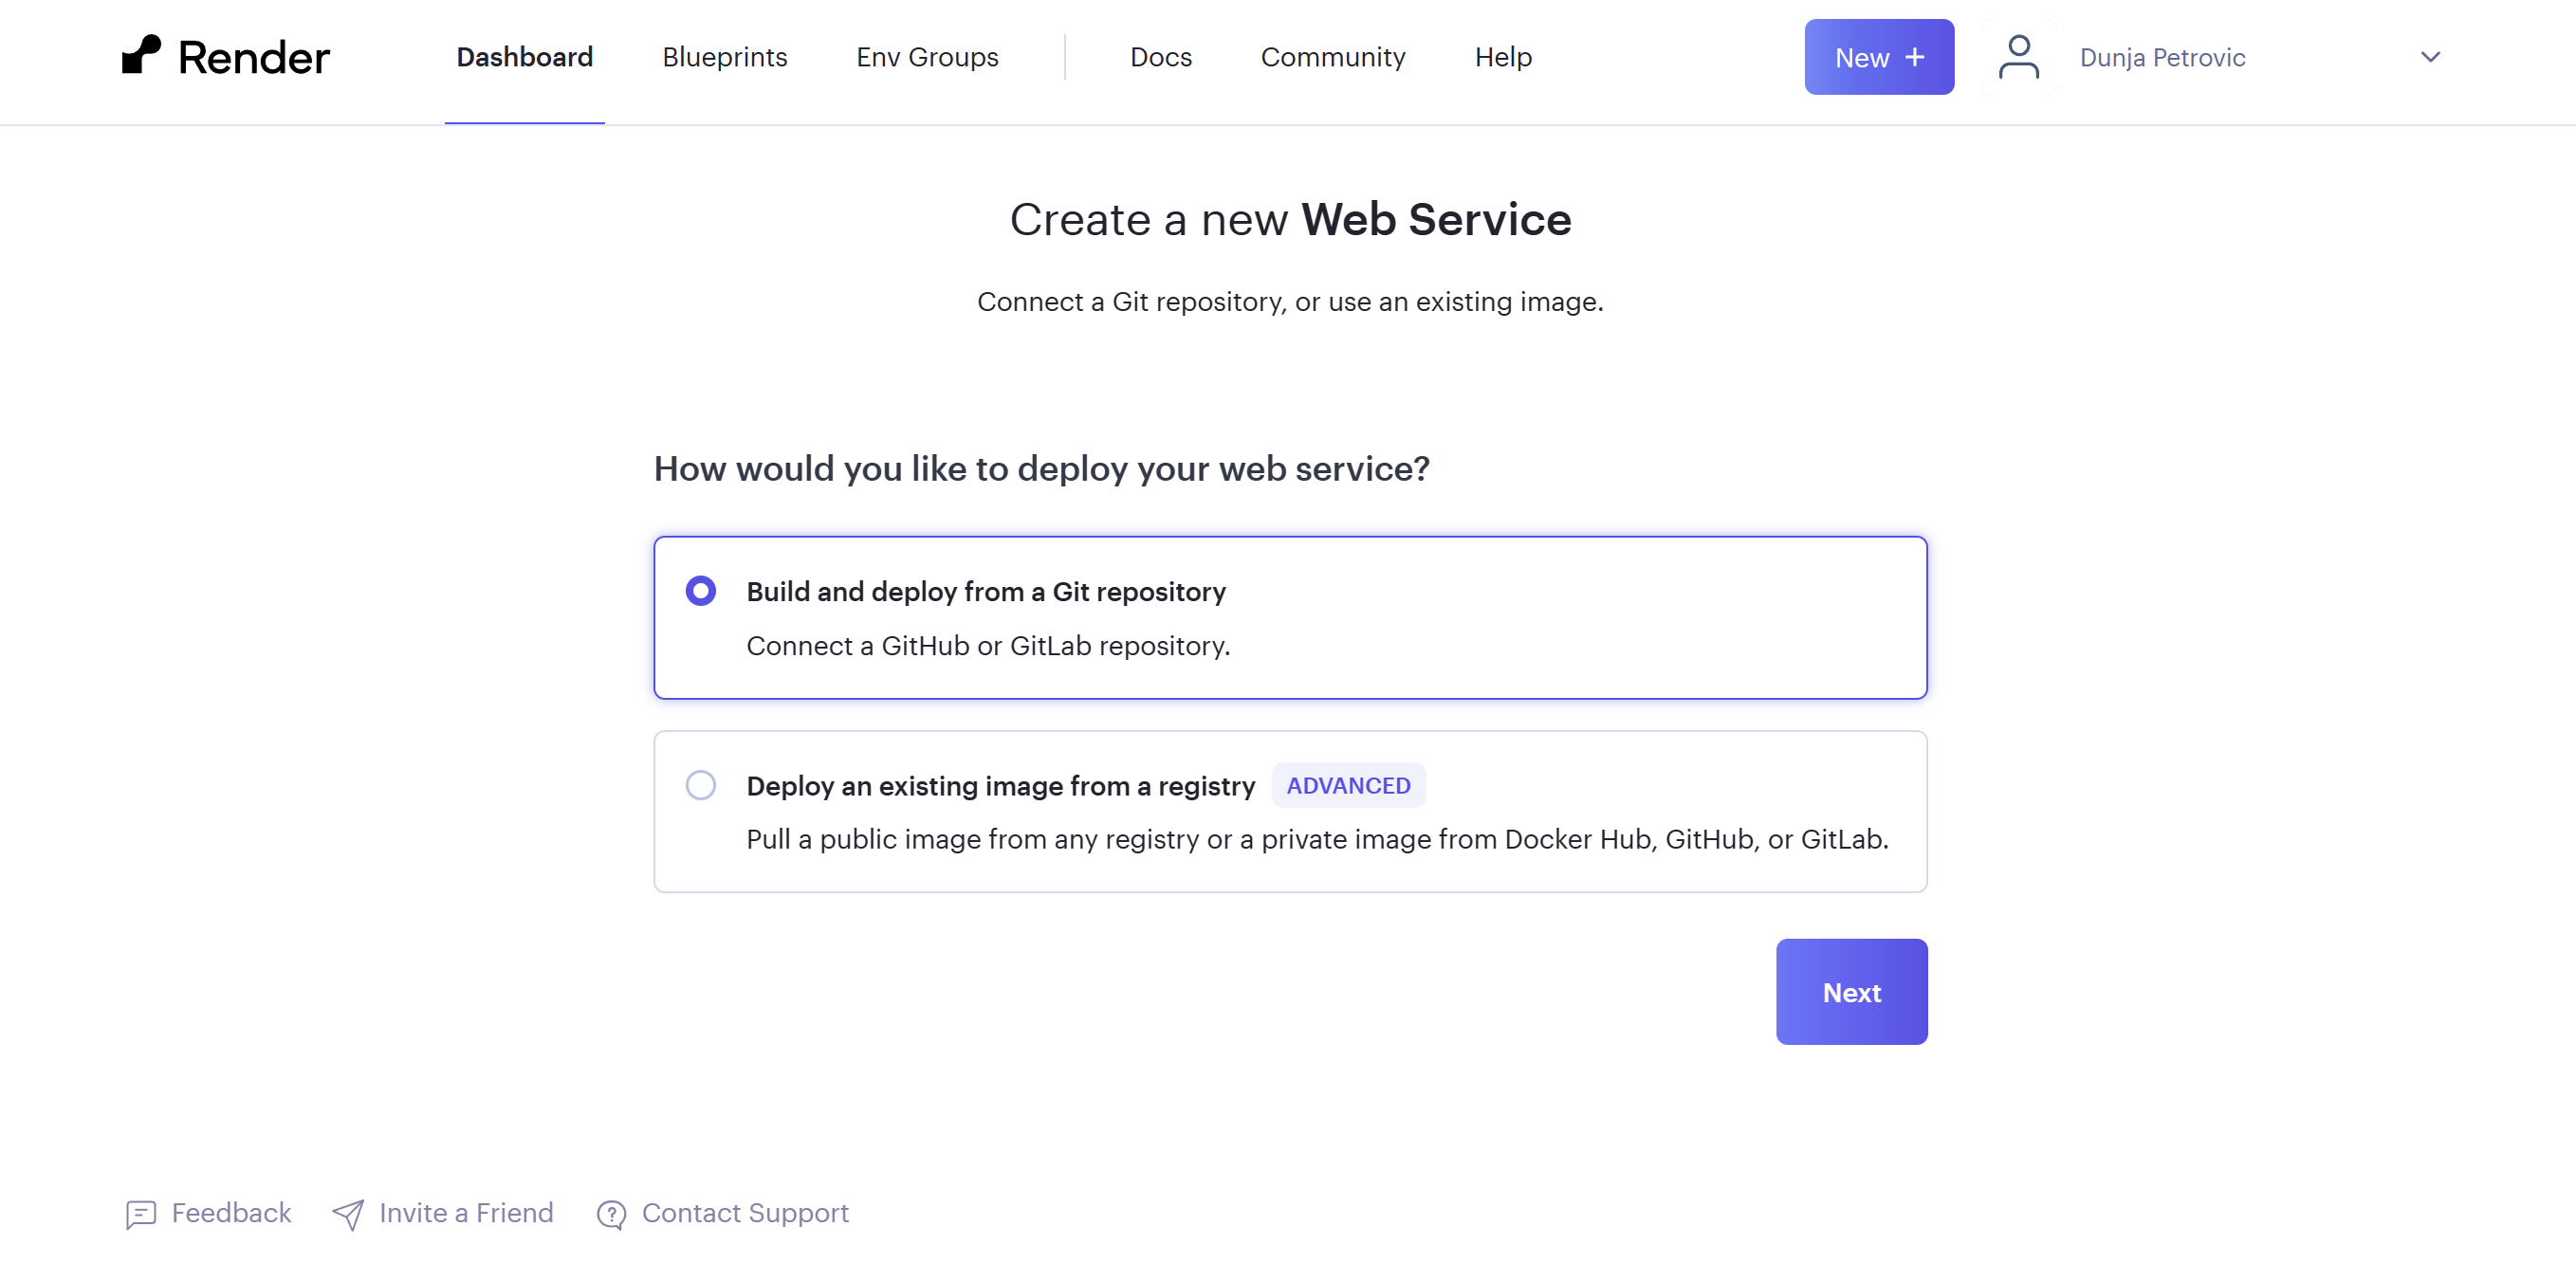
\includegraphics[scale=0.4]{slike/Render_ODABIR_OPCIJE.PNG} %veličina slike u odnosu na originalnu datoteku i pozicija slike
			\centering
			\caption{Odabir opcije dodavanja iz postojećeg GitHub repozitorija}
			\label{Odabir opcije dodavanja iz postojećeg GitHub repozitorija}
		\end{figure}
		
	    Nakon povezivanja Render računa s GitHub računom, slijedi odabir repozitorija, kako je prikazano na slici ispod. Mi smo odabrali repozitorij ljubo9/30bodova.
	    
	    	\begin{figure}[H]
			\includegraphics[scale=0.4]{slike/Render_ODABIR_REPOZITORIJA.PNG} %veličina slike u odnosu na originalnu datoteku i pozicija slike
			\centering
			\caption{Odabir repozitorija}
			\label{Odabir repozitorija}
		\end{figure}
		
		Odabir repozitorija slijedi podešavanje svih potrebnih opcija kako bi se Spring Boot poslužitelj ispravno pokrenuo. Na slici ispod prikazane su postavke koje je potrebno postaviti za ispravan rad poslužitelja.
		
		\begin{figure}[H]
			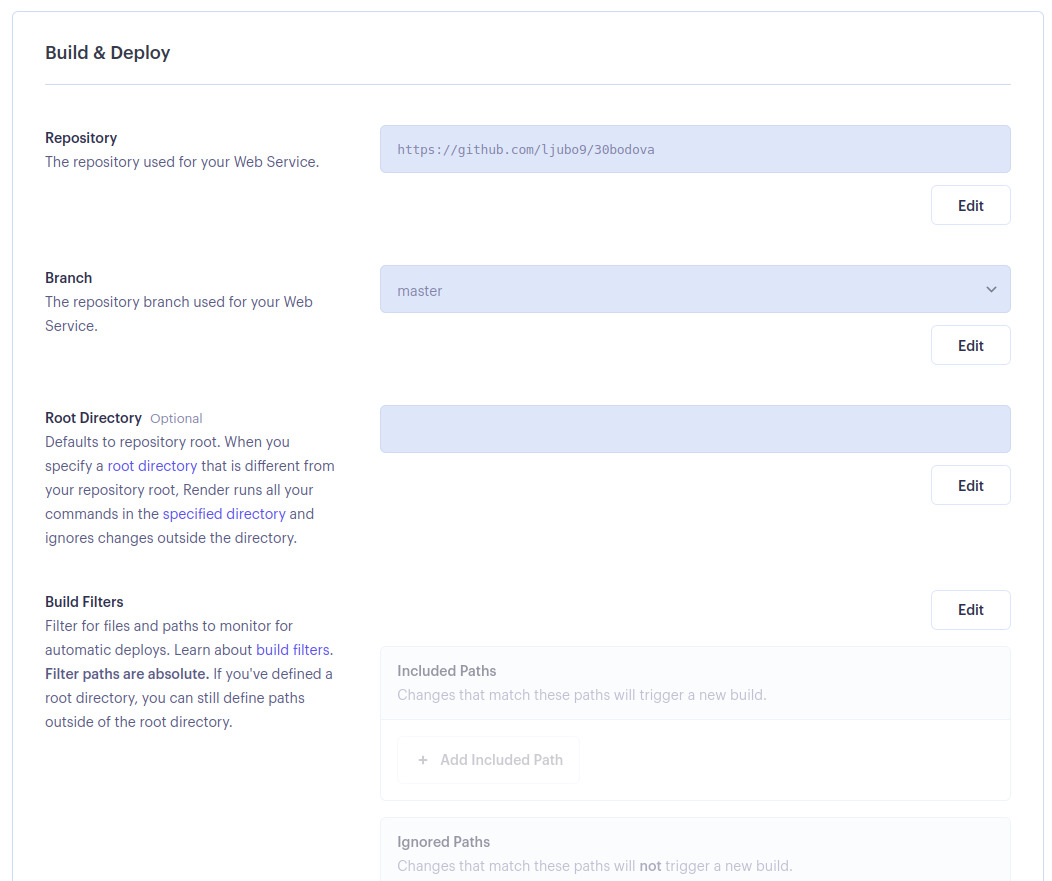
\includegraphics[scale=0.4]{slike/Render_BACKEND_1.JPG} %veličina slike u odnosu na originalnu datoteku i pozicija slike
			\centering
			\caption{Postavke za postavljanje Spring Boot poslužitelja, 1. dio}
			\label{Postavke za postavljanje Spring Boot poslužitelja, 1. dio}
		\end{figure}
		
		Na gornjoj je slici još jednom vidljiv odabrani repozitorij, odabrana grana (mi smo odabrali granu "master") i korijenski direktorij (nama to nije bilo važno pa smo ga ostavili praznog).
		
		Na slici ispod može se vidjeti drugi dio potrebnih postavki za postavljanje Spring Boot poslužitelja.
		
				\begin{figure}[H]
			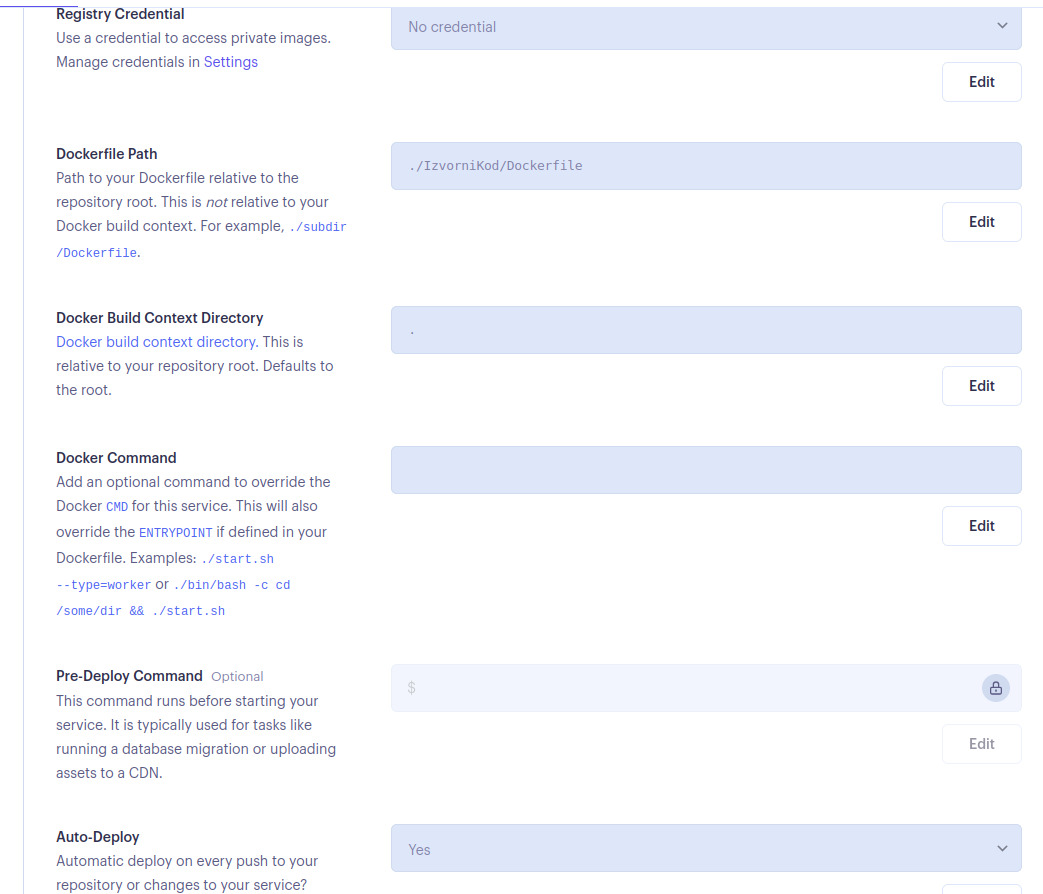
\includegraphics[scale=0.4]{slike/Render_BACKEND_2.JPG} %veličina slike u odnosu na originalnu datoteku i pozicija slike
			\centering
			\caption{Postavke za postavljanje Spring poslužitelja, 2. dio}
			\label{Postavke za postavljanje Spring poslužitelja, 2. dio}
		\end{figure}
		
		Ono što je bilo važno podesiti je bila lokacija Dockerfile-a, koju smo mi podesili na ./IzvorniKod/Dockerfile. Usto, označili smo i opciju "Auto-Deploy" s "Yes" , tako da se svaki put kada se neka nova izmjena napravi u kodu, Spring Boot poslužitelj se iznova "deploy-a". Time je deploy Spring Boot poslužitelja priveden kraju. \\
		
	\textbf{Postavljanje React web aplikacije} \\
	Kao i postavljanje Spring Boot poslužitelja, postavljanje React web aplikacije na Render je izrazito jednostavno. Svi koraci do podešavanja postavki za ispravan rad React web aplikacije jednaki su kao za postavljanje Spring Boot poslužitelja: dodavanje novog "web service-a", odabir opcije spajanja s GitHub repozitorijem, spajanje sa željenim GitHub računom te odabir GitHub repozitorija u kojem se nalazi projekt.
	
	Ono što se razlikuje je podešavanje ispravnih postavki za pokretanje React web aplikacije. Na slici ispod prikazane su potrebne postavke.
	
		\begin{figure}[H]
			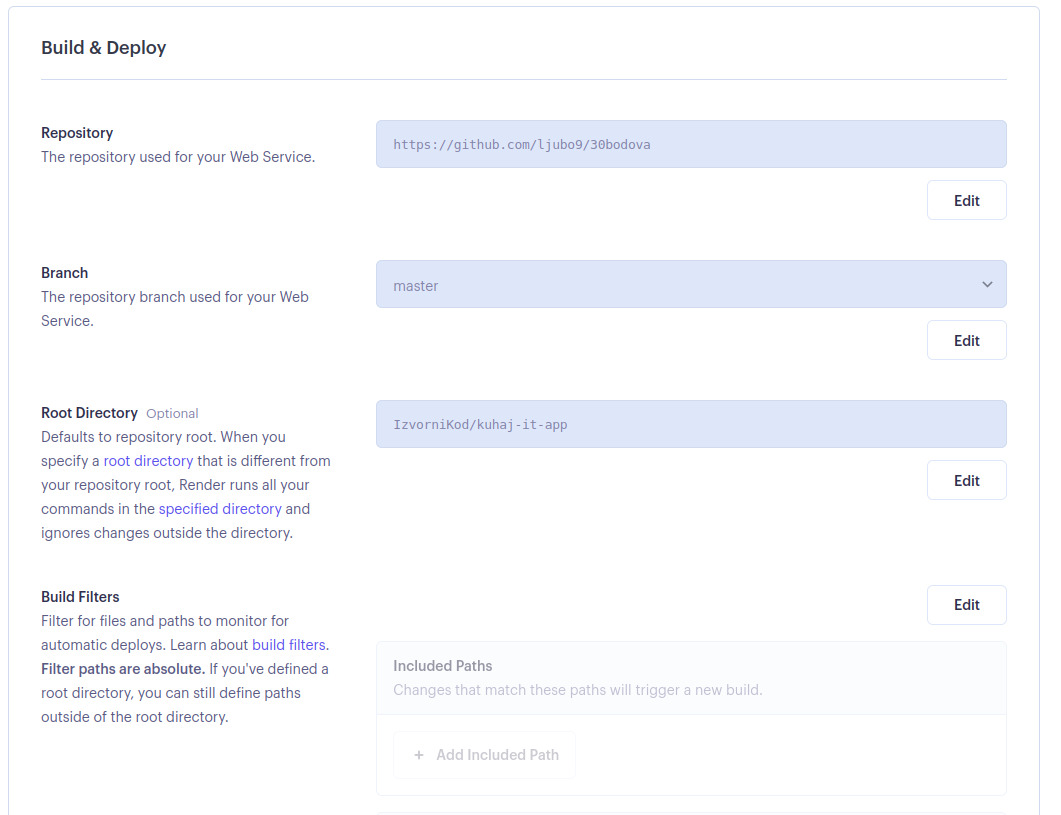
\includegraphics[scale=0.4]{slike/Render_FRONTEND_1.JPG} %veličina slike u odnosu na originalnu datoteku i pozicija slike
			\centering
			\caption{Postavke za postavljanje React web aplikacije, 1. dio}
			\label{Postavke za postavljanje React web aplikacije, 1. dio}
		\end{figure}
		
	Odabrani repozitorij isti je kao za postavljanje Spring Boot poslužitelja, kao i odabrana grana repozitorija.
	Za razliku od postavljanja Spring Boot poslužitelja, ovdje smo za korijenski direktorij odabrali direktorij IzvorniKod/kuhaj-it-app. Drugi dio potrebnih postavki prikazan je na slici ispod.
	
			\begin{figure}[H]
			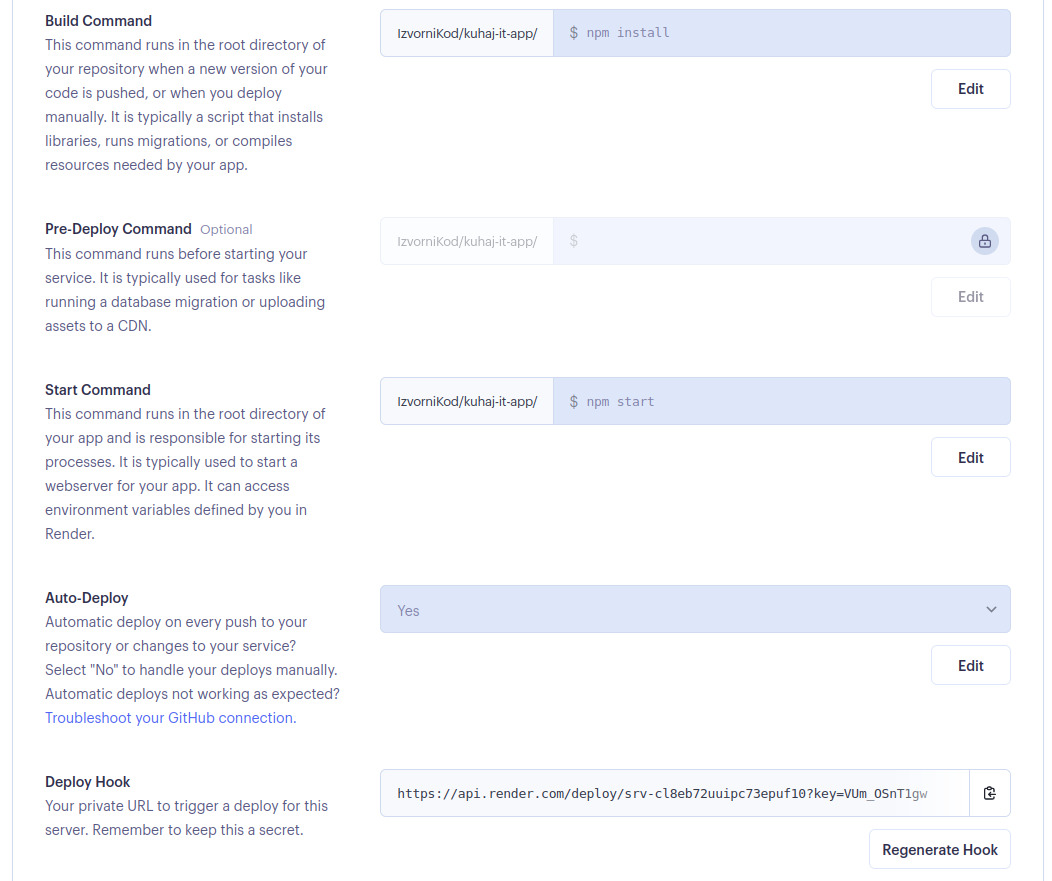
\includegraphics[scale=0.4]{slike/Render_FRONTEND_2.JPG} %veličina slike u odnosu na originalnu datoteku i pozicija slike
			\centering
			\caption{Postavke za postavljanje React web aplikacije, 2. dio}
			\label{Postavke za postavljanje React web aplikacije, 2. dio}
		\end{figure}
		
		Na gornjoj je slici vidljivo da smo za "naredbu izgradnje", naredbu koja će instalirati sve biblioteke, pokrenuti migracije i kompajlirati sve potrebno za ispravan rad naše React web aplikacije, odabrali naredbu "npm install".
		Ono što je još trebalo podesiti je naredba pokretanja, koju smo podesili na "npm start".
		Isto kao i kod podešavanja Spring Boot poslužitelja, odabrali smo opciju Auto-Deploy. \\
		
				\textbf{Postavljanje baze podataka} \\
				Iako nešto drugačije od "deploy-anja" Spring Boot poslužitelja i React web aplikacije, postavljanje PostgreSQL baze podataka na platformu Render također je izrazito jednostavno. \\
				Za početak, potrebno je na početnoj stranici stisnuti gumb New, a zatim odabrati opciju PostgreSQL, kako je prikazano na slici ispod.
				
				\begin{figure}[H]
			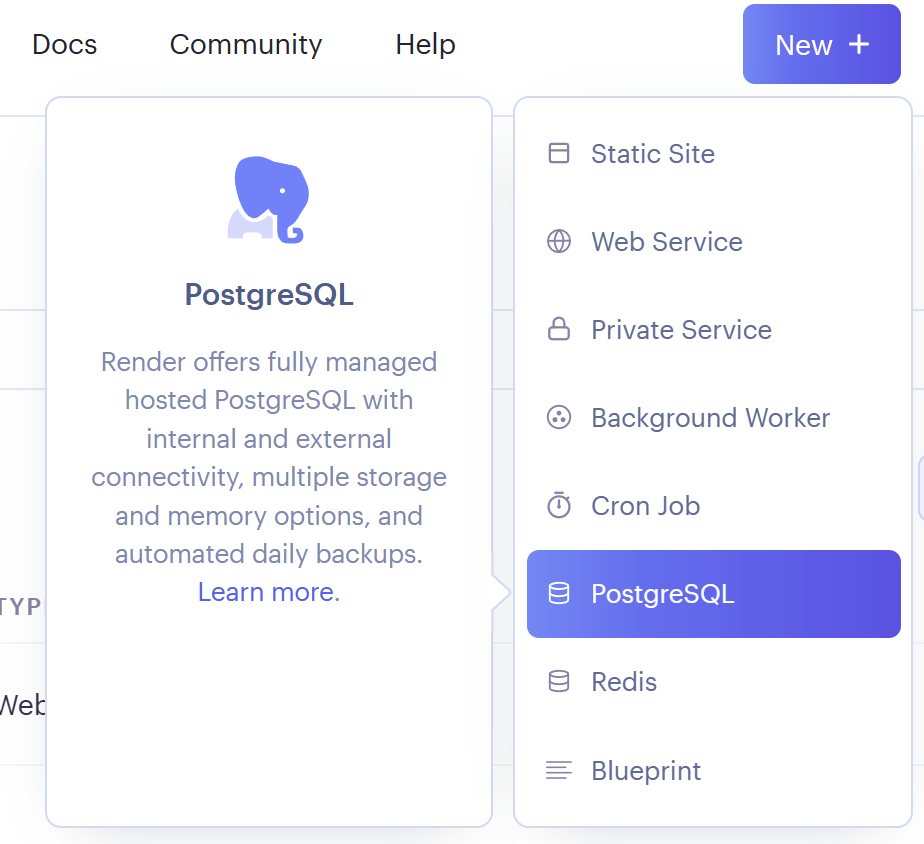
\includegraphics[scale=0.4]{slike/Render_PostgreSQL.PNG} %veličina slike u odnosu na originalnu datoteku i pozicija slike
			\centering
			\caption{Dodavanje nove PostgreSQL baze podataka}
			\label{Dodavanje nove PostgreSQL baze podataka}
		\end{figure}
		
		Odabirom opcije PostgreSQL, otvara se novi prozor na kojem je moguće unijeti razne podatke o bazi podataka: ime, korisnika, verziju PostgreSQL-a itd. Podatke koje smo mi unijeli prikazani su na slikama ispod.
		
			\begin{figure}[H]
			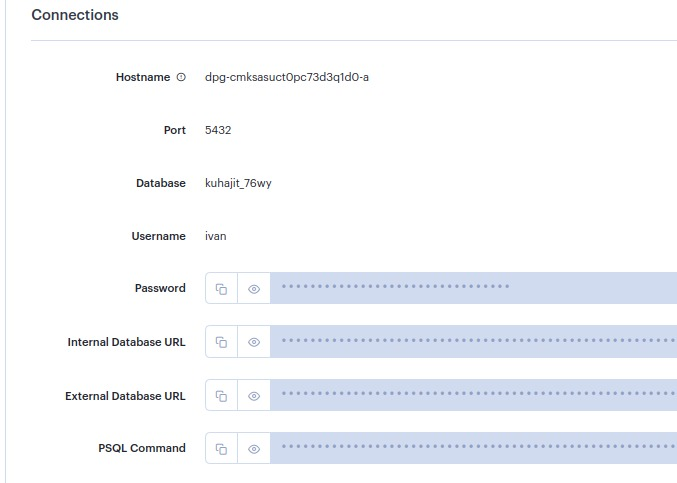
\includegraphics[scale=0.4]{slike/Render_DATABASE_1.JPG} %veličina slike u odnosu na originalnu datoteku i pozicija slike
			\centering
			\caption{Postavke baze podataka na Render-u, 1. dio}
			\label{Postavke baze podataka na Render-u, 1. dio}
		\end{figure}
		
		\begin{figure}[H]
			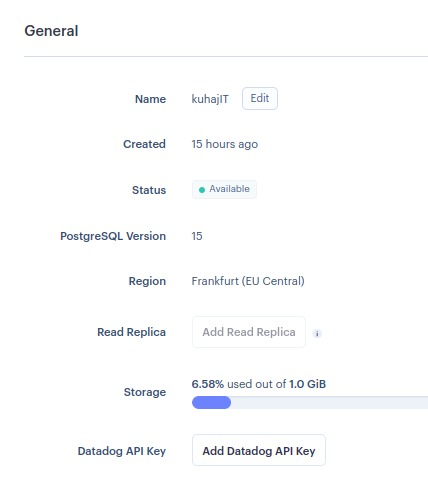
\includegraphics[scale=0.4]{slike/Render_DATABASE_2.JPG} %veličina slike u odnosu na originalnu datoteku i pozicija slike
			\centering
			\caption{Postavke baze podataka na Render-u, 2. dio}
			\label{Postavke baze podataka na Render-u, 2. dio}
		\end{figure}
		
		Postavka "Password" šifra je usera koja služi za spajanje na bazu i vidljiva je u datoteci application.properties, dok su polja Internal Database URL, External Database URL i PSQL Command generirana od strane platforme Render.
		
		Stvorena baza podataka je prazna, a mi ju moramo napuniti podacima. Skripta za izravno punjenje baze podataka (inicijaliziranje svih tablica i veza između njih te punjenje nekim testnim podacima) nalazi se u datoteci Script.sql, a mi smo ju pokretali izravno iz razvojnog okruženja Eclipse IDE.
		
				
	
		
	
	
	
		
		
		
		
		
		
		
		
		 
		
		
	    
	    
		
		
		
		
		
		
		
			
			\eject 
	\chapter{Zaključak i budući rad}
		
		17 tjedana nakon prvog okupljanja projektne grupe, naš je zadatak priveden kraju. Implementirali smo web aplikaciju za sve one koji su zainteresirani za kvalitetnu prehranu. Ostvarena je registracija i prijava korisnika u tri kategorije: "običnih" klijenata, kulinarskih entuzijasta i nutricionista. 
		"Obični" klijent na našoj KuhajIT aplikaciji ima, uz mogućnost pretraživanja kulinarskih entuzijasta i pregleda njihovih recepata, što može i neregistrirani korisnik, mogućnost skeniranja ili ručnog unosa sastojaka koje ima doma i koje želi upotrijebiti za pripravu recepta, na temelju kojih mu aplikacija generira najprikladnije recepte. Također, klijent ima mogućnost i označiti konzumirane recepte, zapratiti željene kulinarske entuzijaste te putem aplikacije pratiti dijetu koju kreira nutricionist.
		Kulinarski entuzijast ima sve mogućnosti "običnog" klijenta, no tu je i mogućnost stvaranja kuharica i recepata, koje objavljuje na aplikaciji. 
		Nutricionist također ima sve mogućnosti "običnog" klijenta, uz opciju unošenja nutritivnih podataka o sastojcima te kreiranje dijeta sa željenim ograničenjima.
		Izrada čitave ove funkcionalnosti bila je podijeljena u dva dijela: tzv. "prvi" i "drugi" ciklus.
		Prvi ciklus nije bio toliko zahtjevan što se same implementacije tiče, no ima ogromnu težinu zbog važnosti svih odluka donesenih upravo tijekom njega, od okupljanja projektne grupe, preko konceptualnog osmišljavanja same implementacije, pa sve do postavljanja čvrstih temelja na koje se naprednija implementacija nadograđivala. Značajan dio rada u prvom ciklusu bilo je opširno dokumentiranje čitavog projektnog zadatka: opis projektnog zadatka, specifikacija programske potpore (koja je uključivala obrasce uporabe te pripadajuće dijagrame obrazaca uporabe te sekvencijske dijagrame) i opis arhitekture (dizajn baze podataka te dijagrami razreda). 
		Drugi ciklus bio je prilično implementacijski zahtjevniji. Većina konkretne implementacije web aplikacije ostvarena je upravo u drugom ciklusu, uz manje, ali ne manje važne dopune dokumentaciji (dijagrami stanja, aktivnosti, komponenti, razmještaja itd.). U ovom se ciklusu većina članova tima susrela s prvim ozbiljnijim radom u njima nepoznatim tehnologijama, što je iziskivalo određeno vrijeme upoznavanja, istraživanja i prilagodbe novome. Ne treba zanemariti niti vrijeme uloženo u pažljivo testiranje rada aplikacije pomoću unit i selenium testova, a koje je opisano u jednom od gornjih poglavlja, kao niti tzv. "deployment" naše web aplikacije.
		Tijekom implementacije, dogovori između članova tima tekli su putem WhatsApp grupe, što nam se pokazalo vrlo korisnim jer su na taj način svi članovi tima, čak i oni koji u dotičnom dijelu implementacije nisu direktno sudjelovali, bili upućeni u trenutno stanje.
		Prostora za napredak uvijek ima, neke od ideja koje smo imali su stvaranje personaliziranih dijeta na zahtjev klijenata, stvaranje mobilne verzije aplikacije KuhajIT, unapređenje sučelja i dr.
		Uz sve gore navedeno, upoznavanje s novim tehnologijama, učenje pravilnog dokumentiranja, "deployanja" i slično, najvažnija tekovina ovog projekta svim je članovima upravo rad u timu. Iako nije u svim trenucima bilo jednostavno, svi smo naučili vrijedne lekcije o timskom radu, međusobnoj potpori, organizaciji vremena i vrijednostima koje ćemo tražiti i u nekim budućim projektnim grupama.
		S obzirom na to da nam je svima to prvo iskustvo ovakvoga tipa, a i na ostale obaveze koje svi imamo na fakultetu, ponosni smo na obavljeno.
				\eject 
	\chapter*{Popis literature}
		\addcontentsline{toc}{chapter}{Popis literature}
	 	
 		\textbf{\textit{Kontinuirano osvježavanje}}
	
		\textit{Popisati sve reference i literaturu koja je pomogla pri ostvarivanju projekta.}
		
		
		\begin{enumerate}
			
			
			\item  Programsko inženjerstvo, FER ZEMRIS, \url{http://www.fer.hr/predmet/proinz}
			
			\item  I. Sommerville, "Software engineering", 8th ed, Addison Wesley, 2007.
			
			\item  T.C.Lethbridge, R.Langaniere, "Object-Oriented Software Engineering", 2nd ed. McGraw-Hill, 2005.
			
			\item  I. Marsic, Software engineering book``, Department of Electrical and Computer Engineering, Rutgers University, \url{http://www.ece.rutgers.edu/~marsic/books/SE}
			
			\item  The Unified Modeling Language, \url{https://www.uml-diagrams.org/}
			
			\item  Astah Community, \url{http://astah.net/editions/uml-new}
		\end{enumerate}
		
		 
	\chapter*{Dodatak: Prikaz aktivnosti grupe}
		\addcontentsline{toc}{chapter}{Dodatak: Prikaz aktivnosti grupe}
		
		\section*{Dnevnik sastajanja}

		\begin{packed_enum}
			\item  sastanak
			
			\item[] \begin{packed_item}
				\item Datum: u ovom formatu: 16.listopada 2023.
				\item Prisustvovali: H.Ivančić, D.Ljubić, I.Pavlović, M.Perković, D.Petrović, K.Raštegorac, F.Širić
				\item Teme sastanka:
				\begin{packed_item}
					\item  upoznavanje s temom
				\end{packed_item}
			\end{packed_item}
			
			\item  sastanak
			\item[] \begin{packed_item}
				\item Datum: u ovom formatu: 25.listopada 2023.
				\item Prisustvovali: H.Ivančić, I.Pavlović, M.Perković, D.Petrović, K.Raštegorac, F.Širić
				\item Teme sastanka:
				\begin{packed_item}
					\item  raspodjela posla
					\item  početak rada
				\end{packed_item}
			\end{packed_item}
			
			\item  sastanak
			\item[] \begin{packed_item}
				\item Datum: 2.studenoga 2023.
				\item Prisustvovali: H.Ivančić, D.Ljubić, I.Pavlović, M.Perković, D.Petrović, K.Raštegorac, F.Širić
				\item Teme sastanka:
				\begin{packed_item}
					\item  provjera dotad završene dokumentacije
					\item detaljnija raspodjela posla
				\end{packed_item}
			\end{packed_item}
			
			\item  sastanak
			\item[] \begin{packed_item}
				\item Datum: 9.studenoga 2023.
				\item Prisustvovali: H.Ivančić, D.Ljubić, I.Pavlović, M.Perković, D.Petrović, K.Raštegorac, F.Širić
				\item Teme sastanka:
				\begin{packed_item}
					\item  testiranje dotad dovršene implementacije
					\item  provjera dotad završene dokumentacije
				\end{packed_item}
			\end{packed_item}
			
			\item  sastanak
			\item[] \begin{packed_item}
				\item Datum: 17.studenoga 2023.
				\item Prisustvovali: H.Ivančić, D.Ljubić, I.Pavlović, M.Perković, D.Petrović, K.Raštegorac, F.Širić
				\item Teme sastanka:
				\begin{packed_item}
					\item  posljednja provjera ispravnosti dokumentacije
					\item  posljednja provjera implementacije funkcionalnosti
				\end{packed_item}
			\end{packed_item}
			
			\item  sastanak
			\item[] \begin{packed_item}
				\item Datum: 11.prosinca 2023.
				\item Prisustvovali: H.Ivančić, D.Ljubić, I.Pavlović, M.Perković, D.Petrović, K.Raštegorac, F.Širić
				\item Teme sastanka:
				\begin{packed_item}
					\item  dogovor o daljnjem tijeku rada
					\item zadavanje ciljeva implementacije za 2. ciklus
				\end{packed_item}
			\end{packed_item}
			
			\item  sastanak
						\item[] \begin{packed_item}
				\item Datum: 18.prosinca 2023.
				\item Prisustvovali: H.Ivančić, D.Ljubić, I.Pavlović, M.Perković, D.Petrović, K.Raštegorac, F.Širić
				\item Teme sastanka:
				\begin{packed_item}
					\item statusni sastanak
					\item plan daljnjeg rada
				\end{packed_item}
			\end{packed_item}
			
			\item  sastanak
			\begin{packed_item}
				\item Datum: 29.prosinca 2023.
				\item Prisustvovali: H.Ivančić, D.Ljubić, M.Perković, K.Raštegorac, F.Širić
				\item Teme sastanka:
				\begin{packed_item}
					\item dogovor o dijelovima frontend aplikacije
				\end{packed_item}
			\end{packed_item}
			
						\item  sastanak
						\begin{packed_item}
				\item Datum: 5.siječnja 2024.
				\item Prisustvovali: H.Ivančić, D.Ljubić, I.Pavlović, M.Perković, D.Petrović, K.Raštegorac, F.Širić
				\item Teme sastanka:
				\begin{packed_item}
					\item statusni sastanak
					\item konzultacije o izradi preostalog dijela dokumentacije
				\end{packed_item}
			\end{packed_item}
			
					\item sastanak				\begin{packed_item}
				\item Datum: 12.siječnja 2024.
				\item Prisustvovali: H.Ivančić, D.Ljubić, I.Pavlović, M.Perković, D.Petrović, K.Raštegorac, F.Širić
				\item Teme sastanka:
				\begin{packed_item}
					\item briefing dotad implementiranog
					\item posljednje izmjene baze podataka
				\end{packed_item}
			\end{packed_item}
			
						\item  sastanak
		\begin{packed_item}
				\item Datum: 13.siječnja 2024.
				\item Prisustvovali: H.Ivančić, D.Ljubić, I.Pavlović, M.Perković, D.Petrović, K.Raštegorac, F.Širić
				\item Teme sastanka:
				\begin{packed_item}
					\item briefing dotad implementiranog
					\item posljednje izmjene baze podataka
				\end{packed_item}
			\end{packed_item}
			
						\item  sastanak
					\begin{packed_item}
				\item Datum: 16.siječnja 2024.
				\item Prisustvovali: H.Ivančić, D.Ljubić, I.Pavlović, M.Perković, D.Petrović, K.Raštegorac, F.Širić
				\item Teme sastanka:
				\begin{packed_item}
					\item briefing dotad implementiranog
				\end{packed_item}
			\end{packed_item}
			
						\item  sastanak					\begin{packed_item}
				\item Datum: 19.siječnja 2024.
				\item Prisustvovali: H.Ivančić, D.Ljubić, I.Pavlović, M.Perković, D.Petrović, K.Raštegorac, F.Širić
				\item Teme sastanka:
				\begin{packed_item}
					\item posljednje izmjene dokumentacije
					\item posljednja provjera inmplementacije
				\end{packed_item}
			\end{packed_item}
			
			
			
			%
			
		\end{packed_enum}
		
		\eject
		\section*{Tablica aktivnosti}
		
			\textbf{\textit{Kontinuirano osvježavanje}}\\
			
			 \textit{Napomena: Doprinose u aktivnostima treba navesti u satima po članovima grupe po aktivnosti.}

			\begin{longtblr}[
					label=none,
				]{
					vlines,hlines,
					width = \textwidth,
					colspec={X[7, l]X[1, c]X[1, c]X[1, c]X[1, c]X[1, c]X[1, c]X[1, c]}, 
					vline{1} = {1}{text=\clap{}},
					hline{1} = {1}{text=\clap{}},
					rowhead = 1,
				} 
			
				\SetCell[c=1]{c}{} & \SetCell[c=1]{c}{\rotatebox{90}{\textbf{Hana Ivančić}}} & \SetCell[c=1]{c}{\rotatebox{90}{\textbf{David Ljubić}}} &	\SetCell[c=1]{c}{\rotatebox{90}{\textbf{Ivan Pavlović}}} & \SetCell[c=1]{c}{\rotatebox{90}{\textbf{Marija Perković}}} &	\SetCell[c=1]{c}{\rotatebox{90}{\textbf{Dunja Petrović}}} & \SetCell[c=1]{c}{\rotatebox{90}{\textbf{Karlo Raštegorac}}} &	\SetCell[c=1]{c}{\rotatebox{90}{\textbf{Fran Širić}}} \\  
				Upravljanje projektom 		& 10 &  1&  &  &  2&  & \\ 
				Opis projektnog zadatka 	&  &  &  &  &  4&  & \\ 
				
				Funkcionalni zahtjevi       & 3 &  &  &  & 7 &  &  \\ 
				Opis pojedinih obrazaca 	&  1&  &  &  & 5 &  &  \\ 
				Dijagram obrazaca 			& 6 &  &  &  & 2 &  &  \\ 
				Sekvencijski dijagrami 		&  5&  &  &  & 2 &  &  \\ 
				Opis ostalih zahtjeva 		&  &  &  &  & 1 &  &  \\ 

				Arhitektura i dizajn sustava	 &  &  &  &  &8  &  &  \\ 
				Baza podataka				&  &  &  &  &  5&  &   \\ 
				Dijagram razreda 			& 6 &  &  &  &  2&  &   \\ 
				Dijagram stanja				&  &  &  &  &  &  &  \\ 
				Dijagram aktivnosti 		&  &  &  &  &  &  &  \\ 
				Dijagram komponenti			&  &  &  &  &  &  &  \\ 
				Korištene tehnologije i alati 		& 2 & 2  & 2 & 2 & 2 & 2 & 5 \\ 
				Ispitivanje programskog rješenja 	&  & 2 &  & 5 &  &2  & 10 \\ 
				Dijagram razmještaja			&  &  &  &  &  &  &  \\ 
				Upute za puštanje u pogon 		&  &  &  &  &  &  &  \\  
				Dnevnik sastajanja 			&  &  &  &  & 1 &  &  \\ 
				Zaključak i budući rad 		&  &  &  &  &  &  &  \\  
				Popis literature 			&  &  &  &  & 1 &  &  \\  
				&  &  &  &  &  &  &  \\ \hline 
				\textit{Dodatne stavke kako ste podijelili izradu aplikacije} 			&  &  &  &  &  &  &  \\ 
				\textit{npr. izrada početne stranice} 				&  &  10 &  & 12 &  & 10 &  \\  
				\textit{izrada baze podataka} 		 			&  &  & 16 &  &  &  & 5\\  
				\textit{spajanje s bazom podataka} 							&  &  & 2 &  &  &  & 2 \\ 
				\textit{back end} 							&  &  &  &  &  &  & 30 \\ 
				\textit{deploy} 							& 10  & 1 & 1 & 1 & 1 & 1 & 1 \\  
				 							&  &  &  &  &  &  &\\ 
			\end{longtblr}

\end{document} %naredbe i tekst nakon ove naredbe ne ulaze u izgrađen dokument 


